\documentclass[10pt,]{book}
\usepackage{lmodern}
\usepackage{setspace}
\setstretch{1.1}
\usepackage{amssymb,amsmath}
\usepackage{ifxetex,ifluatex}
\usepackage{fixltx2e} % provides \textsubscript
\ifnum 0\ifxetex 1\fi\ifluatex 1\fi=0 % if pdftex
  \usepackage[T1]{fontenc}
  \usepackage[utf8]{inputenc}
\else % if luatex or xelatex
  \ifxetex
    \usepackage{mathspec}
  \else
    \usepackage{fontspec}
  \fi
  \defaultfontfeatures{Ligatures=TeX,Scale=MatchLowercase}
\fi
% use upquote if available, for straight quotes in verbatim environments
\IfFileExists{upquote.sty}{\usepackage{upquote}}{}
% use microtype if available
\IfFileExists{microtype.sty}{%
\usepackage{microtype}
\UseMicrotypeSet[protrusion]{basicmath} % disable protrusion for tt fonts
}{}
\usepackage[margin=1in]{geometry}
\usepackage{hyperref}
\hypersetup{unicode=true,
            pdftitle={Causal Inference Book: Exercises -- R code},
            pdfauthor={Book by M. A. Hernán and J. M. Robins, R code by Joy Shi and Sean McGrath, R Markdown code by Tom Palmer},
            pdfborder={0 0 0},
            breaklinks=true}
\urlstyle{same}  % don't use monospace font for urls
\usepackage{natbib}
\bibliographystyle{plainnat}
\usepackage{color}
\usepackage{fancyvrb}
\newcommand{\VerbBar}{|}
\newcommand{\VERB}{\Verb[commandchars=\\\{\}]}
\DefineVerbatimEnvironment{Highlighting}{Verbatim}{commandchars=\\\{\}}
% Add ',fontsize=\small' for more characters per line
\usepackage{framed}
\definecolor{shadecolor}{RGB}{248,248,248}
\newenvironment{Shaded}{\begin{snugshade}}{\end{snugshade}}
\newcommand{\AlertTok}[1]{\textcolor[rgb]{0.94,0.16,0.16}{#1}}
\newcommand{\AnnotationTok}[1]{\textcolor[rgb]{0.56,0.35,0.01}{\textbf{\textit{#1}}}}
\newcommand{\AttributeTok}[1]{\textcolor[rgb]{0.77,0.63,0.00}{#1}}
\newcommand{\BaseNTok}[1]{\textcolor[rgb]{0.00,0.00,0.81}{#1}}
\newcommand{\BuiltInTok}[1]{#1}
\newcommand{\CharTok}[1]{\textcolor[rgb]{0.31,0.60,0.02}{#1}}
\newcommand{\CommentTok}[1]{\textcolor[rgb]{0.56,0.35,0.01}{\textit{#1}}}
\newcommand{\CommentVarTok}[1]{\textcolor[rgb]{0.56,0.35,0.01}{\textbf{\textit{#1}}}}
\newcommand{\ConstantTok}[1]{\textcolor[rgb]{0.00,0.00,0.00}{#1}}
\newcommand{\ControlFlowTok}[1]{\textcolor[rgb]{0.13,0.29,0.53}{\textbf{#1}}}
\newcommand{\DataTypeTok}[1]{\textcolor[rgb]{0.13,0.29,0.53}{#1}}
\newcommand{\DecValTok}[1]{\textcolor[rgb]{0.00,0.00,0.81}{#1}}
\newcommand{\DocumentationTok}[1]{\textcolor[rgb]{0.56,0.35,0.01}{\textbf{\textit{#1}}}}
\newcommand{\ErrorTok}[1]{\textcolor[rgb]{0.64,0.00,0.00}{\textbf{#1}}}
\newcommand{\ExtensionTok}[1]{#1}
\newcommand{\FloatTok}[1]{\textcolor[rgb]{0.00,0.00,0.81}{#1}}
\newcommand{\FunctionTok}[1]{\textcolor[rgb]{0.00,0.00,0.00}{#1}}
\newcommand{\ImportTok}[1]{#1}
\newcommand{\InformationTok}[1]{\textcolor[rgb]{0.56,0.35,0.01}{\textbf{\textit{#1}}}}
\newcommand{\KeywordTok}[1]{\textcolor[rgb]{0.13,0.29,0.53}{\textbf{#1}}}
\newcommand{\NormalTok}[1]{#1}
\newcommand{\OperatorTok}[1]{\textcolor[rgb]{0.81,0.36,0.00}{\textbf{#1}}}
\newcommand{\OtherTok}[1]{\textcolor[rgb]{0.56,0.35,0.01}{#1}}
\newcommand{\PreprocessorTok}[1]{\textcolor[rgb]{0.56,0.35,0.01}{\textit{#1}}}
\newcommand{\RegionMarkerTok}[1]{#1}
\newcommand{\SpecialCharTok}[1]{\textcolor[rgb]{0.00,0.00,0.00}{#1}}
\newcommand{\SpecialStringTok}[1]{\textcolor[rgb]{0.31,0.60,0.02}{#1}}
\newcommand{\StringTok}[1]{\textcolor[rgb]{0.31,0.60,0.02}{#1}}
\newcommand{\VariableTok}[1]{\textcolor[rgb]{0.00,0.00,0.00}{#1}}
\newcommand{\VerbatimStringTok}[1]{\textcolor[rgb]{0.31,0.60,0.02}{#1}}
\newcommand{\WarningTok}[1]{\textcolor[rgb]{0.56,0.35,0.01}{\textbf{\textit{#1}}}}
\usepackage{longtable,booktabs}
\usepackage{graphicx,grffile}
\makeatletter
\def\maxwidth{\ifdim\Gin@nat@width>\linewidth\linewidth\else\Gin@nat@width\fi}
\def\maxheight{\ifdim\Gin@nat@height>\textheight\textheight\else\Gin@nat@height\fi}
\makeatother
% Scale images if necessary, so that they will not overflow the page
% margins by default, and it is still possible to overwrite the defaults
% using explicit options in \includegraphics[width, height, ...]{}
\setkeys{Gin}{width=\maxwidth,height=\maxheight,keepaspectratio}
\IfFileExists{parskip.sty}{%
\usepackage{parskip}
}{% else
\setlength{\parindent}{0pt}
\setlength{\parskip}{6pt plus 2pt minus 1pt}
}
\setlength{\emergencystretch}{3em}  % prevent overfull lines
\providecommand{\tightlist}{%
  \setlength{\itemsep}{0pt}\setlength{\parskip}{0pt}}
\setcounter{secnumdepth}{0}
% Redefines (sub)paragraphs to behave more like sections
\ifx\paragraph\undefined\else
\let\oldparagraph\paragraph
\renewcommand{\paragraph}[1]{\oldparagraph{#1}\mbox{}}
\fi
\ifx\subparagraph\undefined\else
\let\oldsubparagraph\subparagraph
\renewcommand{\subparagraph}[1]{\oldsubparagraph{#1}\mbox{}}
\fi

%%% Use protect on footnotes to avoid problems with footnotes in titles
\let\rmarkdownfootnote\footnote%
\def\footnote{\protect\rmarkdownfootnote}

%%% Change title format to be more compact
\usepackage{titling}

% Create subtitle command for use in maketitle
\providecommand{\subtitle}[1]{
  \posttitle{
    \begin{center}\large#1\end{center}
    }
}

\setlength{\droptitle}{-2em}

  \title{Causal Inference Book: Exercises -- R code}
    \pretitle{\vspace{\droptitle}\centering\huge}
  \posttitle{\par}
    \author{Book by M. A. Hernán and J. M. Robins, R code by Joy Shi and Sean McGrath, R Markdown code by Tom Palmer}
    \preauthor{\centering\large\emph}
  \postauthor{\par}
      \predate{\centering\large\emph}
  \postdate{\par}
    \date{2019-10-01}

\usepackage{booktabs}
\usepackage[none]{hyphenat}
\pagestyle{plain}
\raggedbottom
\usepackage{hyperref}
\usepackage{floatpag}
\floatpagestyle{empty}
\frontmatter

\begin{document}
\maketitle

\thispagestyle{empty}

{
\setcounter{tocdepth}{1}
\tableofcontents
}
\hypertarget{preface}{%
\chapter*{Preface}\label{preface}}
\addcontentsline{toc}{chapter}{Preface}

This book presents code examples from the Causal Inference Book by Hernán and Robins, which is available in draft form from the following webpage.

\url{https://www.hsph.harvard.edu/miguel-hernan/causal-inference-book/}

The R code is based on the code by Joy Shi and Sean McGrath given \href{https://cdn1.sph.harvard.edu/wp-content/uploads/sites/1268/1268/20/Rcode_CIpart2.zip}{here}.

\hypertarget{packages-to-install}{%
\section{Packages to install}\label{packages-to-install}}

To install the R packages required for this book please copy/fork the repository and run:

\begin{Shaded}
\begin{Highlighting}[]
\CommentTok{# install.packages('devtools') # uncomment if devtools not}
\CommentTok{# installed}
\NormalTok{devtools}\OperatorTok{::}\KeywordTok{install_deps}\NormalTok{()}
\end{Highlighting}
\end{Shaded}

\hypertarget{downloading-the-datasets}{%
\section{Downloading the datasets}\label{downloading-the-datasets}}

We assume that you have downloaded the data from the Causal Inference Book website and saved it to a \texttt{data} subdirectory. You can do this manually or with the following code (nb. we use the \href{https://here.r-lib.org/}{\texttt{here}} package to reference the data subdirectory).

\begin{Shaded}
\begin{Highlighting}[]
\KeywordTok{library}\NormalTok{(here)}
\end{Highlighting}
\end{Shaded}

\begin{Shaded}
\begin{Highlighting}[]
\NormalTok{dataurls <-}\StringTok{ }\KeywordTok{list}\NormalTok{()}
\NormalTok{dataurls[[}\DecValTok{1}\NormalTok{]] <-}\StringTok{ "https://cdn1.sph.harvard.edu/wp-content/uploads/sites/1268/2012/10/nhefs_sas.zip"}
\NormalTok{dataurls[[}\DecValTok{2}\NormalTok{]] <-}\StringTok{ "https://cdn1.sph.harvard.edu/wp-content/uploads/sites/1268/2012/10/nhefs_stata.zip"}
\NormalTok{dataurls[[}\DecValTok{3}\NormalTok{]] <-}\StringTok{ "https://cdn1.sph.harvard.edu/wp-content/uploads/sites/1268/2017/01/nhefs_excel.zip"}
\NormalTok{dataurls[[}\DecValTok{4}\NormalTok{]] <-}\StringTok{ "https://cdn1.sph.harvard.edu/wp-content/uploads/sites/1268/1268/20/nhefs.csv"}

\NormalTok{temp <-}\StringTok{ }\KeywordTok{tempfile}\NormalTok{()}
\ControlFlowTok{for}\NormalTok{ (i }\ControlFlowTok{in} \DecValTok{1}\OperatorTok{:}\DecValTok{3}\NormalTok{) \{}
    \KeywordTok{download.file}\NormalTok{(dataurls[[i]], temp)}
    \KeywordTok{unzip}\NormalTok{(temp, }\DataTypeTok{exdir =} \StringTok{"data"}\NormalTok{)}
\NormalTok{\}}

\KeywordTok{download.file}\NormalTok{(dataurls[[}\DecValTok{4}\NormalTok{]], }\KeywordTok{here}\NormalTok{(}\StringTok{"data"}\NormalTok{, }\StringTok{"nhefs.csv"}\NormalTok{))}
\end{Highlighting}
\end{Shaded}

\mainmatter

\hypertarget{part-r-code}{%
\part*{R code}\label{part-r-code}}
\addcontentsline{toc}{part}{R code}

\hypertarget{why-model}{%
\chapter*{11. Why model?}\label{why-model}}
\addcontentsline{toc}{chapter}{11. Why model?}

\hypertarget{program-11.1}{%
\section{Program 11.1}\label{program-11.1}}

\begin{itemize}
\tightlist
\item
  Sample averages by treatment level
\item
  Data from Figures 11.1 and 11.2
\end{itemize}

\begin{Shaded}
\begin{Highlighting}[]
\NormalTok{A <-}\StringTok{ }\KeywordTok{c}\NormalTok{(}\DecValTok{1}\NormalTok{, }\DecValTok{1}\NormalTok{, }\DecValTok{1}\NormalTok{, }\DecValTok{1}\NormalTok{, }\DecValTok{1}\NormalTok{, }\DecValTok{1}\NormalTok{, }\DecValTok{1}\NormalTok{, }\DecValTok{1}\NormalTok{, }\DecValTok{0}\NormalTok{, }\DecValTok{0}\NormalTok{, }\DecValTok{0}\NormalTok{, }\DecValTok{0}\NormalTok{, }\DecValTok{0}\NormalTok{, }\DecValTok{0}\NormalTok{, }\DecValTok{0}\NormalTok{, }\DecValTok{0}\NormalTok{)}
\NormalTok{Y <-}\StringTok{ }\KeywordTok{c}\NormalTok{(}\DecValTok{200}\NormalTok{, }\DecValTok{150}\NormalTok{, }\DecValTok{220}\NormalTok{, }\DecValTok{110}\NormalTok{, }\DecValTok{50}\NormalTok{, }\DecValTok{180}\NormalTok{, }\DecValTok{90}\NormalTok{, }\DecValTok{170}\NormalTok{, }\DecValTok{170}\NormalTok{, }\DecValTok{30}\NormalTok{,}
       \DecValTok{70}\NormalTok{, }\DecValTok{110}\NormalTok{, }\DecValTok{80}\NormalTok{, }\DecValTok{50}\NormalTok{, }\DecValTok{10}\NormalTok{, }\DecValTok{20}\NormalTok{)}

\KeywordTok{plot}\NormalTok{(A, Y)}
\end{Highlighting}
\end{Shaded}

\begin{center}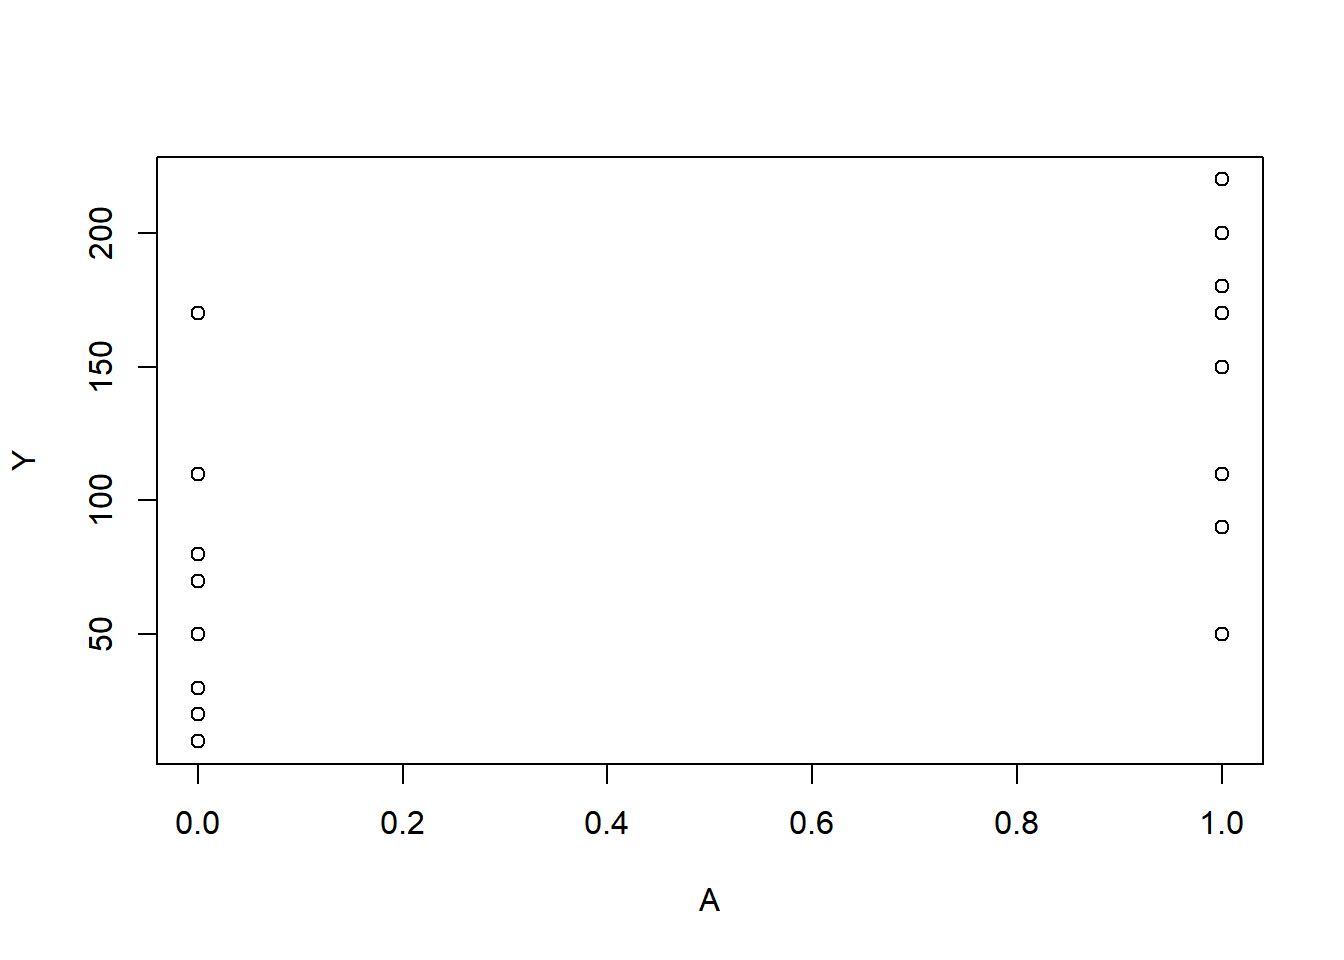
\includegraphics[width=0.85\linewidth]{11-why-model-r_files/figure-latex/unnamed-chunk-1-1} \end{center}

\begin{Shaded}
\begin{Highlighting}[]
\KeywordTok{summary}\NormalTok{(Y[A }\OperatorTok{==}\StringTok{ }\DecValTok{0}\NormalTok{])}
\end{Highlighting}
\end{Shaded}

\begin{verbatim}
##    Min. 1st Qu.  Median    Mean 3rd Qu.    Max. 
##    10.0    27.5    60.0    67.5    87.5   170.0
\end{verbatim}

\begin{Shaded}
\begin{Highlighting}[]
\KeywordTok{summary}\NormalTok{(Y[A }\OperatorTok{==}\StringTok{ }\DecValTok{1}\NormalTok{])}
\end{Highlighting}
\end{Shaded}

\begin{verbatim}
##    Min. 1st Qu.  Median    Mean 3rd Qu.    Max. 
##    50.0   105.0   160.0   146.2   185.0   220.0
\end{verbatim}

\begin{Shaded}
\begin{Highlighting}[]
\NormalTok{A2 <-}\StringTok{ }\KeywordTok{c}\NormalTok{(}\DecValTok{1}\NormalTok{, }\DecValTok{1}\NormalTok{, }\DecValTok{1}\NormalTok{, }\DecValTok{1}\NormalTok{, }\DecValTok{2}\NormalTok{, }\DecValTok{2}\NormalTok{, }\DecValTok{2}\NormalTok{, }\DecValTok{2}\NormalTok{, }\DecValTok{3}\NormalTok{, }\DecValTok{3}\NormalTok{, }\DecValTok{3}\NormalTok{, }\DecValTok{3}\NormalTok{, }\DecValTok{4}\NormalTok{, }\DecValTok{4}\NormalTok{, }\DecValTok{4}\NormalTok{, }\DecValTok{4}\NormalTok{)}
\NormalTok{Y2 <-}\StringTok{ }\KeywordTok{c}\NormalTok{(}\DecValTok{110}\NormalTok{, }\DecValTok{80}\NormalTok{, }\DecValTok{50}\NormalTok{, }\DecValTok{40}\NormalTok{, }\DecValTok{170}\NormalTok{, }\DecValTok{30}\NormalTok{, }\DecValTok{70}\NormalTok{, }\DecValTok{50}\NormalTok{, }\DecValTok{110}\NormalTok{, }\DecValTok{50}\NormalTok{, }\DecValTok{180}\NormalTok{,}
        \DecValTok{130}\NormalTok{, }\DecValTok{200}\NormalTok{, }\DecValTok{150}\NormalTok{, }\DecValTok{220}\NormalTok{, }\DecValTok{210}\NormalTok{)}

\KeywordTok{plot}\NormalTok{(A2, Y2)}
\end{Highlighting}
\end{Shaded}

\begin{center}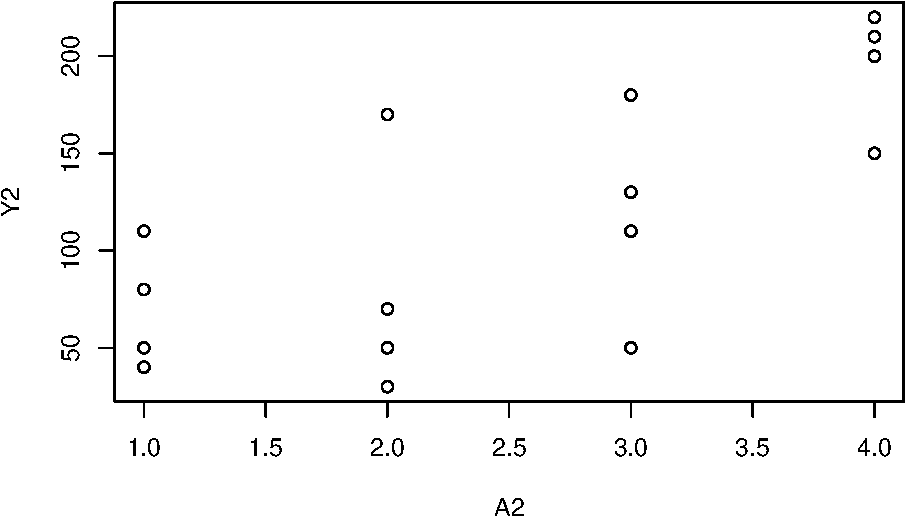
\includegraphics[width=0.85\linewidth]{11-why-model-r_files/figure-latex/unnamed-chunk-1-2} \end{center}

\begin{Shaded}
\begin{Highlighting}[]
\KeywordTok{summary}\NormalTok{(Y2[A2 }\OperatorTok{==}\StringTok{ }\DecValTok{1}\NormalTok{])}
\end{Highlighting}
\end{Shaded}

\begin{verbatim}
##    Min. 1st Qu.  Median    Mean 3rd Qu.    Max. 
##    40.0    47.5    65.0    70.0    87.5   110.0
\end{verbatim}

\begin{Shaded}
\begin{Highlighting}[]
\KeywordTok{summary}\NormalTok{(Y2[A2 }\OperatorTok{==}\StringTok{ }\DecValTok{2}\NormalTok{])}
\end{Highlighting}
\end{Shaded}

\begin{verbatim}
##    Min. 1st Qu.  Median    Mean 3rd Qu.    Max. 
##      30      45      60      80      95     170
\end{verbatim}

\begin{Shaded}
\begin{Highlighting}[]
\KeywordTok{summary}\NormalTok{(Y2[A2 }\OperatorTok{==}\StringTok{ }\DecValTok{3}\NormalTok{])}
\end{Highlighting}
\end{Shaded}

\begin{verbatim}
##    Min. 1st Qu.  Median    Mean 3rd Qu.    Max. 
##    50.0    95.0   120.0   117.5   142.5   180.0
\end{verbatim}

\begin{Shaded}
\begin{Highlighting}[]
\KeywordTok{summary}\NormalTok{(Y2[A2 }\OperatorTok{==}\StringTok{ }\DecValTok{4}\NormalTok{])}
\end{Highlighting}
\end{Shaded}

\begin{verbatim}
##    Min. 1st Qu.  Median    Mean 3rd Qu.    Max. 
##   150.0   187.5   205.0   195.0   212.5   220.0
\end{verbatim}

\hypertarget{program-11.2}{%
\section{Program 11.2}\label{program-11.2}}

\begin{itemize}
\tightlist
\item
  2-parameter linear model
\item
  Data from Figures 11.3 and 11.1
\end{itemize}

\begin{Shaded}
\begin{Highlighting}[]
\NormalTok{A3 <-}
\StringTok{  }\KeywordTok{c}\NormalTok{(}\DecValTok{3}\NormalTok{, }\DecValTok{11}\NormalTok{, }\DecValTok{17}\NormalTok{, }\DecValTok{23}\NormalTok{, }\DecValTok{29}\NormalTok{, }\DecValTok{37}\NormalTok{, }\DecValTok{41}\NormalTok{, }\DecValTok{53}\NormalTok{, }\DecValTok{67}\NormalTok{, }\DecValTok{79}\NormalTok{, }\DecValTok{83}\NormalTok{, }\DecValTok{97}\NormalTok{, }\DecValTok{60}\NormalTok{, }\DecValTok{71}\NormalTok{, }\DecValTok{15}\NormalTok{, }\DecValTok{45}\NormalTok{)}
\NormalTok{Y3 <-}
\StringTok{  }\KeywordTok{c}\NormalTok{(}\DecValTok{21}\NormalTok{, }\DecValTok{54}\NormalTok{, }\DecValTok{33}\NormalTok{, }\DecValTok{101}\NormalTok{, }\DecValTok{85}\NormalTok{, }\DecValTok{65}\NormalTok{, }\DecValTok{157}\NormalTok{, }\DecValTok{120}\NormalTok{, }\DecValTok{111}\NormalTok{, }\DecValTok{200}\NormalTok{, }\DecValTok{140}\NormalTok{, }\DecValTok{220}\NormalTok{, }\DecValTok{230}\NormalTok{, }\DecValTok{217}\NormalTok{,}
    \DecValTok{11}\NormalTok{, }\DecValTok{190}\NormalTok{)}

\KeywordTok{plot}\NormalTok{(Y3 }\OperatorTok{~}\StringTok{ }\NormalTok{A3)}
\end{Highlighting}
\end{Shaded}

\begin{center}\includegraphics[width=0.85\linewidth]{11-why-model-r_files/figure-latex/unnamed-chunk-2-1} \end{center}

\begin{Shaded}
\begin{Highlighting}[]
\KeywordTok{summary}\NormalTok{(}\KeywordTok{glm}\NormalTok{(Y3 }\OperatorTok{~}\StringTok{ }\NormalTok{A3))}
\end{Highlighting}
\end{Shaded}

\begin{verbatim}
## 
## Call:
## glm(formula = Y3 ~ A3)
## 
## Deviance Residuals: 
##     Min       1Q   Median       3Q      Max  
## -61.930  -30.564   -5.741   30.653   77.225  
## 
## Coefficients:
##             Estimate Std. Error t value Pr(>|t|)    
## (Intercept)  24.5464    21.3300   1.151 0.269094    
## A3            2.1372     0.3997   5.347 0.000103 ***
## ---
## Signif. codes:  0 '***' 0.001 '**' 0.01 '*' 0.05 '.' 0.1 ' ' 1
## 
## (Dispersion parameter for gaussian family taken to be 1944.109)
## 
##     Null deviance: 82800  on 15  degrees of freedom
## Residual deviance: 27218  on 14  degrees of freedom
## AIC: 170.43
## 
## Number of Fisher Scoring iterations: 2
\end{verbatim}

\begin{Shaded}
\begin{Highlighting}[]
\KeywordTok{predict}\NormalTok{(}\KeywordTok{glm}\NormalTok{(Y3 }\OperatorTok{~}\StringTok{ }\NormalTok{A3), }\KeywordTok{data.frame}\NormalTok{(}\DataTypeTok{A3 =} \DecValTok{90}\NormalTok{))}
\end{Highlighting}
\end{Shaded}

\begin{verbatim}
##      1 
## 216.89
\end{verbatim}

\begin{Shaded}
\begin{Highlighting}[]
\KeywordTok{summary}\NormalTok{(}\KeywordTok{glm}\NormalTok{(Y }\OperatorTok{~}\StringTok{ }\NormalTok{A))}
\end{Highlighting}
\end{Shaded}

\begin{verbatim}
## 
## Call:
## glm(formula = Y ~ A)
## 
## Deviance Residuals: 
##     Min       1Q   Median       3Q      Max  
## -96.250  -40.000    3.125   35.938  102.500  
## 
## Coefficients:
##             Estimate Std. Error t value Pr(>|t|)   
## (Intercept)    67.50      19.72   3.424  0.00412 **
## A              78.75      27.88   2.824  0.01352 * 
## ---
## Signif. codes:  0 '***' 0.001 '**' 0.01 '*' 0.05 '.' 0.1 ' ' 1
## 
## (Dispersion parameter for gaussian family taken to be 3109.821)
## 
##     Null deviance: 68344  on 15  degrees of freedom
## Residual deviance: 43538  on 14  degrees of freedom
## AIC: 177.95
## 
## Number of Fisher Scoring iterations: 2
\end{verbatim}

\hypertarget{program-11.3}{%
\section{Program 11.3}\label{program-11.3}}

\begin{itemize}
\tightlist
\item
  3-parameter linear model
\item
  Data from Figure 11.3
\end{itemize}

\begin{Shaded}
\begin{Highlighting}[]
\NormalTok{Asq <-}\StringTok{ }\NormalTok{A3 }\OperatorTok{*}\StringTok{ }\NormalTok{A3}

\NormalTok{mod3 <-}\StringTok{ }\KeywordTok{glm}\NormalTok{(Y3 }\OperatorTok{~}\StringTok{ }\NormalTok{A3 }\OperatorTok{+}\StringTok{ }\NormalTok{Asq)}
\KeywordTok{summary}\NormalTok{(mod3)}
\end{Highlighting}
\end{Shaded}

\begin{verbatim}
## 
## Call:
## glm(formula = Y3 ~ A3 + Asq)
## 
## Deviance Residuals: 
##    Min      1Q  Median      3Q     Max  
## -65.27  -34.41   13.21   26.11   64.36  
## 
## Coefficients:
##             Estimate Std. Error t value Pr(>|t|)  
## (Intercept) -7.40688   31.74777  -0.233   0.8192  
## A3           4.10723    1.53088   2.683   0.0188 *
## Asq         -0.02038    0.01532  -1.331   0.2062  
## ---
## Signif. codes:  0 '***' 0.001 '**' 0.01 '*' 0.05 '.' 0.1 ' ' 1
## 
## (Dispersion parameter for gaussian family taken to be 1842.697)
## 
##     Null deviance: 82800  on 15  degrees of freedom
## Residual deviance: 23955  on 13  degrees of freedom
## AIC: 170.39
## 
## Number of Fisher Scoring iterations: 2
\end{verbatim}

\begin{Shaded}
\begin{Highlighting}[]
\KeywordTok{predict}\NormalTok{(mod3, }\KeywordTok{data.frame}\NormalTok{(}\KeywordTok{cbind}\NormalTok{(}\DataTypeTok{A3 =} \DecValTok{90}\NormalTok{, }\DataTypeTok{Asq =} \DecValTok{8100}\NormalTok{)))}
\end{Highlighting}
\end{Shaded}

\begin{verbatim}
##        1 
## 197.1269
\end{verbatim}

\hypertarget{ip-weighting-and-marginal-structural-models}{%
\chapter*{12. IP Weighting and Marginal Structural Models}\label{ip-weighting-and-marginal-structural-models}}
\addcontentsline{toc}{chapter}{12. IP Weighting and Marginal Structural Models}

\hypertarget{program-12.1}{%
\section{Program 12.1}\label{program-12.1}}

\begin{itemize}
\tightlist
\item
  Descriptive statistics from NHEFS data (Table 12.1)
\end{itemize}

\begin{Shaded}
\begin{Highlighting}[]
\KeywordTok{library}\NormalTok{(here)}
\end{Highlighting}
\end{Shaded}

\begin{Shaded}
\begin{Highlighting}[]
\CommentTok{# install.packages("readxl") # install package if required}
\KeywordTok{library}\NormalTok{(}\StringTok{"readxl"}\NormalTok{)}

\NormalTok{nhefs <-}\StringTok{ }\KeywordTok{read_excel}\NormalTok{(}\KeywordTok{here}\NormalTok{(}\StringTok{"data"}\NormalTok{, }\StringTok{"NHEFS.xls"}\NormalTok{))}
\NormalTok{nhefs}\OperatorTok{$}\NormalTok{cens <-}\StringTok{ }\KeywordTok{ifelse}\NormalTok{(}\KeywordTok{is.na}\NormalTok{(nhefs}\OperatorTok{$}\NormalTok{wt82), }\DecValTok{1}\NormalTok{, }\DecValTok{0}\NormalTok{)}

\CommentTok{# provisionally ignore subjects with missing values for weight in 1982}
\NormalTok{nhefs.nmv <-}
\StringTok{  }\NormalTok{nhefs[}\KeywordTok{which}\NormalTok{(}\OperatorTok{!}\KeywordTok{is.na}\NormalTok{(nhefs}\OperatorTok{$}\NormalTok{wt82)),] }

\KeywordTok{lm}\NormalTok{(wt82_}\DecValTok{71} \OperatorTok{~}\StringTok{ }\NormalTok{qsmk, }\DataTypeTok{data =}\NormalTok{ nhefs.nmv)}
\end{Highlighting}
\end{Shaded}

\begin{verbatim}
## 
## Call:
## lm(formula = wt82_71 ~ qsmk, data = nhefs.nmv)
## 
## Coefficients:
## (Intercept)         qsmk  
##       1.984        2.541
\end{verbatim}

\begin{Shaded}
\begin{Highlighting}[]
\CommentTok{# Smoking cessation}
\KeywordTok{predict}\NormalTok{(}\KeywordTok{lm}\NormalTok{(wt82_}\DecValTok{71} \OperatorTok{~}\StringTok{ }\NormalTok{qsmk, }\DataTypeTok{data =}\NormalTok{ nhefs.nmv), }\KeywordTok{data.frame}\NormalTok{(}\DataTypeTok{qsmk =} \DecValTok{1}\NormalTok{))}
\end{Highlighting}
\end{Shaded}

\begin{verbatim}
##        1 
## 4.525079
\end{verbatim}

\begin{Shaded}
\begin{Highlighting}[]
\CommentTok{# No smoking cessation}
\KeywordTok{predict}\NormalTok{(}\KeywordTok{lm}\NormalTok{(wt82_}\DecValTok{71} \OperatorTok{~}\StringTok{ }\NormalTok{qsmk, }\DataTypeTok{data =}\NormalTok{ nhefs.nmv), }\KeywordTok{data.frame}\NormalTok{(}\DataTypeTok{qsmk =} \DecValTok{0}\NormalTok{)) }
\end{Highlighting}
\end{Shaded}

\begin{verbatim}
##        1 
## 1.984498
\end{verbatim}

\begin{Shaded}
\begin{Highlighting}[]
\CommentTok{# Table}
\KeywordTok{summary}\NormalTok{(nhefs.nmv[}\KeywordTok{which}\NormalTok{(nhefs.nmv}\OperatorTok{$}\NormalTok{qsmk }\OperatorTok{==}\StringTok{ }\DecValTok{0}\NormalTok{),]}\OperatorTok{$}\NormalTok{age)}
\end{Highlighting}
\end{Shaded}

\begin{verbatim}
##    Min. 1st Qu.  Median    Mean 3rd Qu.    Max. 
##   25.00   33.00   42.00   42.79   51.00   72.00
\end{verbatim}

\begin{Shaded}
\begin{Highlighting}[]
\KeywordTok{summary}\NormalTok{(nhefs.nmv[}\KeywordTok{which}\NormalTok{(nhefs.nmv}\OperatorTok{$}\NormalTok{qsmk }\OperatorTok{==}\StringTok{ }\DecValTok{0}\NormalTok{),]}\OperatorTok{$}\NormalTok{wt71)}
\end{Highlighting}
\end{Shaded}

\begin{verbatim}
##    Min. 1st Qu.  Median    Mean 3rd Qu.    Max. 
##   40.82   59.19   68.49   70.30   79.38  151.73
\end{verbatim}

\begin{Shaded}
\begin{Highlighting}[]
\KeywordTok{summary}\NormalTok{(nhefs.nmv[}\KeywordTok{which}\NormalTok{(nhefs.nmv}\OperatorTok{$}\NormalTok{qsmk }\OperatorTok{==}\StringTok{ }\DecValTok{0}\NormalTok{),]}\OperatorTok{$}\NormalTok{smokeintensity)}
\end{Highlighting}
\end{Shaded}

\begin{verbatim}
##    Min. 1st Qu.  Median    Mean 3rd Qu.    Max. 
##    1.00   15.00   20.00   21.19   30.00   60.00
\end{verbatim}

\begin{Shaded}
\begin{Highlighting}[]
\KeywordTok{summary}\NormalTok{(nhefs.nmv[}\KeywordTok{which}\NormalTok{(nhefs.nmv}\OperatorTok{$}\NormalTok{qsmk }\OperatorTok{==}\StringTok{ }\DecValTok{0}\NormalTok{),]}\OperatorTok{$}\NormalTok{smokeyrs)}
\end{Highlighting}
\end{Shaded}

\begin{verbatim}
##    Min. 1st Qu.  Median    Mean 3rd Qu.    Max. 
##    1.00   15.00   23.00   24.09   32.00   64.00
\end{verbatim}

\begin{Shaded}
\begin{Highlighting}[]
\KeywordTok{summary}\NormalTok{(nhefs.nmv[}\KeywordTok{which}\NormalTok{(nhefs.nmv}\OperatorTok{$}\NormalTok{qsmk }\OperatorTok{==}\StringTok{ }\DecValTok{1}\NormalTok{),]}\OperatorTok{$}\NormalTok{age)}
\end{Highlighting}
\end{Shaded}

\begin{verbatim}
##    Min. 1st Qu.  Median    Mean 3rd Qu.    Max. 
##   25.00   35.00   46.00   46.17   56.00   74.00
\end{verbatim}

\begin{Shaded}
\begin{Highlighting}[]
\KeywordTok{summary}\NormalTok{(nhefs.nmv[}\KeywordTok{which}\NormalTok{(nhefs.nmv}\OperatorTok{$}\NormalTok{qsmk }\OperatorTok{==}\StringTok{ }\DecValTok{1}\NormalTok{),]}\OperatorTok{$}\NormalTok{wt71)}
\end{Highlighting}
\end{Shaded}

\begin{verbatim}
##    Min. 1st Qu.  Median    Mean 3rd Qu.    Max. 
##   39.58   60.67   71.21   72.35   81.08  136.98
\end{verbatim}

\begin{Shaded}
\begin{Highlighting}[]
\KeywordTok{summary}\NormalTok{(nhefs.nmv[}\KeywordTok{which}\NormalTok{(nhefs.nmv}\OperatorTok{$}\NormalTok{qsmk }\OperatorTok{==}\StringTok{ }\DecValTok{1}\NormalTok{),]}\OperatorTok{$}\NormalTok{smokeintensity)}
\end{Highlighting}
\end{Shaded}

\begin{verbatim}
##    Min. 1st Qu.  Median    Mean 3rd Qu.    Max. 
##     1.0    10.0    20.0    18.6    25.0    80.0
\end{verbatim}

\begin{Shaded}
\begin{Highlighting}[]
\KeywordTok{summary}\NormalTok{(nhefs.nmv[}\KeywordTok{which}\NormalTok{(nhefs.nmv}\OperatorTok{$}\NormalTok{qsmk }\OperatorTok{==}\StringTok{ }\DecValTok{1}\NormalTok{),]}\OperatorTok{$}\NormalTok{smokeyrs)}
\end{Highlighting}
\end{Shaded}

\begin{verbatim}
##    Min. 1st Qu.  Median    Mean 3rd Qu.    Max. 
##    1.00   15.00   26.00   26.03   35.00   60.00
\end{verbatim}

\begin{Shaded}
\begin{Highlighting}[]
\KeywordTok{table}\NormalTok{(nhefs.nmv}\OperatorTok{$}\NormalTok{qsmk, nhefs.nmv}\OperatorTok{$}\NormalTok{sex)}
\end{Highlighting}
\end{Shaded}

\begin{verbatim}
##    
##       0   1
##   0 542 621
##   1 220 183
\end{verbatim}

\begin{Shaded}
\begin{Highlighting}[]
\KeywordTok{prop.table}\NormalTok{(}\KeywordTok{table}\NormalTok{(nhefs.nmv}\OperatorTok{$}\NormalTok{qsmk, nhefs.nmv}\OperatorTok{$}\NormalTok{sex), }\DecValTok{1}\NormalTok{)}
\end{Highlighting}
\end{Shaded}

\begin{verbatim}
##    
##             0         1
##   0 0.4660361 0.5339639
##   1 0.5459057 0.4540943
\end{verbatim}

\begin{Shaded}
\begin{Highlighting}[]
\KeywordTok{table}\NormalTok{(nhefs.nmv}\OperatorTok{$}\NormalTok{qsmk, nhefs.nmv}\OperatorTok{$}\NormalTok{race)}
\end{Highlighting}
\end{Shaded}

\begin{verbatim}
##    
##       0   1
##   0 993 170
##   1 367  36
\end{verbatim}

\begin{Shaded}
\begin{Highlighting}[]
\KeywordTok{prop.table}\NormalTok{(}\KeywordTok{table}\NormalTok{(nhefs.nmv}\OperatorTok{$}\NormalTok{qsmk, nhefs.nmv}\OperatorTok{$}\NormalTok{race), }\DecValTok{1}\NormalTok{)}
\end{Highlighting}
\end{Shaded}

\begin{verbatim}
##    
##              0          1
##   0 0.85382631 0.14617369
##   1 0.91066998 0.08933002
\end{verbatim}

\begin{Shaded}
\begin{Highlighting}[]
\KeywordTok{table}\NormalTok{(nhefs.nmv}\OperatorTok{$}\NormalTok{qsmk, nhefs.nmv}\OperatorTok{$}\NormalTok{education)}
\end{Highlighting}
\end{Shaded}

\begin{verbatim}
##    
##       1   2   3   4   5
##   0 210 266 480  92 115
##   1  81  74 157  29  62
\end{verbatim}

\begin{Shaded}
\begin{Highlighting}[]
\KeywordTok{prop.table}\NormalTok{(}\KeywordTok{table}\NormalTok{(nhefs.nmv}\OperatorTok{$}\NormalTok{qsmk, nhefs.nmv}\OperatorTok{$}\NormalTok{education), }\DecValTok{1}\NormalTok{)}
\end{Highlighting}
\end{Shaded}

\begin{verbatim}
##    
##              1          2          3          4          5
##   0 0.18056750 0.22871883 0.41272571 0.07910576 0.09888220
##   1 0.20099256 0.18362283 0.38957816 0.07196030 0.15384615
\end{verbatim}

\begin{Shaded}
\begin{Highlighting}[]
\KeywordTok{table}\NormalTok{(nhefs.nmv}\OperatorTok{$}\NormalTok{qsmk, nhefs.nmv}\OperatorTok{$}\NormalTok{exercise)}
\end{Highlighting}
\end{Shaded}

\begin{verbatim}
##    
##       0   1   2
##   0 237 485 441
##   1  63 176 164
\end{verbatim}

\begin{Shaded}
\begin{Highlighting}[]
\KeywordTok{prop.table}\NormalTok{(}\KeywordTok{table}\NormalTok{(nhefs.nmv}\OperatorTok{$}\NormalTok{qsmk, nhefs.nmv}\OperatorTok{$}\NormalTok{exercise), }\DecValTok{1}\NormalTok{)}
\end{Highlighting}
\end{Shaded}

\begin{verbatim}
##    
##             0         1         2
##   0 0.2037833 0.4170249 0.3791917
##   1 0.1563275 0.4367246 0.4069479
\end{verbatim}

\begin{Shaded}
\begin{Highlighting}[]
\KeywordTok{table}\NormalTok{(nhefs.nmv}\OperatorTok{$}\NormalTok{qsmk, nhefs.nmv}\OperatorTok{$}\NormalTok{active)}
\end{Highlighting}
\end{Shaded}

\begin{verbatim}
##    
##       0   1   2
##   0 532 527 104
##   1 170 188  45
\end{verbatim}

\begin{Shaded}
\begin{Highlighting}[]
\KeywordTok{prop.table}\NormalTok{(}\KeywordTok{table}\NormalTok{(nhefs.nmv}\OperatorTok{$}\NormalTok{qsmk, nhefs.nmv}\OperatorTok{$}\NormalTok{active), }\DecValTok{1}\NormalTok{)}
\end{Highlighting}
\end{Shaded}

\begin{verbatim}
##    
##             0         1         2
##   0 0.4574377 0.4531384 0.0894239
##   1 0.4218362 0.4665012 0.1116625
\end{verbatim}

\hypertarget{program-12.2}{%
\section{Program 12.2}\label{program-12.2}}

\begin{itemize}
\tightlist
\item
  Estimating IP weights
\item
  Data from NHEFS
\end{itemize}

\begin{Shaded}
\begin{Highlighting}[]
\CommentTok{# Estimation of ip weights via a logistic model}
\NormalTok{fit <-}\StringTok{ }\KeywordTok{glm}\NormalTok{(}
\NormalTok{  qsmk }\OperatorTok{~}\StringTok{ }\NormalTok{sex }\OperatorTok{+}\StringTok{ }\NormalTok{race }\OperatorTok{+}\StringTok{ }\NormalTok{age }\OperatorTok{+}\StringTok{ }\KeywordTok{I}\NormalTok{(age }\OperatorTok{^}\StringTok{ }\DecValTok{2}\NormalTok{) }\OperatorTok{+}
\StringTok{    }\KeywordTok{as.factor}\NormalTok{(education) }\OperatorTok{+}\StringTok{ }\NormalTok{smokeintensity }\OperatorTok{+}
\StringTok{    }\KeywordTok{I}\NormalTok{(smokeintensity }\OperatorTok{^}\StringTok{ }\DecValTok{2}\NormalTok{) }\OperatorTok{+}\StringTok{ }\NormalTok{smokeyrs }\OperatorTok{+}\StringTok{ }\KeywordTok{I}\NormalTok{(smokeyrs }\OperatorTok{^}\StringTok{ }\DecValTok{2}\NormalTok{) }\OperatorTok{+}
\StringTok{    }\KeywordTok{as.factor}\NormalTok{(exercise) }\OperatorTok{+}\StringTok{ }\KeywordTok{as.factor}\NormalTok{(active) }\OperatorTok{+}\StringTok{ }\NormalTok{wt71 }\OperatorTok{+}\StringTok{ }\KeywordTok{I}\NormalTok{(wt71 }\OperatorTok{^}\StringTok{ }\DecValTok{2}\NormalTok{),}
  \DataTypeTok{family =} \KeywordTok{binomial}\NormalTok{(),}
  \DataTypeTok{data =}\NormalTok{ nhefs.nmv}
\NormalTok{)}
\KeywordTok{summary}\NormalTok{(fit)}
\end{Highlighting}
\end{Shaded}

\begin{verbatim}
## 
## Call:
## glm(formula = qsmk ~ sex + race + age + I(age^2) + as.factor(education) + 
##     smokeintensity + I(smokeintensity^2) + smokeyrs + I(smokeyrs^2) + 
##     as.factor(exercise) + as.factor(active) + wt71 + I(wt71^2), 
##     family = binomial(), data = nhefs.nmv)
## 
## Deviance Residuals: 
##     Min       1Q   Median       3Q      Max  
## -1.5127  -0.7907  -0.6387   0.9832   2.3729  
## 
## Coefficients:
##                         Estimate Std. Error z value Pr(>|z|)    
## (Intercept)           -2.2425191  1.3808360  -1.624 0.104369    
## sex                   -0.5274782  0.1540496  -3.424 0.000617 ***
## race                  -0.8392636  0.2100665  -3.995 6.46e-05 ***
## age                    0.1212052  0.0512663   2.364 0.018068 *  
## I(age^2)              -0.0008246  0.0005361  -1.538 0.124039    
## as.factor(education)2 -0.0287755  0.1983506  -0.145 0.884653    
## as.factor(education)3  0.0864318  0.1780850   0.485 0.627435    
## as.factor(education)4  0.0636010  0.2732108   0.233 0.815924    
## as.factor(education)5  0.4759606  0.2262237   2.104 0.035384 *  
## smokeintensity        -0.0772704  0.0152499  -5.067 4.04e-07 ***
## I(smokeintensity^2)    0.0010451  0.0002866   3.647 0.000265 ***
## smokeyrs              -0.0735966  0.0277775  -2.650 0.008061 ** 
## I(smokeyrs^2)          0.0008441  0.0004632   1.822 0.068398 .  
## as.factor(exercise)1   0.3548405  0.1801351   1.970 0.048855 *  
## as.factor(exercise)2   0.3957040  0.1872400   2.113 0.034571 *  
## as.factor(active)1     0.0319445  0.1329372   0.240 0.810100    
## as.factor(active)2     0.1767840  0.2149720   0.822 0.410873    
## wt71                  -0.0152357  0.0263161  -0.579 0.562625    
## I(wt71^2)              0.0001352  0.0001632   0.829 0.407370    
## ---
## Signif. codes:  0 '***' 0.001 '**' 0.01 '*' 0.05 '.' 0.1 ' ' 1
## 
## (Dispersion parameter for binomial family taken to be 1)
## 
##     Null deviance: 1786.1  on 1565  degrees of freedom
## Residual deviance: 1676.9  on 1547  degrees of freedom
## AIC: 1714.9
## 
## Number of Fisher Scoring iterations: 4
\end{verbatim}

\begin{Shaded}
\begin{Highlighting}[]
\NormalTok{p.qsmk.obs <-}
\StringTok{  }\KeywordTok{ifelse}\NormalTok{(nhefs.nmv}\OperatorTok{$}\NormalTok{qsmk }\OperatorTok{==}\StringTok{ }\DecValTok{0}\NormalTok{,}
         \DecValTok{1} \OperatorTok{-}\StringTok{ }\KeywordTok{predict}\NormalTok{(fit, }\DataTypeTok{type =} \StringTok{"response"}\NormalTok{),}
         \KeywordTok{predict}\NormalTok{(fit, }\DataTypeTok{type =} \StringTok{"response"}\NormalTok{))}

\NormalTok{nhefs.nmv}\OperatorTok{$}\NormalTok{w <-}\StringTok{ }\DecValTok{1} \OperatorTok{/}\StringTok{ }\NormalTok{p.qsmk.obs}
\KeywordTok{summary}\NormalTok{(nhefs.nmv}\OperatorTok{$}\NormalTok{w)}
\end{Highlighting}
\end{Shaded}

\begin{verbatim}
##    Min. 1st Qu.  Median    Mean 3rd Qu.    Max. 
##   1.054   1.230   1.373   1.996   1.990  16.700
\end{verbatim}

\begin{Shaded}
\begin{Highlighting}[]
\KeywordTok{sd}\NormalTok{(nhefs.nmv}\OperatorTok{$}\NormalTok{w)}
\end{Highlighting}
\end{Shaded}

\begin{verbatim}
## [1] 1.474787
\end{verbatim}

\begin{Shaded}
\begin{Highlighting}[]
\CommentTok{# install.packages("geepack") # install package if required}
\KeywordTok{library}\NormalTok{(}\StringTok{"geepack"}\NormalTok{)}
\NormalTok{msm.w <-}\StringTok{ }\KeywordTok{geeglm}\NormalTok{(}
\NormalTok{  wt82_}\DecValTok{71} \OperatorTok{~}\StringTok{ }\NormalTok{qsmk,}
  \DataTypeTok{data =}\NormalTok{ nhefs.nmv,}
  \DataTypeTok{weights =}\NormalTok{ w,}
  \DataTypeTok{id =}\NormalTok{ seqn,}
  \DataTypeTok{corstr =} \StringTok{"independence"}
\NormalTok{)}
\KeywordTok{summary}\NormalTok{(msm.w)}
\end{Highlighting}
\end{Shaded}

\begin{verbatim}
## 
## Call:
## geeglm(formula = wt82_71 ~ qsmk, data = nhefs.nmv, weights = w, 
##     id = seqn, corstr = "independence")
## 
##  Coefficients:
##             Estimate Std.err  Wald Pr(>|W|)    
## (Intercept)   1.7800  0.2247 62.73 2.33e-15 ***
## qsmk          3.4405  0.5255 42.87 5.86e-11 ***
## ---
## Signif. codes:  0 '***' 0.001 '**' 0.01 '*' 0.05 '.' 0.1 ' ' 1
## 
## Estimated Scale Parameters:
##             Estimate Std.err
## (Intercept)    65.06   4.221
## 
## Correlation: Structure = independenceNumber of clusters:   1566   Maximum cluster size: 1
\end{verbatim}

\begin{Shaded}
\begin{Highlighting}[]
\NormalTok{beta <-}\StringTok{ }\KeywordTok{coef}\NormalTok{(msm.w)}
\NormalTok{SE <-}\StringTok{ }\KeywordTok{coef}\NormalTok{(}\KeywordTok{summary}\NormalTok{(msm.w))[, }\DecValTok{2}\NormalTok{]}
\NormalTok{lcl <-}\StringTok{ }\NormalTok{beta }\OperatorTok{-}\StringTok{ }\KeywordTok{qnorm}\NormalTok{(}\FloatTok{0.975}\NormalTok{) }\OperatorTok{*}\StringTok{ }\NormalTok{SE}
\NormalTok{ucl <-}\StringTok{ }\NormalTok{beta }\OperatorTok{+}\StringTok{ }\KeywordTok{qnorm}\NormalTok{(}\FloatTok{0.975}\NormalTok{) }\OperatorTok{*}\StringTok{ }\NormalTok{SE}
\KeywordTok{cbind}\NormalTok{(beta, lcl, ucl)}
\end{Highlighting}
\end{Shaded}

\begin{verbatim}
##              beta   lcl  ucl
## (Intercept) 1.780 1.340 2.22
## qsmk        3.441 2.411 4.47
\end{verbatim}

\begin{Shaded}
\begin{Highlighting}[]
\CommentTok{# no association between sex and qsmk in pseudo-population}
\KeywordTok{xtabs}\NormalTok{(nhefs.nmv}\OperatorTok{$}\NormalTok{w }\OperatorTok{~}\StringTok{ }\NormalTok{nhefs.nmv}\OperatorTok{$}\NormalTok{sex }\OperatorTok{+}\StringTok{ }\NormalTok{nhefs.nmv}\OperatorTok{$}\NormalTok{qsmk)}
\end{Highlighting}
\end{Shaded}

\begin{verbatim}
##              nhefs.nmv$qsmk
## nhefs.nmv$sex     0     1
##             0 763.6 763.6
##             1 801.7 797.2
\end{verbatim}

\begin{Shaded}
\begin{Highlighting}[]
\CommentTok{# "check" for positivity (White women)}
\KeywordTok{table}\NormalTok{(nhefs.nmv}\OperatorTok{$}\NormalTok{age[nhefs.nmv}\OperatorTok{$}\NormalTok{race }\OperatorTok{==}\StringTok{ }\DecValTok{0} \OperatorTok{&}\StringTok{ }\NormalTok{nhefs.nmv}\OperatorTok{$}\NormalTok{sex }\OperatorTok{==}\StringTok{ }\DecValTok{1}\NormalTok{],}
\NormalTok{      nhefs.nmv}\OperatorTok{$}\NormalTok{qsmk[nhefs.nmv}\OperatorTok{$}\NormalTok{race }\OperatorTok{==}\StringTok{ }\DecValTok{0} \OperatorTok{&}\StringTok{ }\NormalTok{nhefs.nmv}\OperatorTok{$}\NormalTok{sex }\OperatorTok{==}\StringTok{ }\DecValTok{1}\NormalTok{])}
\end{Highlighting}
\end{Shaded}

\begin{verbatim}
##     
##       0  1
##   25 24  3
##   26 14  5
##   27 18  2
##   28 20  5
##   29 15  4
##   30 14  5
##   31 11  5
##   32 14  7
##   33 12  3
##   34 22  5
##   35 16  5
##   36 13  3
##   37 14  1
##   38  6  2
##   39 19  4
##   40 10  4
##   41 13  3
##   42 16  3
##   43 14  3
##   44  9  4
##   45 12  5
##   46 19  4
##   47 19  4
##   48 19  4
##   49 11  3
##   50 18  4
##   51  9  3
##   52 11  3
##   53 11  4
##   54 17  9
##   55  9  4
##   56  8  7
##   57  9  2
##   58  8  4
##   59  5  4
##   60  5  4
##   61  5  2
##   62  6  5
##   63  3  3
##   64  7  1
##   65  3  2
##   66  4  0
##   67  2  0
##   69  6  2
##   70  2  1
##   71  0  1
##   72  2  2
##   74  0  1
\end{verbatim}

\hypertarget{program-12.3}{%
\section{Program 12.3}\label{program-12.3}}

\begin{itemize}
\tightlist
\item
  Estimating stabilized IP weights
\item
  Data from NHEFS
\end{itemize}

\begin{Shaded}
\begin{Highlighting}[]
\CommentTok{# estimation of denominator of ip weights}
\NormalTok{denom.fit <-}
\StringTok{  }\KeywordTok{glm}\NormalTok{(}
\NormalTok{    qsmk }\OperatorTok{~}\StringTok{ }\KeywordTok{as.factor}\NormalTok{(sex) }\OperatorTok{+}\StringTok{ }\KeywordTok{as.factor}\NormalTok{(race) }\OperatorTok{+}\StringTok{ }\NormalTok{age }\OperatorTok{+}\StringTok{ }\KeywordTok{I}\NormalTok{(age }\OperatorTok{^}\StringTok{ }\DecValTok{2}\NormalTok{) }\OperatorTok{+}
\StringTok{      }\KeywordTok{as.factor}\NormalTok{(education) }\OperatorTok{+}\StringTok{ }\NormalTok{smokeintensity }\OperatorTok{+}
\StringTok{      }\KeywordTok{I}\NormalTok{(smokeintensity }\OperatorTok{^}\StringTok{ }\DecValTok{2}\NormalTok{) }\OperatorTok{+}\StringTok{ }\NormalTok{smokeyrs }\OperatorTok{+}\StringTok{ }\KeywordTok{I}\NormalTok{(smokeyrs }\OperatorTok{^}\StringTok{ }\DecValTok{2}\NormalTok{) }\OperatorTok{+}
\StringTok{      }\KeywordTok{as.factor}\NormalTok{(exercise) }\OperatorTok{+}\StringTok{ }\KeywordTok{as.factor}\NormalTok{(active) }\OperatorTok{+}\StringTok{ }\NormalTok{wt71 }\OperatorTok{+}\StringTok{ }\KeywordTok{I}\NormalTok{(wt71 }\OperatorTok{^}\StringTok{ }\DecValTok{2}\NormalTok{),}
    \DataTypeTok{family =} \KeywordTok{binomial}\NormalTok{(),}
    \DataTypeTok{data =}\NormalTok{ nhefs.nmv}
\NormalTok{  )}
\KeywordTok{summary}\NormalTok{(denom.fit)}
\end{Highlighting}
\end{Shaded}

\begin{verbatim}
## 
## Call:
## glm(formula = qsmk ~ as.factor(sex) + as.factor(race) + age + 
##     I(age^2) + as.factor(education) + smokeintensity + I(smokeintensity^2) + 
##     smokeyrs + I(smokeyrs^2) + as.factor(exercise) + as.factor(active) + 
##     wt71 + I(wt71^2), family = binomial(), data = nhefs.nmv)
## 
## Deviance Residuals: 
##    Min      1Q  Median      3Q     Max  
## -1.513  -0.791  -0.639   0.983   2.373  
## 
## Coefficients:
##                        Estimate Std. Error z value Pr(>|z|)    
## (Intercept)           -2.242519   1.380836   -1.62  0.10437    
## as.factor(sex)1       -0.527478   0.154050   -3.42  0.00062 ***
## as.factor(race)1      -0.839264   0.210067   -4.00  6.5e-05 ***
## age                    0.121205   0.051266    2.36  0.01807 *  
## I(age^2)              -0.000825   0.000536   -1.54  0.12404    
## as.factor(education)2 -0.028776   0.198351   -0.15  0.88465    
## as.factor(education)3  0.086432   0.178085    0.49  0.62744    
## as.factor(education)4  0.063601   0.273211    0.23  0.81592    
## as.factor(education)5  0.475961   0.226224    2.10  0.03538 *  
## smokeintensity        -0.077270   0.015250   -5.07  4.0e-07 ***
## I(smokeintensity^2)    0.001045   0.000287    3.65  0.00027 ***
## smokeyrs              -0.073597   0.027777   -2.65  0.00806 ** 
## I(smokeyrs^2)          0.000844   0.000463    1.82  0.06840 .  
## as.factor(exercise)1   0.354841   0.180135    1.97  0.04885 *  
## as.factor(exercise)2   0.395704   0.187240    2.11  0.03457 *  
## as.factor(active)1     0.031944   0.132937    0.24  0.81010    
## as.factor(active)2     0.176784   0.214972    0.82  0.41087    
## wt71                  -0.015236   0.026316   -0.58  0.56262    
## I(wt71^2)              0.000135   0.000163    0.83  0.40737    
## ---
## Signif. codes:  0 '***' 0.001 '**' 0.01 '*' 0.05 '.' 0.1 ' ' 1
## 
## (Dispersion parameter for binomial family taken to be 1)
## 
##     Null deviance: 1786.1  on 1565  degrees of freedom
## Residual deviance: 1676.9  on 1547  degrees of freedom
## AIC: 1715
## 
## Number of Fisher Scoring iterations: 4
\end{verbatim}

\begin{Shaded}
\begin{Highlighting}[]
\NormalTok{pd.qsmk <-}\StringTok{ }\KeywordTok{predict}\NormalTok{(denom.fit, }\DataTypeTok{type =} \StringTok{"response"}\NormalTok{)}

\CommentTok{# estimation of numerator of ip weights}
\NormalTok{numer.fit <-}\StringTok{ }\KeywordTok{glm}\NormalTok{(qsmk }\OperatorTok{~}\StringTok{ }\DecValTok{1}\NormalTok{, }\DataTypeTok{family =} \KeywordTok{binomial}\NormalTok{(), }\DataTypeTok{data =}\NormalTok{ nhefs.nmv)}
\KeywordTok{summary}\NormalTok{(numer.fit)}
\end{Highlighting}
\end{Shaded}

\begin{verbatim}
## 
## Call:
## glm(formula = qsmk ~ 1, family = binomial(), data = nhefs.nmv)
## 
## Deviance Residuals: 
##    Min      1Q  Median      3Q     Max  
## -0.771  -0.771  -0.771   1.648   1.648  
## 
## Coefficients:
##             Estimate Std. Error z value Pr(>|z|)    
## (Intercept)  -1.0598     0.0578   -18.3   <2e-16 ***
## ---
## Signif. codes:  0 '***' 0.001 '**' 0.01 '*' 0.05 '.' 0.1 ' ' 1
## 
## (Dispersion parameter for binomial family taken to be 1)
## 
##     Null deviance: 1786.1  on 1565  degrees of freedom
## Residual deviance: 1786.1  on 1565  degrees of freedom
## AIC: 1788
## 
## Number of Fisher Scoring iterations: 4
\end{verbatim}

\begin{Shaded}
\begin{Highlighting}[]
\NormalTok{pn.qsmk <-}\StringTok{ }\KeywordTok{predict}\NormalTok{(numer.fit, }\DataTypeTok{type =} \StringTok{"response"}\NormalTok{)}

\NormalTok{nhefs.nmv}\OperatorTok{$}\NormalTok{sw <-}
\StringTok{  }\KeywordTok{ifelse}\NormalTok{(nhefs.nmv}\OperatorTok{$}\NormalTok{qsmk }\OperatorTok{==}\StringTok{ }\DecValTok{0}\NormalTok{, ((}\DecValTok{1} \OperatorTok{-}\StringTok{ }\NormalTok{pn.qsmk) }\OperatorTok{/}\StringTok{ }\NormalTok{(}\DecValTok{1} \OperatorTok{-}\StringTok{ }\NormalTok{pd.qsmk)),}
\NormalTok{         (pn.qsmk }\OperatorTok{/}\StringTok{ }\NormalTok{pd.qsmk))}

\KeywordTok{summary}\NormalTok{(nhefs.nmv}\OperatorTok{$}\NormalTok{sw)}
\end{Highlighting}
\end{Shaded}

\begin{verbatim}
##    Min. 1st Qu.  Median    Mean 3rd Qu.    Max. 
##   0.331   0.867   0.950   0.999   1.079   4.298
\end{verbatim}

\begin{Shaded}
\begin{Highlighting}[]
\NormalTok{msm.sw <-}\StringTok{ }\KeywordTok{geeglm}\NormalTok{(}
\NormalTok{  wt82_}\DecValTok{71} \OperatorTok{~}\StringTok{ }\NormalTok{qsmk,}
  \DataTypeTok{data =}\NormalTok{ nhefs.nmv,}
  \DataTypeTok{weights =}\NormalTok{ sw,}
  \DataTypeTok{id =}\NormalTok{ seqn,}
  \DataTypeTok{corstr =} \StringTok{"independence"}
\NormalTok{)}
\KeywordTok{summary}\NormalTok{(msm.sw)}
\end{Highlighting}
\end{Shaded}

\begin{verbatim}
## 
## Call:
## geeglm(formula = wt82_71 ~ qsmk, data = nhefs.nmv, weights = sw, 
##     id = seqn, corstr = "independence")
## 
##  Coefficients:
##             Estimate Std.err Wald Pr(>|W|)    
## (Intercept)    1.780   0.225 62.7  2.3e-15 ***
## qsmk           3.441   0.525 42.9  5.9e-11 ***
## ---
## Signif. codes:  0 '***' 0.001 '**' 0.01 '*' 0.05 '.' 0.1 ' ' 1
## 
## Estimated Scale Parameters:
##             Estimate Std.err
## (Intercept)     60.7    3.71
## 
## Correlation: Structure = independenceNumber of clusters:   1566   Maximum cluster size: 1
\end{verbatim}

\begin{Shaded}
\begin{Highlighting}[]
\NormalTok{beta <-}\StringTok{ }\KeywordTok{coef}\NormalTok{(msm.sw)}
\NormalTok{SE <-}\StringTok{ }\KeywordTok{coef}\NormalTok{(}\KeywordTok{summary}\NormalTok{(msm.sw))[, }\DecValTok{2}\NormalTok{]}
\NormalTok{lcl <-}\StringTok{ }\NormalTok{beta }\OperatorTok{-}\StringTok{ }\KeywordTok{qnorm}\NormalTok{(}\FloatTok{0.975}\NormalTok{) }\OperatorTok{*}\StringTok{ }\NormalTok{SE}
\NormalTok{ucl <-}\StringTok{ }\NormalTok{beta }\OperatorTok{+}\StringTok{ }\KeywordTok{qnorm}\NormalTok{(}\FloatTok{0.975}\NormalTok{) }\OperatorTok{*}\StringTok{ }\NormalTok{SE}
\KeywordTok{cbind}\NormalTok{(beta, lcl, ucl)}
\end{Highlighting}
\end{Shaded}

\begin{verbatim}
##             beta  lcl  ucl
## (Intercept) 1.78 1.34 2.22
## qsmk        3.44 2.41 4.47
\end{verbatim}

\begin{Shaded}
\begin{Highlighting}[]
\CommentTok{# no association between sex and qsmk in pseudo-population}
\KeywordTok{xtabs}\NormalTok{(nhefs.nmv}\OperatorTok{$}\NormalTok{sw }\OperatorTok{~}\StringTok{ }\NormalTok{nhefs.nmv}\OperatorTok{$}\NormalTok{sex }\OperatorTok{+}\StringTok{ }\NormalTok{nhefs.nmv}\OperatorTok{$}\NormalTok{qsmk)}
\end{Highlighting}
\end{Shaded}

\begin{verbatim}
##              nhefs.nmv$qsmk
## nhefs.nmv$sex   0   1
##             0 567 197
##             1 595 205
\end{verbatim}

\hypertarget{program-12.4}{%
\section{Program 12.4}\label{program-12.4}}

\begin{itemize}
\tightlist
\item
  Estimating the parameters of a marginal structural mean model with a continuous treatment Data from NHEFS
\end{itemize}

\begin{Shaded}
\begin{Highlighting}[]
\CommentTok{# Analysis restricted to subjects reporting <=25 cig/day at baseline}
\NormalTok{nhefs.nmv.s <-}\StringTok{ }\KeywordTok{subset}\NormalTok{(nhefs.nmv, smokeintensity }\OperatorTok{<=}\StringTok{ }\DecValTok{25}\NormalTok{)}

\CommentTok{# estimation of denominator of ip weights}
\NormalTok{den.fit.obj <-}\StringTok{ }\KeywordTok{lm}\NormalTok{(}
\NormalTok{  smkintensity82_}\DecValTok{71} \OperatorTok{~}\StringTok{ }\KeywordTok{as.factor}\NormalTok{(sex) }\OperatorTok{+}
\StringTok{    }\KeywordTok{as.factor}\NormalTok{(race) }\OperatorTok{+}\StringTok{ }\NormalTok{age }\OperatorTok{+}\StringTok{ }\KeywordTok{I}\NormalTok{(age }\OperatorTok{^}\StringTok{ }\DecValTok{2}\NormalTok{) }\OperatorTok{+}
\StringTok{    }\KeywordTok{as.factor}\NormalTok{(education) }\OperatorTok{+}\StringTok{ }\NormalTok{smokeintensity }\OperatorTok{+}\StringTok{ }\KeywordTok{I}\NormalTok{(smokeintensity }\OperatorTok{^}\StringTok{ }\DecValTok{2}\NormalTok{) }\OperatorTok{+}
\StringTok{    }\NormalTok{smokeyrs }\OperatorTok{+}\StringTok{ }\KeywordTok{I}\NormalTok{(smokeyrs }\OperatorTok{^}\StringTok{ }\DecValTok{2}\NormalTok{) }\OperatorTok{+}\StringTok{ }\KeywordTok{as.factor}\NormalTok{(exercise) }\OperatorTok{+}\StringTok{ }\KeywordTok{as.factor}\NormalTok{(active) }\OperatorTok{+}\StringTok{ }\NormalTok{wt71 }\OperatorTok{+}
\StringTok{    }\KeywordTok{I}\NormalTok{(wt71 }\OperatorTok{^}\StringTok{ }\DecValTok{2}\NormalTok{),}
  \DataTypeTok{data =}\NormalTok{ nhefs.nmv.s}
\NormalTok{)}
\NormalTok{p.den <-}\StringTok{ }\KeywordTok{predict}\NormalTok{(den.fit.obj, }\DataTypeTok{type =} \StringTok{"response"}\NormalTok{)}
\NormalTok{dens.den <-}
\StringTok{  }\KeywordTok{dnorm}\NormalTok{(nhefs.nmv.s}\OperatorTok{$}\NormalTok{smkintensity82_}\DecValTok{71}\NormalTok{,}
\NormalTok{        p.den,}
        \KeywordTok{summary}\NormalTok{(den.fit.obj)}\OperatorTok{$}\NormalTok{sigma)}

\CommentTok{# estimation of numerator of ip weights}
\NormalTok{num.fit.obj <-}\StringTok{ }\KeywordTok{lm}\NormalTok{(smkintensity82_}\DecValTok{71} \OperatorTok{~}\StringTok{ }\DecValTok{1}\NormalTok{, }\DataTypeTok{data =}\NormalTok{ nhefs.nmv.s)}
\NormalTok{p.num <-}\StringTok{ }\KeywordTok{predict}\NormalTok{(num.fit.obj, }\DataTypeTok{type =} \StringTok{"response"}\NormalTok{)}
\NormalTok{dens.num <-}
\StringTok{  }\KeywordTok{dnorm}\NormalTok{(nhefs.nmv.s}\OperatorTok{$}\NormalTok{smkintensity82_}\DecValTok{71}\NormalTok{,}
\NormalTok{        p.num,}
        \KeywordTok{summary}\NormalTok{(num.fit.obj)}\OperatorTok{$}\NormalTok{sigma)}

\NormalTok{nhefs.nmv.s}\OperatorTok{$}\NormalTok{sw.a <-}\StringTok{ }\NormalTok{dens.num }\OperatorTok{/}\StringTok{ }\NormalTok{dens.den}
\KeywordTok{summary}\NormalTok{(nhefs.nmv.s}\OperatorTok{$}\NormalTok{sw.a)}
\end{Highlighting}
\end{Shaded}

\begin{verbatim}
##    Min. 1st Qu.  Median    Mean 3rd Qu.    Max. 
##    0.19    0.89    0.97    1.00    1.05    5.10
\end{verbatim}

\begin{Shaded}
\begin{Highlighting}[]
\NormalTok{msm.sw.cont <-}
\StringTok{  }\KeywordTok{geeglm}\NormalTok{(}
\NormalTok{    wt82_}\DecValTok{71} \OperatorTok{~}\StringTok{ }\NormalTok{smkintensity82_}\DecValTok{71} \OperatorTok{+}\StringTok{ }\KeywordTok{I}\NormalTok{(smkintensity82_}\DecValTok{71} \OperatorTok{*}\StringTok{ }\NormalTok{smkintensity82_}\DecValTok{71}\NormalTok{),}
    \DataTypeTok{data =}\NormalTok{ nhefs.nmv.s,}
    \DataTypeTok{weights =}\NormalTok{ sw.a,}
    \DataTypeTok{id =}\NormalTok{ seqn,}
    \DataTypeTok{corstr =} \StringTok{"independence"}
\NormalTok{  )}
\KeywordTok{summary}\NormalTok{(msm.sw.cont)}
\end{Highlighting}
\end{Shaded}

\begin{verbatim}
## 
## Call:
## geeglm(formula = wt82_71 ~ smkintensity82_71 + I(smkintensity82_71 * 
##     smkintensity82_71), data = nhefs.nmv.s, weights = sw.a, id = seqn, 
##     corstr = "independence")
## 
##  Coefficients:
##                                          Estimate  Std.err  Wald Pr(>|W|)
## (Intercept)                               2.00452  0.29512 46.13  1.1e-11
## smkintensity82_71                        -0.10899  0.03154 11.94  0.00055
## I(smkintensity82_71 * smkintensity82_71)  0.00269  0.00242  1.24  0.26489
##                                             
## (Intercept)                              ***
## smkintensity82_71                        ***
## I(smkintensity82_71 * smkintensity82_71)    
## ---
## Signif. codes:  0 '***' 0.001 '**' 0.01 '*' 0.05 '.' 0.1 ' ' 1
## 
## Estimated Scale Parameters:
##             Estimate Std.err
## (Intercept)     60.5     4.5
## 
## Correlation: Structure = independenceNumber of clusters:   1162   Maximum cluster size: 1
\end{verbatim}

\begin{Shaded}
\begin{Highlighting}[]
\NormalTok{beta <-}\StringTok{ }\KeywordTok{coef}\NormalTok{(msm.sw.cont)}
\NormalTok{SE <-}\StringTok{ }\KeywordTok{coef}\NormalTok{(}\KeywordTok{summary}\NormalTok{(msm.sw.cont))[, }\DecValTok{2}\NormalTok{]}
\NormalTok{lcl <-}\StringTok{ }\NormalTok{beta }\OperatorTok{-}\StringTok{ }\KeywordTok{qnorm}\NormalTok{(}\FloatTok{0.975}\NormalTok{) }\OperatorTok{*}\StringTok{ }\NormalTok{SE}
\NormalTok{ucl <-}\StringTok{ }\NormalTok{beta }\OperatorTok{+}\StringTok{ }\KeywordTok{qnorm}\NormalTok{(}\FloatTok{0.975}\NormalTok{) }\OperatorTok{*}\StringTok{ }\NormalTok{SE}
\KeywordTok{cbind}\NormalTok{(beta, lcl, ucl)}
\end{Highlighting}
\end{Shaded}

\begin{verbatim}
##                                              beta      lcl      ucl
## (Intercept)                               2.00452  1.42610  2.58295
## smkintensity82_71                        -0.10899 -0.17080 -0.04718
## I(smkintensity82_71 * smkintensity82_71)  0.00269 -0.00204  0.00743
\end{verbatim}

\hypertarget{program-12.5}{%
\section{Program 12.5}\label{program-12.5}}

\begin{itemize}
\tightlist
\item
  Estimating the parameters of a marginal structural logistic model
\item
  Data from NHEFS
\end{itemize}

\begin{Shaded}
\begin{Highlighting}[]
\KeywordTok{table}\NormalTok{(nhefs.nmv}\OperatorTok{$}\NormalTok{qsmk, nhefs.nmv}\OperatorTok{$}\NormalTok{death)}
\end{Highlighting}
\end{Shaded}

\begin{verbatim}
##    
##       0   1
##   0 963 200
##   1 312  91
\end{verbatim}

\begin{Shaded}
\begin{Highlighting}[]
\CommentTok{# First, estimation of stabilized weights sw (same as in Program 12.3)}
\CommentTok{# Second, fit logistic model below}
\NormalTok{msm.logistic <-}\StringTok{ }\KeywordTok{geeglm}\NormalTok{(}
\NormalTok{  death }\OperatorTok{~}\StringTok{ }\NormalTok{qsmk,}
  \DataTypeTok{data =}\NormalTok{ nhefs.nmv,}
  \DataTypeTok{weights =}\NormalTok{ sw,}
  \DataTypeTok{id =}\NormalTok{ seqn,}
  \DataTypeTok{family =} \KeywordTok{binomial}\NormalTok{(),}
  \DataTypeTok{corstr =} \StringTok{"independence"}
\NormalTok{)}
\end{Highlighting}
\end{Shaded}

\begin{verbatim}
## Warning in eval(family$initialize): non-integer #successes in a binomial
## glm!
\end{verbatim}

\begin{Shaded}
\begin{Highlighting}[]
\KeywordTok{summary}\NormalTok{(msm.logistic)}
\end{Highlighting}
\end{Shaded}

\begin{verbatim}
## 
## Call:
## geeglm(formula = death ~ qsmk, family = binomial(), data = nhefs.nmv, 
##     weights = sw, id = seqn, corstr = "independence")
## 
##  Coefficients:
##             Estimate Std.err   Wald Pr(>|W|)    
## (Intercept)  -1.4905  0.0789 356.50   <2e-16 ***
## qsmk          0.0301  0.1573   0.04     0.85    
## ---
## Signif. codes:  0 '***' 0.001 '**' 0.01 '*' 0.05 '.' 0.1 ' ' 1
## 
## Estimated Scale Parameters:
##             Estimate Std.err
## (Intercept)        1  0.0678
## 
## Correlation: Structure = independenceNumber of clusters:   1566   Maximum cluster size: 1
\end{verbatim}

\begin{Shaded}
\begin{Highlighting}[]
\NormalTok{beta <-}\StringTok{ }\KeywordTok{coef}\NormalTok{(msm.logistic)}
\NormalTok{SE <-}\StringTok{ }\KeywordTok{coef}\NormalTok{(}\KeywordTok{summary}\NormalTok{(msm.logistic))[, }\DecValTok{2}\NormalTok{]}
\NormalTok{lcl <-}\StringTok{ }\NormalTok{beta }\OperatorTok{-}\StringTok{ }\KeywordTok{qnorm}\NormalTok{(}\FloatTok{0.975}\NormalTok{) }\OperatorTok{*}\StringTok{ }\NormalTok{SE}
\NormalTok{ucl <-}\StringTok{ }\NormalTok{beta }\OperatorTok{+}\StringTok{ }\KeywordTok{qnorm}\NormalTok{(}\FloatTok{0.975}\NormalTok{) }\OperatorTok{*}\StringTok{ }\NormalTok{SE}
\KeywordTok{cbind}\NormalTok{(beta, lcl, ucl)}
\end{Highlighting}
\end{Shaded}

\begin{verbatim}
##                beta    lcl    ucl
## (Intercept) -1.4905 -1.645 -1.336
## qsmk         0.0301 -0.278  0.338
\end{verbatim}

\hypertarget{program-12.6}{%
\section{Program 12.6}\label{program-12.6}}

\begin{itemize}
\tightlist
\item
  Assessing effect modification by sex using a marginal structural mean model
\item
  Data from NHEFS
\end{itemize}

\begin{Shaded}
\begin{Highlighting}[]
\KeywordTok{table}\NormalTok{(nhefs.nmv}\OperatorTok{$}\NormalTok{sex)}
\end{Highlighting}
\end{Shaded}

\begin{verbatim}
## 
##   0   1 
## 762 804
\end{verbatim}

\begin{Shaded}
\begin{Highlighting}[]
\CommentTok{# estimation of denominator of ip weights}
\NormalTok{denom.fit <-}
\StringTok{  }\KeywordTok{glm}\NormalTok{(}
\NormalTok{    qsmk }\OperatorTok{~}\StringTok{ }\KeywordTok{as.factor}\NormalTok{(sex) }\OperatorTok{+}\StringTok{ }\KeywordTok{as.factor}\NormalTok{(race) }\OperatorTok{+}\StringTok{ }\NormalTok{age }\OperatorTok{+}\StringTok{ }\KeywordTok{I}\NormalTok{(age }\OperatorTok{^}\StringTok{ }\DecValTok{2}\NormalTok{) }\OperatorTok{+}
\StringTok{      }\KeywordTok{as.factor}\NormalTok{(education) }\OperatorTok{+}\StringTok{ }\NormalTok{smokeintensity }\OperatorTok{+}
\StringTok{      }\KeywordTok{I}\NormalTok{(smokeintensity }\OperatorTok{^}\StringTok{ }\DecValTok{2}\NormalTok{) }\OperatorTok{+}\StringTok{ }\NormalTok{smokeyrs }\OperatorTok{+}\StringTok{ }\KeywordTok{I}\NormalTok{(smokeyrs }\OperatorTok{^}\StringTok{ }\DecValTok{2}\NormalTok{) }\OperatorTok{+}
\StringTok{      }\KeywordTok{as.factor}\NormalTok{(exercise) }\OperatorTok{+}\StringTok{ }\KeywordTok{as.factor}\NormalTok{(active) }\OperatorTok{+}\StringTok{ }\NormalTok{wt71 }\OperatorTok{+}\StringTok{ }\KeywordTok{I}\NormalTok{(wt71 }\OperatorTok{^}\StringTok{ }\DecValTok{2}\NormalTok{),}
    \DataTypeTok{family =} \KeywordTok{binomial}\NormalTok{(),}
    \DataTypeTok{data =}\NormalTok{ nhefs.nmv}
\NormalTok{  )}
\KeywordTok{summary}\NormalTok{(denom.fit)}
\end{Highlighting}
\end{Shaded}

\begin{verbatim}
## 
## Call:
## glm(formula = qsmk ~ as.factor(sex) + as.factor(race) + age + 
##     I(age^2) + as.factor(education) + smokeintensity + I(smokeintensity^2) + 
##     smokeyrs + I(smokeyrs^2) + as.factor(exercise) + as.factor(active) + 
##     wt71 + I(wt71^2), family = binomial(), data = nhefs.nmv)
## 
## Deviance Residuals: 
##    Min      1Q  Median      3Q     Max  
## -1.513  -0.791  -0.639   0.983   2.373  
## 
## Coefficients:
##                        Estimate Std. Error z value Pr(>|z|)    
## (Intercept)           -2.242519   1.380836   -1.62  0.10437    
## as.factor(sex)1       -0.527478   0.154050   -3.42  0.00062 ***
## as.factor(race)1      -0.839264   0.210067   -4.00  6.5e-05 ***
## age                    0.121205   0.051266    2.36  0.01807 *  
## I(age^2)              -0.000825   0.000536   -1.54  0.12404    
## as.factor(education)2 -0.028776   0.198351   -0.15  0.88465    
## as.factor(education)3  0.086432   0.178085    0.49  0.62744    
## as.factor(education)4  0.063601   0.273211    0.23  0.81592    
## as.factor(education)5  0.475961   0.226224    2.10  0.03538 *  
## smokeintensity        -0.077270   0.015250   -5.07  4.0e-07 ***
## I(smokeintensity^2)    0.001045   0.000287    3.65  0.00027 ***
## smokeyrs              -0.073597   0.027777   -2.65  0.00806 ** 
## I(smokeyrs^2)          0.000844   0.000463    1.82  0.06840 .  
## as.factor(exercise)1   0.354841   0.180135    1.97  0.04885 *  
## as.factor(exercise)2   0.395704   0.187240    2.11  0.03457 *  
## as.factor(active)1     0.031944   0.132937    0.24  0.81010    
## as.factor(active)2     0.176784   0.214972    0.82  0.41087    
## wt71                  -0.015236   0.026316   -0.58  0.56262    
## I(wt71^2)              0.000135   0.000163    0.83  0.40737    
## ---
## Signif. codes:  0 '***' 0.001 '**' 0.01 '*' 0.05 '.' 0.1 ' ' 1
## 
## (Dispersion parameter for binomial family taken to be 1)
## 
##     Null deviance: 1786.1  on 1565  degrees of freedom
## Residual deviance: 1676.9  on 1547  degrees of freedom
## AIC: 1715
## 
## Number of Fisher Scoring iterations: 4
\end{verbatim}

\begin{Shaded}
\begin{Highlighting}[]
\NormalTok{pd.qsmk <-}\StringTok{ }\KeywordTok{predict}\NormalTok{(denom.fit, }\DataTypeTok{type =} \StringTok{"response"}\NormalTok{)}

\CommentTok{# estimation of numerator of ip weights}
\NormalTok{numer.fit <-}
\StringTok{  }\KeywordTok{glm}\NormalTok{(qsmk }\OperatorTok{~}\StringTok{ }\KeywordTok{as.factor}\NormalTok{(sex), }\DataTypeTok{family =} \KeywordTok{binomial}\NormalTok{(), }\DataTypeTok{data =}\NormalTok{ nhefs.nmv)}
\KeywordTok{summary}\NormalTok{(numer.fit)}
\end{Highlighting}
\end{Shaded}

\begin{verbatim}
## 
## Call:
## glm(formula = qsmk ~ as.factor(sex), family = binomial(), data = nhefs.nmv)
## 
## Deviance Residuals: 
##    Min      1Q  Median      3Q     Max  
## -0.825  -0.825  -0.719   1.576   1.720  
## 
## Coefficients:
##                 Estimate Std. Error z value Pr(>|z|)    
## (Intercept)      -0.9016     0.0799  -11.28   <2e-16 ***
## as.factor(sex)1  -0.3202     0.1160   -2.76   0.0058 ** 
## ---
## Signif. codes:  0 '***' 0.001 '**' 0.01 '*' 0.05 '.' 0.1 ' ' 1
## 
## (Dispersion parameter for binomial family taken to be 1)
## 
##     Null deviance: 1786.1  on 1565  degrees of freedom
## Residual deviance: 1778.4  on 1564  degrees of freedom
## AIC: 1782
## 
## Number of Fisher Scoring iterations: 4
\end{verbatim}

\begin{Shaded}
\begin{Highlighting}[]
\NormalTok{pn.qsmk <-}\StringTok{ }\KeywordTok{predict}\NormalTok{(numer.fit, }\DataTypeTok{type =} \StringTok{"response"}\NormalTok{)}

\NormalTok{nhefs.nmv}\OperatorTok{$}\NormalTok{sw.a <-}
\StringTok{  }\KeywordTok{ifelse}\NormalTok{(nhefs.nmv}\OperatorTok{$}\NormalTok{qsmk }\OperatorTok{==}\StringTok{ }\DecValTok{0}\NormalTok{, ((}\DecValTok{1} \OperatorTok{-}\StringTok{ }\NormalTok{pn.qsmk) }\OperatorTok{/}\StringTok{ }\NormalTok{(}\DecValTok{1} \OperatorTok{-}\StringTok{ }\NormalTok{pd.qsmk)),}
\NormalTok{         (pn.qsmk }\OperatorTok{/}\StringTok{ }\NormalTok{pd.qsmk))}

\KeywordTok{summary}\NormalTok{(nhefs.nmv}\OperatorTok{$}\NormalTok{sw.a)}
\end{Highlighting}
\end{Shaded}

\begin{verbatim}
##    Min. 1st Qu.  Median    Mean 3rd Qu.    Max. 
##    0.29    0.88    0.96    1.00    1.08    3.80
\end{verbatim}

\begin{Shaded}
\begin{Highlighting}[]
\KeywordTok{sd}\NormalTok{(nhefs.nmv}\OperatorTok{$}\NormalTok{sw.a)}
\end{Highlighting}
\end{Shaded}

\begin{verbatim}
## [1] 0.271
\end{verbatim}

\begin{Shaded}
\begin{Highlighting}[]
\CommentTok{# Estimating parameters of a marginal structural mean model}
\NormalTok{msm.emm <-}\StringTok{ }\KeywordTok{geeglm}\NormalTok{(}
\NormalTok{  wt82_}\DecValTok{71} \OperatorTok{~}\StringTok{ }\KeywordTok{as.factor}\NormalTok{(qsmk) }\OperatorTok{+}\StringTok{ }\KeywordTok{as.factor}\NormalTok{(sex)}
  \OperatorTok{+}\StringTok{ }\KeywordTok{as.factor}\NormalTok{(qsmk)}\OperatorTok{:}\KeywordTok{as.factor}\NormalTok{(sex),}
  \DataTypeTok{data =}\NormalTok{ nhefs.nmv,}
  \DataTypeTok{weights =}\NormalTok{ sw.a,}
  \DataTypeTok{id =}\NormalTok{ seqn,}
  \DataTypeTok{corstr =} \StringTok{"independence"}
\NormalTok{)}
\KeywordTok{summary}\NormalTok{(msm.emm)}
\end{Highlighting}
\end{Shaded}

\begin{verbatim}
## 
## Call:
## geeglm(formula = wt82_71 ~ as.factor(qsmk) + as.factor(sex) + 
##     as.factor(qsmk):as.factor(sex), data = nhefs.nmv, weights = sw.a, 
##     id = seqn, corstr = "independence")
## 
##  Coefficients:
##                                  Estimate  Std.err  Wald Pr(>|W|)    
## (Intercept)                       1.78445  0.30984 33.17  8.5e-09 ***
## as.factor(qsmk)1                  3.52198  0.65707 28.73  8.3e-08 ***
## as.factor(sex)1                  -0.00872  0.44882  0.00     0.98    
## as.factor(qsmk)1:as.factor(sex)1 -0.15948  1.04608  0.02     0.88    
## ---
## Signif. codes:  0 '***' 0.001 '**' 0.01 '*' 0.05 '.' 0.1 ' ' 1
## 
## Estimated Scale Parameters:
##             Estimate Std.err
## (Intercept)     60.8    3.71
## 
## Correlation: Structure = independenceNumber of clusters:   1566   Maximum cluster size: 1
\end{verbatim}

\begin{Shaded}
\begin{Highlighting}[]
\NormalTok{beta <-}\StringTok{ }\KeywordTok{coef}\NormalTok{(msm.emm)}
\NormalTok{SE <-}\StringTok{ }\KeywordTok{coef}\NormalTok{(}\KeywordTok{summary}\NormalTok{(msm.emm))[, }\DecValTok{2}\NormalTok{]}
\NormalTok{lcl <-}\StringTok{ }\NormalTok{beta }\OperatorTok{-}\StringTok{ }\KeywordTok{qnorm}\NormalTok{(}\FloatTok{0.975}\NormalTok{) }\OperatorTok{*}\StringTok{ }\NormalTok{SE}
\NormalTok{ucl <-}\StringTok{ }\NormalTok{beta }\OperatorTok{+}\StringTok{ }\KeywordTok{qnorm}\NormalTok{(}\FloatTok{0.975}\NormalTok{) }\OperatorTok{*}\StringTok{ }\NormalTok{SE}
\KeywordTok{cbind}\NormalTok{(beta, lcl, ucl)}
\end{Highlighting}
\end{Shaded}

\begin{verbatim}
##                                      beta    lcl   ucl
## (Intercept)                       1.78445  1.177 2.392
## as.factor(qsmk)1                  3.52198  2.234 4.810
## as.factor(sex)1                  -0.00872 -0.888 0.871
## as.factor(qsmk)1:as.factor(sex)1 -0.15948 -2.210 1.891
\end{verbatim}

\hypertarget{program-12.7}{%
\section{Program 12.7}\label{program-12.7}}

\begin{itemize}
\tightlist
\item
  Estimating IP weights to adjust for selection bias due to censoring
\item
  Data from NHEFS
\end{itemize}

\begin{Shaded}
\begin{Highlighting}[]
\KeywordTok{table}\NormalTok{(nhefs}\OperatorTok{$}\NormalTok{qsmk, nhefs}\OperatorTok{$}\NormalTok{cens)}
\end{Highlighting}
\end{Shaded}

\begin{verbatim}
##    
##        0    1
##   0 1163   38
##   1  403   25
\end{verbatim}

\begin{Shaded}
\begin{Highlighting}[]
\KeywordTok{summary}\NormalTok{(nhefs[}\KeywordTok{which}\NormalTok{(nhefs}\OperatorTok{$}\NormalTok{cens }\OperatorTok{==}\StringTok{ }\DecValTok{0}\NormalTok{),]}\OperatorTok{$}\NormalTok{wt71)}
\end{Highlighting}
\end{Shaded}

\begin{verbatim}
##    Min. 1st Qu.  Median    Mean 3rd Qu.    Max. 
##    39.6    59.5    69.2    70.8    79.8   151.7
\end{verbatim}

\begin{Shaded}
\begin{Highlighting}[]
\KeywordTok{summary}\NormalTok{(nhefs[}\KeywordTok{which}\NormalTok{(nhefs}\OperatorTok{$}\NormalTok{cens }\OperatorTok{==}\StringTok{ }\DecValTok{1}\NormalTok{),]}\OperatorTok{$}\NormalTok{wt71)}
\end{Highlighting}
\end{Shaded}

\begin{verbatim}
##    Min. 1st Qu.  Median    Mean 3rd Qu.    Max. 
##    36.2    63.1    72.1    76.6    87.9   169.2
\end{verbatim}

\begin{Shaded}
\begin{Highlighting}[]
\CommentTok{# estimation of denominator of ip weights for A}
\NormalTok{denom.fit <-}
\StringTok{  }\KeywordTok{glm}\NormalTok{(}
\NormalTok{    qsmk }\OperatorTok{~}\StringTok{ }\KeywordTok{as.factor}\NormalTok{(sex) }\OperatorTok{+}\StringTok{ }\KeywordTok{as.factor}\NormalTok{(race) }\OperatorTok{+}\StringTok{ }\NormalTok{age }\OperatorTok{+}\StringTok{ }\KeywordTok{I}\NormalTok{(age }\OperatorTok{^}\StringTok{ }\DecValTok{2}\NormalTok{) }\OperatorTok{+}
\StringTok{      }\KeywordTok{as.factor}\NormalTok{(education) }\OperatorTok{+}\StringTok{ }\NormalTok{smokeintensity }\OperatorTok{+}
\StringTok{      }\KeywordTok{I}\NormalTok{(smokeintensity }\OperatorTok{^}\StringTok{ }\DecValTok{2}\NormalTok{) }\OperatorTok{+}\StringTok{ }\NormalTok{smokeyrs }\OperatorTok{+}\StringTok{ }\KeywordTok{I}\NormalTok{(smokeyrs }\OperatorTok{^}\StringTok{ }\DecValTok{2}\NormalTok{) }\OperatorTok{+}
\StringTok{      }\KeywordTok{as.factor}\NormalTok{(exercise) }\OperatorTok{+}\StringTok{ }\KeywordTok{as.factor}\NormalTok{(active) }\OperatorTok{+}\StringTok{ }\NormalTok{wt71 }\OperatorTok{+}\StringTok{ }\KeywordTok{I}\NormalTok{(wt71 }\OperatorTok{^}\StringTok{ }\DecValTok{2}\NormalTok{),}
    \DataTypeTok{family =} \KeywordTok{binomial}\NormalTok{(),}
    \DataTypeTok{data =}\NormalTok{ nhefs}
\NormalTok{  )}
\KeywordTok{summary}\NormalTok{(denom.fit)}
\end{Highlighting}
\end{Shaded}

\begin{verbatim}
## 
## Call:
## glm(formula = qsmk ~ as.factor(sex) + as.factor(race) + age + 
##     I(age^2) + as.factor(education) + smokeintensity + I(smokeintensity^2) + 
##     smokeyrs + I(smokeyrs^2) + as.factor(exercise) + as.factor(active) + 
##     wt71 + I(wt71^2), family = binomial(), data = nhefs)
## 
## Deviance Residuals: 
##    Min      1Q  Median      3Q     Max  
## -1.465  -0.804  -0.646   1.058   2.355  
## 
## Coefficients:
##                        Estimate Std. Error z value Pr(>|z|)    
## (Intercept)           -1.988902   1.241279   -1.60  0.10909    
## as.factor(sex)1       -0.507522   0.148232   -3.42  0.00062 ***
## as.factor(race)1      -0.850231   0.205872   -4.13  3.6e-05 ***
## age                    0.103013   0.048900    2.11  0.03515 *  
## I(age^2)              -0.000605   0.000507   -1.19  0.23297    
## as.factor(education)2 -0.098320   0.190655   -0.52  0.60607    
## as.factor(education)3  0.015699   0.170714    0.09  0.92673    
## as.factor(education)4 -0.042526   0.264276   -0.16  0.87216    
## as.factor(education)5  0.379663   0.220395    1.72  0.08495 .  
## smokeintensity        -0.065156   0.014759   -4.41  1.0e-05 ***
## I(smokeintensity^2)    0.000846   0.000276    3.07  0.00216 ** 
## smokeyrs              -0.073371   0.026996   -2.72  0.00657 ** 
## I(smokeyrs^2)          0.000838   0.000443    1.89  0.05867 .  
## as.factor(exercise)1   0.291412   0.173554    1.68  0.09314 .  
## as.factor(exercise)2   0.355052   0.179929    1.97  0.04846 *  
## as.factor(active)1     0.010875   0.129832    0.08  0.93324    
## as.factor(active)2     0.068312   0.208727    0.33  0.74346    
## wt71                  -0.012848   0.022283   -0.58  0.56423    
## I(wt71^2)              0.000121   0.000135    0.89  0.37096    
## ---
## Signif. codes:  0 '***' 0.001 '**' 0.01 '*' 0.05 '.' 0.1 ' ' 1
## 
## (Dispersion parameter for binomial family taken to be 1)
## 
##     Null deviance: 1876.3  on 1628  degrees of freedom
## Residual deviance: 1766.7  on 1610  degrees of freedom
## AIC: 1805
## 
## Number of Fisher Scoring iterations: 4
\end{verbatim}

\begin{Shaded}
\begin{Highlighting}[]
\NormalTok{pd.qsmk <-}\StringTok{ }\KeywordTok{predict}\NormalTok{(denom.fit, }\DataTypeTok{type =} \StringTok{"response"}\NormalTok{)}

\CommentTok{# estimation of numerator of ip weights for A}
\NormalTok{numer.fit <-}\StringTok{ }\KeywordTok{glm}\NormalTok{(qsmk }\OperatorTok{~}\StringTok{ }\DecValTok{1}\NormalTok{, }\DataTypeTok{family =} \KeywordTok{binomial}\NormalTok{(), }\DataTypeTok{data =}\NormalTok{ nhefs)}
\KeywordTok{summary}\NormalTok{(numer.fit)}
\end{Highlighting}
\end{Shaded}

\begin{verbatim}
## 
## Call:
## glm(formula = qsmk ~ 1, family = binomial(), data = nhefs)
## 
## Deviance Residuals: 
##    Min      1Q  Median      3Q     Max  
## -0.781  -0.781  -0.781   1.635   1.635  
## 
## Coefficients:
##             Estimate Std. Error z value Pr(>|z|)    
## (Intercept)  -1.0318     0.0563   -18.3   <2e-16 ***
## ---
## Signif. codes:  0 '***' 0.001 '**' 0.01 '*' 0.05 '.' 0.1 ' ' 1
## 
## (Dispersion parameter for binomial family taken to be 1)
## 
##     Null deviance: 1876.3  on 1628  degrees of freedom
## Residual deviance: 1876.3  on 1628  degrees of freedom
## AIC: 1878
## 
## Number of Fisher Scoring iterations: 4
\end{verbatim}

\begin{Shaded}
\begin{Highlighting}[]
\NormalTok{pn.qsmk <-}\StringTok{ }\KeywordTok{predict}\NormalTok{(numer.fit, }\DataTypeTok{type =} \StringTok{"response"}\NormalTok{)}

\CommentTok{# estimation of denominator of ip weights for C}
\NormalTok{denom.cens <-}\StringTok{ }\KeywordTok{glm}\NormalTok{(}
\NormalTok{  cens }\OperatorTok{~}\StringTok{ }\KeywordTok{as.factor}\NormalTok{(qsmk) }\OperatorTok{+}\StringTok{ }\KeywordTok{as.factor}\NormalTok{(sex) }\OperatorTok{+}
\StringTok{    }\KeywordTok{as.factor}\NormalTok{(race) }\OperatorTok{+}\StringTok{ }\NormalTok{age }\OperatorTok{+}\StringTok{ }\KeywordTok{I}\NormalTok{(age }\OperatorTok{^}\StringTok{ }\DecValTok{2}\NormalTok{) }\OperatorTok{+}
\StringTok{    }\KeywordTok{as.factor}\NormalTok{(education) }\OperatorTok{+}\StringTok{ }\NormalTok{smokeintensity }\OperatorTok{+}
\StringTok{    }\KeywordTok{I}\NormalTok{(smokeintensity }\OperatorTok{^}\StringTok{ }\DecValTok{2}\NormalTok{) }\OperatorTok{+}\StringTok{ }\NormalTok{smokeyrs }\OperatorTok{+}\StringTok{ }\KeywordTok{I}\NormalTok{(smokeyrs }\OperatorTok{^}\StringTok{ }\DecValTok{2}\NormalTok{) }\OperatorTok{+}
\StringTok{    }\KeywordTok{as.factor}\NormalTok{(exercise) }\OperatorTok{+}\StringTok{ }\KeywordTok{as.factor}\NormalTok{(active) }\OperatorTok{+}\StringTok{ }\NormalTok{wt71 }\OperatorTok{+}\StringTok{ }\KeywordTok{I}\NormalTok{(wt71 }\OperatorTok{^}\StringTok{ }\DecValTok{2}\NormalTok{),}
  \DataTypeTok{family =} \KeywordTok{binomial}\NormalTok{(),}
  \DataTypeTok{data =}\NormalTok{ nhefs}
\NormalTok{)}
\KeywordTok{summary}\NormalTok{(denom.cens)}
\end{Highlighting}
\end{Shaded}

\begin{verbatim}
## 
## Call:
## glm(formula = cens ~ as.factor(qsmk) + as.factor(sex) + as.factor(race) + 
##     age + I(age^2) + as.factor(education) + smokeintensity + 
##     I(smokeintensity^2) + smokeyrs + I(smokeyrs^2) + as.factor(exercise) + 
##     as.factor(active) + wt71 + I(wt71^2), family = binomial(), 
##     data = nhefs)
## 
## Deviance Residuals: 
##    Min      1Q  Median      3Q     Max  
## -1.097  -0.287  -0.207  -0.157   2.996  
## 
## Coefficients:
##                        Estimate Std. Error z value Pr(>|z|)   
## (Intercept)            4.014466   2.576106    1.56   0.1192   
## as.factor(qsmk)1       0.516867   0.287716    1.80   0.0724 . 
## as.factor(sex)1        0.057313   0.330278    0.17   0.8622   
## as.factor(race)1      -0.012271   0.452489   -0.03   0.9784   
## age                   -0.269729   0.117465   -2.30   0.0217 * 
## I(age^2)               0.002884   0.001114    2.59   0.0096 **
## as.factor(education)2 -0.440788   0.419399   -1.05   0.2933   
## as.factor(education)3 -0.164688   0.370547   -0.44   0.6567   
## as.factor(education)4  0.138447   0.569797    0.24   0.8080   
## as.factor(education)5 -0.382382   0.560181   -0.68   0.4949   
## smokeintensity         0.015712   0.034732    0.45   0.6510   
## I(smokeintensity^2)   -0.000113   0.000606   -0.19   0.8517   
## smokeyrs               0.078597   0.074958    1.05   0.2944   
## I(smokeyrs^2)         -0.000557   0.001032   -0.54   0.5894   
## as.factor(exercise)1  -0.971471   0.387810   -2.51   0.0122 * 
## as.factor(exercise)2  -0.583989   0.372313   -1.57   0.1168   
## as.factor(active)1    -0.247479   0.325455   -0.76   0.4470   
## as.factor(active)2     0.706583   0.396458    1.78   0.0747 . 
## wt71                  -0.087887   0.040012   -2.20   0.0281 * 
## I(wt71^2)              0.000635   0.000226    2.81   0.0049 **
## ---
## Signif. codes:  0 '***' 0.001 '**' 0.01 '*' 0.05 '.' 0.1 ' ' 1
## 
## (Dispersion parameter for binomial family taken to be 1)
## 
##     Null deviance: 533.36  on 1628  degrees of freedom
## Residual deviance: 465.36  on 1609  degrees of freedom
## AIC: 505.4
## 
## Number of Fisher Scoring iterations: 7
\end{verbatim}

\begin{Shaded}
\begin{Highlighting}[]
\NormalTok{pd.cens <-}\StringTok{ }\DecValTok{1} \OperatorTok{-}\StringTok{ }\KeywordTok{predict}\NormalTok{(denom.cens, }\DataTypeTok{type =} \StringTok{"response"}\NormalTok{)}

\CommentTok{# estimation of numerator of ip weights for C}
\NormalTok{numer.cens <-}
\StringTok{  }\KeywordTok{glm}\NormalTok{(cens }\OperatorTok{~}\StringTok{ }\KeywordTok{as.factor}\NormalTok{(qsmk), }\DataTypeTok{family =} \KeywordTok{binomial}\NormalTok{(), }\DataTypeTok{data =}\NormalTok{ nhefs)}
\KeywordTok{summary}\NormalTok{(numer.cens)}
\end{Highlighting}
\end{Shaded}

\begin{verbatim}
## 
## Call:
## glm(formula = cens ~ as.factor(qsmk), family = binomial(), data = nhefs)
## 
## Deviance Residuals: 
##    Min      1Q  Median      3Q     Max  
## -0.347  -0.254  -0.254  -0.254   2.628  
## 
## Coefficients:
##                  Estimate Std. Error z value Pr(>|z|)    
## (Intercept)        -3.421      0.165  -20.75   <2e-16 ***
## as.factor(qsmk)1    0.641      0.264    2.43    0.015 *  
## ---
## Signif. codes:  0 '***' 0.001 '**' 0.01 '*' 0.05 '.' 0.1 ' ' 1
## 
## (Dispersion parameter for binomial family taken to be 1)
## 
##     Null deviance: 533.36  on 1628  degrees of freedom
## Residual deviance: 527.76  on 1627  degrees of freedom
## AIC: 531.8
## 
## Number of Fisher Scoring iterations: 6
\end{verbatim}

\begin{Shaded}
\begin{Highlighting}[]
\NormalTok{pn.cens <-}\StringTok{ }\DecValTok{1} \OperatorTok{-}\StringTok{ }\KeywordTok{predict}\NormalTok{(numer.cens, }\DataTypeTok{type =} \StringTok{"response"}\NormalTok{)}

\NormalTok{nhefs}\OperatorTok{$}\NormalTok{sw.a <-}
\StringTok{  }\KeywordTok{ifelse}\NormalTok{(nhefs}\OperatorTok{$}\NormalTok{qsmk }\OperatorTok{==}\StringTok{ }\DecValTok{0}\NormalTok{, ((}\DecValTok{1} \OperatorTok{-}\StringTok{ }\NormalTok{pn.qsmk) }\OperatorTok{/}\StringTok{ }\NormalTok{(}\DecValTok{1} \OperatorTok{-}\StringTok{ }\NormalTok{pd.qsmk)),}
\NormalTok{         (pn.qsmk }\OperatorTok{/}\StringTok{ }\NormalTok{pd.qsmk))}
\NormalTok{nhefs}\OperatorTok{$}\NormalTok{sw.c <-}\StringTok{ }\NormalTok{pn.cens }\OperatorTok{/}\StringTok{ }\NormalTok{pd.cens}
\NormalTok{nhefs}\OperatorTok{$}\NormalTok{sw <-}\StringTok{ }\NormalTok{nhefs}\OperatorTok{$}\NormalTok{sw.c }\OperatorTok{*}\StringTok{ }\NormalTok{nhefs}\OperatorTok{$}\NormalTok{sw.a}

\KeywordTok{summary}\NormalTok{(nhefs}\OperatorTok{$}\NormalTok{sw.a)}
\end{Highlighting}
\end{Shaded}

\begin{verbatim}
##    Min. 1st Qu.  Median    Mean 3rd Qu.    Max. 
##    0.33    0.86    0.95    1.00    1.08    4.21
\end{verbatim}

\begin{Shaded}
\begin{Highlighting}[]
\KeywordTok{sd}\NormalTok{(nhefs}\OperatorTok{$}\NormalTok{sw.a)}
\end{Highlighting}
\end{Shaded}

\begin{verbatim}
## [1] 0.284
\end{verbatim}

\begin{Shaded}
\begin{Highlighting}[]
\KeywordTok{summary}\NormalTok{(nhefs}\OperatorTok{$}\NormalTok{sw.c)}
\end{Highlighting}
\end{Shaded}

\begin{verbatim}
##    Min. 1st Qu.  Median    Mean 3rd Qu.    Max. 
##    0.94    0.98    0.99    1.01    1.01    7.58
\end{verbatim}

\begin{Shaded}
\begin{Highlighting}[]
\KeywordTok{sd}\NormalTok{(nhefs}\OperatorTok{$}\NormalTok{sw.c)}
\end{Highlighting}
\end{Shaded}

\begin{verbatim}
## [1] 0.178
\end{verbatim}

\begin{Shaded}
\begin{Highlighting}[]
\KeywordTok{summary}\NormalTok{(nhefs}\OperatorTok{$}\NormalTok{sw)}
\end{Highlighting}
\end{Shaded}

\begin{verbatim}
##    Min. 1st Qu.  Median    Mean 3rd Qu.    Max. 
##    0.35    0.86    0.94    1.01    1.08   12.86
\end{verbatim}

\begin{Shaded}
\begin{Highlighting}[]
\KeywordTok{sd}\NormalTok{(nhefs}\OperatorTok{$}\NormalTok{sw)}
\end{Highlighting}
\end{Shaded}

\begin{verbatim}
## [1] 0.411
\end{verbatim}

\begin{Shaded}
\begin{Highlighting}[]
\NormalTok{msm.sw <-}\StringTok{ }\KeywordTok{geeglm}\NormalTok{(}
\NormalTok{  wt82_}\DecValTok{71} \OperatorTok{~}\StringTok{ }\NormalTok{qsmk,}
  \DataTypeTok{data =}\NormalTok{ nhefs,}
  \DataTypeTok{weights =}\NormalTok{ sw,}
  \DataTypeTok{id =}\NormalTok{ seqn,}
  \DataTypeTok{corstr =} \StringTok{"independence"}
\NormalTok{)}
\KeywordTok{summary}\NormalTok{(msm.sw)}
\end{Highlighting}
\end{Shaded}

\begin{verbatim}
## 
## Call:
## geeglm(formula = wt82_71 ~ qsmk, data = nhefs, weights = sw, 
##     id = seqn, corstr = "independence")
## 
##  Coefficients:
##             Estimate Std.err Wald Pr(>|W|)    
## (Intercept)    1.662   0.233 51.0  9.3e-13 ***
## qsmk           3.496   0.526 44.2  2.9e-11 ***
## ---
## Signif. codes:  0 '***' 0.001 '**' 0.01 '*' 0.05 '.' 0.1 ' ' 1
## 
## Estimated Scale Parameters:
##             Estimate Std.err
## (Intercept)     61.8    3.83
## 
## Correlation: Structure = independenceNumber of clusters:   1566   Maximum cluster size: 1
\end{verbatim}

\begin{Shaded}
\begin{Highlighting}[]
\NormalTok{beta <-}\StringTok{ }\KeywordTok{coef}\NormalTok{(msm.sw)}
\NormalTok{SE <-}\StringTok{ }\KeywordTok{coef}\NormalTok{(}\KeywordTok{summary}\NormalTok{(msm.sw))[, }\DecValTok{2}\NormalTok{]}
\NormalTok{lcl <-}\StringTok{ }\NormalTok{beta }\OperatorTok{-}\StringTok{ }\KeywordTok{qnorm}\NormalTok{(}\FloatTok{0.975}\NormalTok{) }\OperatorTok{*}\StringTok{ }\NormalTok{SE}
\NormalTok{ucl <-}\StringTok{ }\NormalTok{beta }\OperatorTok{+}\StringTok{ }\KeywordTok{qnorm}\NormalTok{(}\FloatTok{0.975}\NormalTok{) }\OperatorTok{*}\StringTok{ }\NormalTok{SE}
\KeywordTok{cbind}\NormalTok{(beta, lcl, ucl)}
\end{Highlighting}
\end{Shaded}

\begin{verbatim}
##             beta  lcl  ucl
## (Intercept) 1.66 1.21 2.12
## qsmk        3.50 2.47 4.53
\end{verbatim}

\hypertarget{standardization-and-the-parametric-g-formula}{%
\chapter*{13. Standardization and the parametric G-formula}\label{standardization-and-the-parametric-g-formula}}
\addcontentsline{toc}{chapter}{13. Standardization and the parametric G-formula}

\hypertarget{program-13.1}{%
\section{Program 13.1}\label{program-13.1}}

\begin{itemize}
\tightlist
\item
  Estimating the mean outcome within levels of treatment and confounders
\item
  Data from NHEFS
\end{itemize}

\begin{Shaded}
\begin{Highlighting}[]
\KeywordTok{library}\NormalTok{(here)}
\end{Highlighting}
\end{Shaded}

\begin{Shaded}
\begin{Highlighting}[]
\CommentTok{#install.packages("readxl") # install package if required}
\KeywordTok{library}\NormalTok{(}\StringTok{"readxl"}\NormalTok{)}
\NormalTok{nhefs <-}\StringTok{ }\KeywordTok{read_excel}\NormalTok{(}\KeywordTok{here}\NormalTok{(}\StringTok{"data"}\NormalTok{, }\StringTok{"NHEFS.xls"}\NormalTok{))}

\CommentTok{# some preprocessing of the data}
\NormalTok{nhefs}\OperatorTok{$}\NormalTok{cens <-}\StringTok{ }\KeywordTok{ifelse}\NormalTok{(}\KeywordTok{is.na}\NormalTok{(nhefs}\OperatorTok{$}\NormalTok{wt82), }\DecValTok{1}\NormalTok{, }\DecValTok{0}\NormalTok{)}

\NormalTok{fit <-}
\StringTok{  }\KeywordTok{glm}\NormalTok{(}
\NormalTok{    wt82_}\DecValTok{71} \OperatorTok{~}\StringTok{ }\NormalTok{qsmk }\OperatorTok{+}\StringTok{ }\NormalTok{sex }\OperatorTok{+}\StringTok{ }\NormalTok{race }\OperatorTok{+}\StringTok{ }\NormalTok{age }\OperatorTok{+}\StringTok{ }\KeywordTok{I}\NormalTok{(age }\OperatorTok{*}\StringTok{ }\NormalTok{age) }\OperatorTok{+}\StringTok{ }\KeywordTok{as.factor}\NormalTok{(education)}
    \OperatorTok{+}\StringTok{ }\NormalTok{smokeintensity }\OperatorTok{+}\StringTok{ }\KeywordTok{I}\NormalTok{(smokeintensity }\OperatorTok{*}\StringTok{ }\NormalTok{smokeintensity) }\OperatorTok{+}\StringTok{ }\NormalTok{smokeyrs}
    \OperatorTok{+}\StringTok{ }\KeywordTok{I}\NormalTok{(smokeyrs }\OperatorTok{*}\StringTok{ }\NormalTok{smokeyrs) }\OperatorTok{+}\StringTok{ }\KeywordTok{as.factor}\NormalTok{(exercise) }\OperatorTok{+}\StringTok{ }\KeywordTok{as.factor}\NormalTok{(active)}
    \OperatorTok{+}\StringTok{ }\NormalTok{wt71 }\OperatorTok{+}\StringTok{ }\KeywordTok{I}\NormalTok{(wt71 }\OperatorTok{*}\StringTok{ }\NormalTok{wt71) }\OperatorTok{+}\StringTok{ }\NormalTok{qsmk }\OperatorTok{*}\StringTok{ }\NormalTok{smokeintensity,}
    \DataTypeTok{data =}\NormalTok{ nhefs}
\NormalTok{  )}
\KeywordTok{summary}\NormalTok{(fit)}
\end{Highlighting}
\end{Shaded}

\begin{verbatim}
## 
## Call:
## glm(formula = wt82_71 ~ qsmk + sex + race + age + I(age * age) + 
##     as.factor(education) + smokeintensity + I(smokeintensity * 
##     smokeintensity) + smokeyrs + I(smokeyrs * smokeyrs) + as.factor(exercise) + 
##     as.factor(active) + wt71 + I(wt71 * wt71) + qsmk * smokeintensity, 
##     data = nhefs)
## 
## Deviance Residuals: 
##     Min       1Q   Median       3Q      Max  
## -42.056   -4.171   -0.343    3.891   44.606  
## 
## Coefficients:
##                                      Estimate Std. Error t value Pr(>|t|)
## (Intercept)                        -1.5881657  4.3130359  -0.368 0.712756
## qsmk                                2.5595941  0.8091486   3.163 0.001590
## sex                                -1.4302717  0.4689576  -3.050 0.002328
## race                                0.5601096  0.5818888   0.963 0.335913
## age                                 0.3596353  0.1633188   2.202 0.027809
## I(age * age)                       -0.0061010  0.0017261  -3.534 0.000421
## as.factor(education)2               0.7904440  0.6070005   1.302 0.193038
## as.factor(education)3               0.5563124  0.5561016   1.000 0.317284
## as.factor(education)4               1.4915695  0.8322704   1.792 0.073301
## as.factor(education)5              -0.1949770  0.7413692  -0.263 0.792589
## smokeintensity                      0.0491365  0.0517254   0.950 0.342287
## I(smokeintensity * smokeintensity) -0.0009907  0.0009380  -1.056 0.291097
## smokeyrs                            0.1343686  0.0917122   1.465 0.143094
## I(smokeyrs * smokeyrs)             -0.0018664  0.0015437  -1.209 0.226830
## as.factor(exercise)1                0.2959754  0.5351533   0.553 0.580298
## as.factor(exercise)2                0.3539128  0.5588587   0.633 0.526646
## as.factor(active)1                 -0.9475695  0.4099344  -2.312 0.020935
## as.factor(active)2                 -0.2613779  0.6845577  -0.382 0.702647
## wt71                                0.0455018  0.0833709   0.546 0.585299
## I(wt71 * wt71)                     -0.0009653  0.0005247  -1.840 0.066001
## qsmk:smokeintensity                 0.0466628  0.0351448   1.328 0.184463
##                                       
## (Intercept)                           
## qsmk                               ** 
## sex                                ** 
## race                                  
## age                                *  
## I(age * age)                       ***
## as.factor(education)2                 
## as.factor(education)3                 
## as.factor(education)4              .  
## as.factor(education)5                 
## smokeintensity                        
## I(smokeintensity * smokeintensity)    
## smokeyrs                              
## I(smokeyrs * smokeyrs)                
## as.factor(exercise)1                  
## as.factor(exercise)2                  
## as.factor(active)1                 *  
## as.factor(active)2                    
## wt71                                  
## I(wt71 * wt71)                     .  
## qsmk:smokeintensity                   
## ---
## Signif. codes:  0 '***' 0.001 '**' 0.01 '*' 0.05 '.' 0.1 ' ' 1
## 
## (Dispersion parameter for gaussian family taken to be 53.5683)
## 
##     Null deviance: 97176  on 1565  degrees of freedom
## Residual deviance: 82763  on 1545  degrees of freedom
##   (63 observations deleted due to missingness)
## AIC: 10701
## 
## Number of Fisher Scoring iterations: 2
\end{verbatim}

\begin{Shaded}
\begin{Highlighting}[]
\NormalTok{nhefs}\OperatorTok{$}\NormalTok{predicted.meanY <-}\StringTok{ }\KeywordTok{predict}\NormalTok{(fit, nhefs)}

\NormalTok{nhefs[}\KeywordTok{which}\NormalTok{(nhefs}\OperatorTok{$}\NormalTok{seqn }\OperatorTok{==}\StringTok{ }\DecValTok{24770}\NormalTok{), }\KeywordTok{c}\NormalTok{(}
  \StringTok{"predicted.meanY"}\NormalTok{,}
  \StringTok{"qsmk"}\NormalTok{,}
  \StringTok{"sex"}\NormalTok{,}
  \StringTok{"race"}\NormalTok{,}
  \StringTok{"age"}\NormalTok{,}
  \StringTok{"education"}\NormalTok{,}
  \StringTok{"smokeintensity"}\NormalTok{,}
  \StringTok{"smokeyrs"}\NormalTok{,}
  \StringTok{"exercise"}\NormalTok{,}
  \StringTok{"active"}\NormalTok{,}
  \StringTok{"wt71"}
\NormalTok{)]}
\end{Highlighting}
\end{Shaded}

\begin{verbatim}
## # A tibble: 1 x 11
##   predicted.meanY  qsmk   sex  race   age education smokeintensity smokeyrs
##             <dbl> <dbl> <dbl> <dbl> <dbl>     <dbl>          <dbl>    <dbl>
## 1           0.342     0     0     0    26         4             15       12
## # ... with 3 more variables: exercise <dbl>, active <dbl>, wt71 <dbl>
\end{verbatim}

\begin{Shaded}
\begin{Highlighting}[]
\KeywordTok{summary}\NormalTok{(nhefs}\OperatorTok{$}\NormalTok{predicted.meanY[nhefs}\OperatorTok{$}\NormalTok{cens }\OperatorTok{==}\StringTok{ }\DecValTok{0}\NormalTok{])}
\end{Highlighting}
\end{Shaded}

\begin{verbatim}
##    Min. 1st Qu.  Median    Mean 3rd Qu.    Max. 
## -10.876   1.116   3.042   2.638   4.511   9.876
\end{verbatim}

\begin{Shaded}
\begin{Highlighting}[]
\KeywordTok{summary}\NormalTok{(nhefs}\OperatorTok{$}\NormalTok{wt82_}\DecValTok{71}\NormalTok{[nhefs}\OperatorTok{$}\NormalTok{cens }\OperatorTok{==}\StringTok{ }\DecValTok{0}\NormalTok{])}
\end{Highlighting}
\end{Shaded}

\begin{verbatim}
##    Min. 1st Qu.  Median    Mean 3rd Qu.    Max. 
## -41.280  -1.478   2.604   2.638   6.690  48.538
\end{verbatim}

\hypertarget{program-13.2}{%
\section{Program 13.2}\label{program-13.2}}

\begin{itemize}
\tightlist
\item
  Standardizing the mean outcome to the baseline confounders
\item
  Data from Table 2.2
\end{itemize}

\begin{Shaded}
\begin{Highlighting}[]
\NormalTok{id <-}\StringTok{ }\KeywordTok{c}\NormalTok{(}
  \StringTok{"Rheia"}\NormalTok{,}
  \StringTok{"Kronos"}\NormalTok{,}
  \StringTok{"Demeter"}\NormalTok{,}
  \StringTok{"Hades"}\NormalTok{,}
  \StringTok{"Hestia"}\NormalTok{,}
  \StringTok{"Poseidon"}\NormalTok{,}
  \StringTok{"Hera"}\NormalTok{,}
  \StringTok{"Zeus"}\NormalTok{,}
  \StringTok{"Artemis"}\NormalTok{,}
  \StringTok{"Apollo"}\NormalTok{,}
  \StringTok{"Leto"}\NormalTok{,}
  \StringTok{"Ares"}\NormalTok{,}
  \StringTok{"Athena"}\NormalTok{,}
  \StringTok{"Hephaestus"}\NormalTok{,}
  \StringTok{"Aphrodite"}\NormalTok{,}
  \StringTok{"Cyclope"}\NormalTok{,}
  \StringTok{"Persephone"}\NormalTok{,}
  \StringTok{"Hermes"}\NormalTok{,}
  \StringTok{"Hebe"}\NormalTok{,}
  \StringTok{"Dionysus"}
\NormalTok{)}
\NormalTok{N <-}\StringTok{ }\KeywordTok{length}\NormalTok{(id)}
\NormalTok{L <-}\StringTok{ }\KeywordTok{c}\NormalTok{(}\DecValTok{0}\NormalTok{, }\DecValTok{0}\NormalTok{, }\DecValTok{0}\NormalTok{, }\DecValTok{0}\NormalTok{, }\DecValTok{0}\NormalTok{, }\DecValTok{0}\NormalTok{, }\DecValTok{0}\NormalTok{, }\DecValTok{0}\NormalTok{, }\DecValTok{1}\NormalTok{, }\DecValTok{1}\NormalTok{, }\DecValTok{1}\NormalTok{, }\DecValTok{1}\NormalTok{, }\DecValTok{1}\NormalTok{, }\DecValTok{1}\NormalTok{, }\DecValTok{1}\NormalTok{, }\DecValTok{1}\NormalTok{, }\DecValTok{1}\NormalTok{, }\DecValTok{1}\NormalTok{, }\DecValTok{1}\NormalTok{, }\DecValTok{1}\NormalTok{)}
\NormalTok{A <-}\StringTok{ }\KeywordTok{c}\NormalTok{(}\DecValTok{0}\NormalTok{, }\DecValTok{0}\NormalTok{, }\DecValTok{0}\NormalTok{, }\DecValTok{0}\NormalTok{, }\DecValTok{1}\NormalTok{, }\DecValTok{1}\NormalTok{, }\DecValTok{1}\NormalTok{, }\DecValTok{1}\NormalTok{, }\DecValTok{0}\NormalTok{, }\DecValTok{0}\NormalTok{, }\DecValTok{0}\NormalTok{, }\DecValTok{1}\NormalTok{, }\DecValTok{1}\NormalTok{, }\DecValTok{1}\NormalTok{, }\DecValTok{1}\NormalTok{, }\DecValTok{1}\NormalTok{, }\DecValTok{1}\NormalTok{, }\DecValTok{1}\NormalTok{, }\DecValTok{1}\NormalTok{, }\DecValTok{1}\NormalTok{)}
\NormalTok{Y <-}\StringTok{ }\KeywordTok{c}\NormalTok{(}\DecValTok{0}\NormalTok{, }\DecValTok{1}\NormalTok{, }\DecValTok{0}\NormalTok{, }\DecValTok{0}\NormalTok{, }\DecValTok{0}\NormalTok{, }\DecValTok{0}\NormalTok{, }\DecValTok{0}\NormalTok{, }\DecValTok{1}\NormalTok{, }\DecValTok{1}\NormalTok{, }\DecValTok{1}\NormalTok{, }\DecValTok{0}\NormalTok{, }\DecValTok{1}\NormalTok{, }\DecValTok{1}\NormalTok{, }\DecValTok{1}\NormalTok{, }\DecValTok{1}\NormalTok{, }\DecValTok{1}\NormalTok{, }\DecValTok{1}\NormalTok{, }\DecValTok{0}\NormalTok{, }\DecValTok{0}\NormalTok{, }\DecValTok{0}\NormalTok{)}
\NormalTok{interv <-}\StringTok{ }\KeywordTok{rep}\NormalTok{(}\OperatorTok{-}\DecValTok{1}\NormalTok{, N)}
\NormalTok{observed <-}\StringTok{ }\KeywordTok{cbind}\NormalTok{(L, A, Y, interv)}
\NormalTok{untreated <-}\StringTok{ }\KeywordTok{cbind}\NormalTok{(L, }\KeywordTok{rep}\NormalTok{(}\DecValTok{0}\NormalTok{, N), }\KeywordTok{rep}\NormalTok{(}\OtherTok{NA}\NormalTok{, N), }\KeywordTok{rep}\NormalTok{(}\DecValTok{0}\NormalTok{, N))}
\NormalTok{treated <-}\StringTok{ }\KeywordTok{cbind}\NormalTok{(L, }\KeywordTok{rep}\NormalTok{(}\DecValTok{1}\NormalTok{, N), }\KeywordTok{rep}\NormalTok{(}\OtherTok{NA}\NormalTok{, N), }\KeywordTok{rep}\NormalTok{(}\DecValTok{1}\NormalTok{, N))}
\NormalTok{table22 <-}\StringTok{ }\KeywordTok{as.data.frame}\NormalTok{(}\KeywordTok{rbind}\NormalTok{(observed, untreated, treated))}
\NormalTok{table22}\OperatorTok{$}\NormalTok{id <-}\StringTok{ }\KeywordTok{rep}\NormalTok{(id, }\DecValTok{3}\NormalTok{)}

\NormalTok{glm.obj <-}\StringTok{ }\KeywordTok{glm}\NormalTok{(Y }\OperatorTok{~}\StringTok{ }\NormalTok{A }\OperatorTok{*}\StringTok{ }\NormalTok{L, }\DataTypeTok{data =}\NormalTok{ table22)}
\KeywordTok{summary}\NormalTok{(glm.obj)}
\end{Highlighting}
\end{Shaded}

\begin{verbatim}
## 
## Call:
## glm(formula = Y ~ A * L, data = table22)
## 
## Deviance Residuals: 
##      Min        1Q    Median        3Q       Max  
## -0.66667  -0.25000   0.04167   0.33333   0.75000  
## 
## Coefficients:
##               Estimate Std. Error t value Pr(>|t|)
## (Intercept)  2.500e-01  2.552e-01   0.980    0.342
## A           -4.164e-16  3.608e-01   0.000    1.000
## L            4.167e-01  3.898e-01   1.069    0.301
## A:L          3.237e-16  4.959e-01   0.000    1.000
## 
## (Dispersion parameter for gaussian family taken to be 0.2604167)
## 
##     Null deviance: 5.0000  on 19  degrees of freedom
## Residual deviance: 4.1667  on 16  degrees of freedom
##   (40 observations deleted due to missingness)
## AIC: 35.385
## 
## Number of Fisher Scoring iterations: 2
\end{verbatim}

\begin{Shaded}
\begin{Highlighting}[]
\NormalTok{table22}\OperatorTok{$}\NormalTok{predicted.meanY <-}\StringTok{ }\KeywordTok{predict}\NormalTok{(glm.obj, table22)}

\KeywordTok{mean}\NormalTok{(table22}\OperatorTok{$}\NormalTok{predicted.meanY[table22}\OperatorTok{$}\NormalTok{interv }\OperatorTok{==}\StringTok{ }\DecValTok{-1}\NormalTok{])}
\end{Highlighting}
\end{Shaded}

\begin{verbatim}
## [1] 0.5
\end{verbatim}

\begin{Shaded}
\begin{Highlighting}[]
\KeywordTok{mean}\NormalTok{(table22}\OperatorTok{$}\NormalTok{predicted.meanY[table22}\OperatorTok{$}\NormalTok{interv }\OperatorTok{==}\StringTok{ }\DecValTok{0}\NormalTok{])}
\end{Highlighting}
\end{Shaded}

\begin{verbatim}
## [1] 0.5
\end{verbatim}

\begin{Shaded}
\begin{Highlighting}[]
\KeywordTok{mean}\NormalTok{(table22}\OperatorTok{$}\NormalTok{predicted.meanY[table22}\OperatorTok{$}\NormalTok{interv }\OperatorTok{==}\StringTok{ }\DecValTok{1}\NormalTok{])}
\end{Highlighting}
\end{Shaded}

\begin{verbatim}
## [1] 0.5
\end{verbatim}

\hypertarget{program-13.3}{%
\section{Program 13.3}\label{program-13.3}}

\begin{itemize}
\tightlist
\item
  Standardizing the mean outcome to the baseline confounders:
\item
  Data from NHEFS
\end{itemize}

\begin{Shaded}
\begin{Highlighting}[]
\CommentTok{# create a dataset with 3 copies of each subject}
\NormalTok{nhefs}\OperatorTok{$}\NormalTok{interv <-}\StringTok{ }\DecValTok{-1} \CommentTok{# 1st copy: equal to original one}

\NormalTok{interv0 <-}\StringTok{ }\NormalTok{nhefs }\CommentTok{# 2nd copy: treatment set to 0, outcome to missing}
\NormalTok{interv0}\OperatorTok{$}\NormalTok{interv <-}\StringTok{ }\DecValTok{0}
\NormalTok{interv0}\OperatorTok{$}\NormalTok{qsmk <-}\StringTok{ }\DecValTok{0}
\NormalTok{interv0}\OperatorTok{$}\NormalTok{wt82_}\DecValTok{71}\NormalTok{ <-}\StringTok{ }\OtherTok{NA}

\NormalTok{interv1 <-}\StringTok{ }\NormalTok{nhefs }\CommentTok{# 3rd copy: treatment set to 1, outcome to missing}
\NormalTok{interv1}\OperatorTok{$}\NormalTok{interv <-}\StringTok{ }\DecValTok{1}
\NormalTok{interv1}\OperatorTok{$}\NormalTok{qsmk <-}\StringTok{ }\DecValTok{1}
\NormalTok{interv1}\OperatorTok{$}\NormalTok{wt82_}\DecValTok{71}\NormalTok{ <-}\StringTok{ }\OtherTok{NA}

\NormalTok{onesample <-}\StringTok{ }\KeywordTok{rbind}\NormalTok{(nhefs, interv0, interv1) }\CommentTok{# combining datasets}

\CommentTok{# linear model to estimate mean outcome conditional on treatment and confounders}
\CommentTok{# parameters are estimated using original observations only (nhefs)}
\CommentTok{# parameter estimates are used to predict mean outcome for observations with}
\CommentTok{# treatment set to 0 (interv=0) and to 1 (interv=1)}

\NormalTok{std <-}\StringTok{ }\KeywordTok{glm}\NormalTok{(}
\NormalTok{  wt82_}\DecValTok{71} \OperatorTok{~}\StringTok{ }\NormalTok{qsmk }\OperatorTok{+}\StringTok{ }\NormalTok{sex }\OperatorTok{+}\StringTok{ }\NormalTok{race }\OperatorTok{+}\StringTok{ }\NormalTok{age }\OperatorTok{+}\StringTok{ }\KeywordTok{I}\NormalTok{(age }\OperatorTok{*}\StringTok{ }\NormalTok{age)}
  \OperatorTok{+}\StringTok{ }\KeywordTok{as.factor}\NormalTok{(education) }\OperatorTok{+}\StringTok{ }\NormalTok{smokeintensity}
  \OperatorTok{+}\StringTok{ }\KeywordTok{I}\NormalTok{(smokeintensity }\OperatorTok{*}\StringTok{ }\NormalTok{smokeintensity) }\OperatorTok{+}\StringTok{ }\NormalTok{smokeyrs}
  \OperatorTok{+}\StringTok{ }\KeywordTok{I}\NormalTok{(smokeyrs }\OperatorTok{*}\StringTok{ }\NormalTok{smokeyrs) }\OperatorTok{+}\StringTok{ }\KeywordTok{as.factor}\NormalTok{(exercise)}
  \OperatorTok{+}\StringTok{ }\KeywordTok{as.factor}\NormalTok{(active) }\OperatorTok{+}\StringTok{ }\NormalTok{wt71 }\OperatorTok{+}\StringTok{ }\KeywordTok{I}\NormalTok{(wt71 }\OperatorTok{*}\StringTok{ }\NormalTok{wt71) }\OperatorTok{+}\StringTok{ }\KeywordTok{I}\NormalTok{(qsmk }\OperatorTok{*}\StringTok{ }\NormalTok{smokeintensity),}
  \DataTypeTok{data =}\NormalTok{ onesample}
\NormalTok{)}
\KeywordTok{summary}\NormalTok{(std)}
\end{Highlighting}
\end{Shaded}

\begin{verbatim}
## 
## Call:
## glm(formula = wt82_71 ~ qsmk + sex + race + age + I(age * age) + 
##     as.factor(education) + smokeintensity + I(smokeintensity * 
##     smokeintensity) + smokeyrs + I(smokeyrs * smokeyrs) + as.factor(exercise) + 
##     as.factor(active) + wt71 + I(wt71 * wt71) + I(qsmk * smokeintensity), 
##     data = onesample)
## 
## Deviance Residuals: 
##     Min       1Q   Median       3Q      Max  
## -42.056   -4.171   -0.343    3.891   44.606  
## 
## Coefficients:
##                                      Estimate Std. Error t value Pr(>|t|)
## (Intercept)                        -1.5881657  4.3130359  -0.368 0.712756
## qsmk                                2.5595941  0.8091486   3.163 0.001590
## sex                                -1.4302717  0.4689576  -3.050 0.002328
## race                                0.5601096  0.5818888   0.963 0.335913
## age                                 0.3596353  0.1633188   2.202 0.027809
## I(age * age)                       -0.0061010  0.0017261  -3.534 0.000421
## as.factor(education)2               0.7904440  0.6070005   1.302 0.193038
## as.factor(education)3               0.5563124  0.5561016   1.000 0.317284
## as.factor(education)4               1.4915695  0.8322704   1.792 0.073301
## as.factor(education)5              -0.1949770  0.7413692  -0.263 0.792589
## smokeintensity                      0.0491365  0.0517254   0.950 0.342287
## I(smokeintensity * smokeintensity) -0.0009907  0.0009380  -1.056 0.291097
## smokeyrs                            0.1343686  0.0917122   1.465 0.143094
## I(smokeyrs * smokeyrs)             -0.0018664  0.0015437  -1.209 0.226830
## as.factor(exercise)1                0.2959754  0.5351533   0.553 0.580298
## as.factor(exercise)2                0.3539128  0.5588587   0.633 0.526646
## as.factor(active)1                 -0.9475695  0.4099344  -2.312 0.020935
## as.factor(active)2                 -0.2613779  0.6845577  -0.382 0.702647
## wt71                                0.0455018  0.0833709   0.546 0.585299
## I(wt71 * wt71)                     -0.0009653  0.0005247  -1.840 0.066001
## I(qsmk * smokeintensity)            0.0466628  0.0351448   1.328 0.184463
##                                       
## (Intercept)                           
## qsmk                               ** 
## sex                                ** 
## race                                  
## age                                *  
## I(age * age)                       ***
## as.factor(education)2                 
## as.factor(education)3                 
## as.factor(education)4              .  
## as.factor(education)5                 
## smokeintensity                        
## I(smokeintensity * smokeintensity)    
## smokeyrs                              
## I(smokeyrs * smokeyrs)                
## as.factor(exercise)1                  
## as.factor(exercise)2                  
## as.factor(active)1                 *  
## as.factor(active)2                    
## wt71                                  
## I(wt71 * wt71)                     .  
## I(qsmk * smokeintensity)              
## ---
## Signif. codes:  0 '***' 0.001 '**' 0.01 '*' 0.05 '.' 0.1 ' ' 1
## 
## (Dispersion parameter for gaussian family taken to be 53.5683)
## 
##     Null deviance: 97176  on 1565  degrees of freedom
## Residual deviance: 82763  on 1545  degrees of freedom
##   (3321 observations deleted due to missingness)
## AIC: 10701
## 
## Number of Fisher Scoring iterations: 2
\end{verbatim}

\begin{Shaded}
\begin{Highlighting}[]
\NormalTok{onesample}\OperatorTok{$}\NormalTok{predicted_meanY <-}\StringTok{ }\KeywordTok{predict}\NormalTok{(std, onesample)}

\CommentTok{# estimate mean outcome in each of the groups interv=0, and interv=1}
\CommentTok{# this mean outcome is a weighted average of the mean outcomes in each combination}
\CommentTok{# of values of treatment and confounders, that is, the standardized outcome}
\KeywordTok{mean}\NormalTok{(onesample[}\KeywordTok{which}\NormalTok{(onesample}\OperatorTok{$}\NormalTok{interv }\OperatorTok{==}\StringTok{ }\DecValTok{-1}\NormalTok{), ]}\OperatorTok{$}\NormalTok{predicted_meanY)}
\end{Highlighting}
\end{Shaded}

\begin{verbatim}
## [1] 2.56319
\end{verbatim}

\begin{Shaded}
\begin{Highlighting}[]
\KeywordTok{mean}\NormalTok{(onesample[}\KeywordTok{which}\NormalTok{(onesample}\OperatorTok{$}\NormalTok{interv }\OperatorTok{==}\StringTok{ }\DecValTok{0}\NormalTok{), ]}\OperatorTok{$}\NormalTok{predicted_meanY)}
\end{Highlighting}
\end{Shaded}

\begin{verbatim}
## [1] 1.660267
\end{verbatim}

\begin{Shaded}
\begin{Highlighting}[]
\KeywordTok{mean}\NormalTok{(onesample[}\KeywordTok{which}\NormalTok{(onesample}\OperatorTok{$}\NormalTok{interv }\OperatorTok{==}\StringTok{ }\DecValTok{1}\NormalTok{), ]}\OperatorTok{$}\NormalTok{predicted_meanY)}
\end{Highlighting}
\end{Shaded}

\begin{verbatim}
## [1] 5.178841
\end{verbatim}

\hypertarget{program-13.4}{%
\section{Program 13.4}\label{program-13.4}}

\begin{itemize}
\tightlist
\item
  Computing the 95\% confidence interval of the standardized means and their difference
\item
  Data from NHEFS
\end{itemize}

\begin{Shaded}
\begin{Highlighting}[]
\CommentTok{#install.packages("boot") # install package if required}
\KeywordTok{library}\NormalTok{(boot)}

\CommentTok{# function to calculate difference in means}
\NormalTok{standardization <-}\StringTok{ }\ControlFlowTok{function}\NormalTok{(data, indices) \{}
  \CommentTok{# create a dataset with 3 copies of each subject}
\NormalTok{  d <-}\StringTok{ }\NormalTok{data[indices, ] }\CommentTok{# 1st copy: equal to original one`}
\NormalTok{  d}\OperatorTok{$}\NormalTok{interv <-}\StringTok{ }\DecValTok{-1}
\NormalTok{  d0 <-}\StringTok{ }\NormalTok{d }\CommentTok{# 2nd copy: treatment set to 0, outcome to missing}
\NormalTok{  d0}\OperatorTok{$}\NormalTok{interv <-}\StringTok{ }\DecValTok{0}
\NormalTok{  d0}\OperatorTok{$}\NormalTok{qsmk <-}\StringTok{ }\DecValTok{0}
\NormalTok{  d0}\OperatorTok{$}\NormalTok{wt82_}\DecValTok{71}\NormalTok{ <-}\StringTok{ }\OtherTok{NA}
\NormalTok{  d1 <-}\StringTok{ }\NormalTok{d }\CommentTok{# 3rd copy: treatment set to 1, outcome to missing}
\NormalTok{  d1}\OperatorTok{$}\NormalTok{interv <-}\StringTok{ }\DecValTok{1}
\NormalTok{  d1}\OperatorTok{$}\NormalTok{qsmk <-}\StringTok{ }\DecValTok{1}
\NormalTok{  d1}\OperatorTok{$}\NormalTok{wt82_}\DecValTok{71}\NormalTok{ <-}\StringTok{ }\OtherTok{NA}
\NormalTok{  d.onesample <-}\StringTok{ }\KeywordTok{rbind}\NormalTok{(d, d0, d1) }\CommentTok{# combining datasets}
  
  \CommentTok{# linear model to estimate mean outcome conditional on treatment and confounders}
  \CommentTok{# parameters are estimated using original observations only (interv= -1)}
  \CommentTok{# parameter estimates are used to predict mean outcome for observations with set}
  \CommentTok{# treatment (interv=0 and interv=1)}
\NormalTok{  fit <-}\StringTok{ }\KeywordTok{glm}\NormalTok{(}
\NormalTok{    wt82_}\DecValTok{71} \OperatorTok{~}\StringTok{ }\NormalTok{qsmk }\OperatorTok{+}\StringTok{ }\NormalTok{sex }\OperatorTok{+}\StringTok{ }\NormalTok{race }\OperatorTok{+}\StringTok{ }\NormalTok{age }\OperatorTok{+}\StringTok{ }\KeywordTok{I}\NormalTok{(age }\OperatorTok{*}\StringTok{ }\NormalTok{age) }\OperatorTok{+}
\StringTok{      }\KeywordTok{as.factor}\NormalTok{(education) }\OperatorTok{+}\StringTok{ }\NormalTok{smokeintensity }\OperatorTok{+}
\StringTok{      }\KeywordTok{I}\NormalTok{(smokeintensity }\OperatorTok{*}\StringTok{ }\NormalTok{smokeintensity) }\OperatorTok{+}\StringTok{ }\NormalTok{smokeyrs }\OperatorTok{+}\StringTok{ }\KeywordTok{I}\NormalTok{(smokeyrs }\OperatorTok{*}
\StringTok{                                                          }\NormalTok{smokeyrs) }\OperatorTok{+}
\StringTok{      }\KeywordTok{as.factor}\NormalTok{(exercise) }\OperatorTok{+}\StringTok{ }\KeywordTok{as.factor}\NormalTok{(active) }\OperatorTok{+}\StringTok{ }\NormalTok{wt71 }\OperatorTok{+}\StringTok{ }\KeywordTok{I}\NormalTok{(wt71 }\OperatorTok{*}
\StringTok{                                                           }\NormalTok{wt71),}
    \DataTypeTok{data =}\NormalTok{ d.onesample}
\NormalTok{  )}
  
\NormalTok{  d.onesample}\OperatorTok{$}\NormalTok{predicted_meanY <-}\StringTok{ }\KeywordTok{predict}\NormalTok{(fit, d.onesample)}
  
  \CommentTok{# estimate mean outcome in each of the groups interv=-1, interv=0, and interv=1}
  \KeywordTok{return}\NormalTok{(}\KeywordTok{c}\NormalTok{(}
    \KeywordTok{mean}\NormalTok{(d.onesample}\OperatorTok{$}\NormalTok{predicted_meanY[d.onesample}\OperatorTok{$}\NormalTok{interv }\OperatorTok{==}\StringTok{ }\DecValTok{-1}\NormalTok{]),}
    \KeywordTok{mean}\NormalTok{(d.onesample}\OperatorTok{$}\NormalTok{predicted_meanY[d.onesample}\OperatorTok{$}\NormalTok{interv }\OperatorTok{==}\StringTok{ }\DecValTok{0}\NormalTok{]),}
    \KeywordTok{mean}\NormalTok{(d.onesample}\OperatorTok{$}\NormalTok{predicted_meanY[d.onesample}\OperatorTok{$}\NormalTok{interv }\OperatorTok{==}\StringTok{ }\DecValTok{1}\NormalTok{]),}
    \KeywordTok{mean}\NormalTok{(d.onesample}\OperatorTok{$}\NormalTok{predicted_meanY[d.onesample}\OperatorTok{$}\NormalTok{interv }\OperatorTok{==}\StringTok{ }\DecValTok{1}\NormalTok{]) }\OperatorTok{-}
\StringTok{      }\KeywordTok{mean}\NormalTok{(d.onesample}\OperatorTok{$}\NormalTok{predicted_meanY[d.onesample}\OperatorTok{$}\NormalTok{interv }\OperatorTok{==}\StringTok{ }\DecValTok{0}\NormalTok{])}
\NormalTok{  ))}
\NormalTok{\}}

\CommentTok{# bootstrap}
\NormalTok{results <-}\StringTok{ }\KeywordTok{boot}\NormalTok{(}\DataTypeTok{data =}\NormalTok{ nhefs,}
                \DataTypeTok{statistic =}\NormalTok{ standardization,}
                \DataTypeTok{R =} \DecValTok{5}\NormalTok{)}

\CommentTok{# generating confidence intervals}
\NormalTok{se <-}\StringTok{ }\KeywordTok{c}\NormalTok{(}\KeywordTok{sd}\NormalTok{(results}\OperatorTok{$}\NormalTok{t[, }\DecValTok{1}\NormalTok{]),}
        \KeywordTok{sd}\NormalTok{(results}\OperatorTok{$}\NormalTok{t[, }\DecValTok{2}\NormalTok{]),}
        \KeywordTok{sd}\NormalTok{(results}\OperatorTok{$}\NormalTok{t[, }\DecValTok{3}\NormalTok{]),}
        \KeywordTok{sd}\NormalTok{(results}\OperatorTok{$}\NormalTok{t[, }\DecValTok{4}\NormalTok{]))}
\NormalTok{mean <-}\StringTok{ }\NormalTok{results}\OperatorTok{$}\NormalTok{t0}
\NormalTok{ll <-}\StringTok{ }\NormalTok{mean }\OperatorTok{-}\StringTok{ }\KeywordTok{qnorm}\NormalTok{(}\FloatTok{0.975}\NormalTok{) }\OperatorTok{*}\StringTok{ }\NormalTok{se}
\NormalTok{ul <-}\StringTok{ }\NormalTok{mean }\OperatorTok{+}\StringTok{ }\KeywordTok{qnorm}\NormalTok{(}\FloatTok{0.975}\NormalTok{) }\OperatorTok{*}\StringTok{ }\NormalTok{se}

\NormalTok{bootstrap <-}
\StringTok{  }\KeywordTok{data.frame}\NormalTok{(}\KeywordTok{cbind}\NormalTok{(}
    \KeywordTok{c}\NormalTok{(}
      \StringTok{"Observed"}\NormalTok{,}
      \StringTok{"No Treatment"}\NormalTok{,}
      \StringTok{"Treatment"}\NormalTok{,}
      \StringTok{"Treatment - No Treatment"}
\NormalTok{    ),}
\NormalTok{    mean,}
\NormalTok{    se,}
\NormalTok{    ll,}
\NormalTok{    ul}
\NormalTok{  ))}
\NormalTok{bootstrap}
\end{Highlighting}
\end{Shaded}

\begin{verbatim}
##                         V1             mean                se
## 1                 Observed 2.56188497106103 0.183165473784329
## 2             No Treatment 1.65212306626746 0.118259558794318
## 3                Treatment 5.11474489549347 0.521838669146721
## 4 Treatment - No Treatment 3.46262182922601 0.494068331641177
##                 ll               ul
## 1 2.20288723923253 2.92088270288953
## 2   1.420338590203 1.88390754233192
## 3 4.09195989822558 6.13752989276135
## 4 2.49426569330751  4.4309779651445
\end{verbatim}

\hypertarget{g-estimation-of-structural-nested-models}{%
\chapter*{14. G-estimation of Structural Nested Models}\label{g-estimation-of-structural-nested-models}}
\addcontentsline{toc}{chapter}{14. G-estimation of Structural Nested Models}

\hypertarget{program-14.1}{%
\section{Program 14.1}\label{program-14.1}}

\begin{itemize}
\tightlist
\item
  Preprocessing, ranks of extreme observations, IP weights for censoring
\item
  Data from NHEFS
\end{itemize}

\begin{Shaded}
\begin{Highlighting}[]
\KeywordTok{library}\NormalTok{(here)}
\end{Highlighting}
\end{Shaded}

\begin{Shaded}
\begin{Highlighting}[]
\CommentTok{#install.packages("readxl") # install package if required}
\KeywordTok{library}\NormalTok{(}\StringTok{"readxl"}\NormalTok{)}
\NormalTok{nhefs <-}\StringTok{ }\KeywordTok{read_excel}\NormalTok{(}\KeywordTok{here}\NormalTok{(}\StringTok{"data"}\NormalTok{, }\StringTok{"NHEFS.xls"}\NormalTok{))}

\CommentTok{# some processing of the data}
\NormalTok{nhefs}\OperatorTok{$}\NormalTok{cens <-}\StringTok{ }\KeywordTok{ifelse}\NormalTok{(}\KeywordTok{is.na}\NormalTok{(nhefs}\OperatorTok{$}\NormalTok{wt82), }\DecValTok{1}\NormalTok{, }\DecValTok{0}\NormalTok{)}

\CommentTok{# ranking of extreme observations}
\CommentTok{#install.packages("Hmisc")}
\KeywordTok{library}\NormalTok{(Hmisc)}
\end{Highlighting}
\end{Shaded}

\begin{verbatim}
## Loading required package: lattice
\end{verbatim}

\begin{verbatim}
## Loading required package: survival
\end{verbatim}

\begin{verbatim}
## Loading required package: Formula
\end{verbatim}

\begin{verbatim}
## Loading required package: ggplot2
\end{verbatim}

\begin{verbatim}
## 
## Attaching package: 'Hmisc'
\end{verbatim}

\begin{verbatim}
## The following objects are masked from 'package:base':
## 
##     format.pval, units
\end{verbatim}

\begin{Shaded}
\begin{Highlighting}[]
\KeywordTok{describe}\NormalTok{(nhefs}\OperatorTok{$}\NormalTok{wt82_}\DecValTok{71}\NormalTok{)}
\end{Highlighting}
\end{Shaded}

\begin{verbatim}
## nhefs$wt82_71 
##        n  missing distinct     Info     Mean      Gmd      .05      .10 
##     1566       63     1510        1    2.638    8.337   -9.752   -6.292 
##      .25      .50      .75      .90      .95 
##   -1.478    2.604    6.690   11.117   14.739 
## 
## lowest : -41.28047 -30.50192 -30.05007 -29.02579 -25.97056
## highest:  34.01780  36.96925  37.65051  47.51130  48.53839
\end{verbatim}

\begin{Shaded}
\begin{Highlighting}[]
\CommentTok{# estimation of denominator of ip weights for C}
\NormalTok{cw.denom <-}\StringTok{ }\KeywordTok{glm}\NormalTok{(cens}\OperatorTok{==}\DecValTok{0} \OperatorTok{~}\StringTok{ }\NormalTok{qsmk }\OperatorTok{+}\StringTok{ }\NormalTok{sex }\OperatorTok{+}\StringTok{ }\NormalTok{race }\OperatorTok{+}\StringTok{ }\NormalTok{age }\OperatorTok{+}\StringTok{ }\KeywordTok{I}\NormalTok{(age}\OperatorTok{^}\DecValTok{2}\NormalTok{) }
                     \OperatorTok{+}\StringTok{ }\KeywordTok{as.factor}\NormalTok{(education) }\OperatorTok{+}\StringTok{ }\NormalTok{smokeintensity }\OperatorTok{+}\StringTok{ }\KeywordTok{I}\NormalTok{(smokeintensity}\OperatorTok{^}\DecValTok{2}\NormalTok{) }
                     \OperatorTok{+}\StringTok{ }\NormalTok{smokeyrs }\OperatorTok{+}\StringTok{ }\KeywordTok{I}\NormalTok{(smokeyrs}\OperatorTok{^}\DecValTok{2}\NormalTok{) }\OperatorTok{+}\StringTok{ }\KeywordTok{as.factor}\NormalTok{(exercise) }
                     \OperatorTok{+}\StringTok{ }\KeywordTok{as.factor}\NormalTok{(active) }\OperatorTok{+}\StringTok{ }\NormalTok{wt71 }\OperatorTok{+}\StringTok{ }\KeywordTok{I}\NormalTok{(wt71}\OperatorTok{^}\DecValTok{2}\NormalTok{), }
                     \DataTypeTok{data =}\NormalTok{ nhefs, }\DataTypeTok{family =} \KeywordTok{binomial}\NormalTok{(}\StringTok{"logit"}\NormalTok{))}
\KeywordTok{summary}\NormalTok{(cw.denom)}
\end{Highlighting}
\end{Shaded}

\begin{verbatim}
## 
## Call:
## glm(formula = cens == 0 ~ qsmk + sex + race + age + I(age^2) + 
##     as.factor(education) + smokeintensity + I(smokeintensity^2) + 
##     smokeyrs + I(smokeyrs^2) + as.factor(exercise) + as.factor(active) + 
##     wt71 + I(wt71^2), family = binomial("logit"), data = nhefs)
## 
## Deviance Residuals: 
##     Min       1Q   Median       3Q      Max  
## -2.9959   0.1571   0.2069   0.2868   1.0967  
## 
## Coefficients:
##                         Estimate Std. Error z value Pr(>|z|)   
## (Intercept)           -4.0144661  2.5761058  -1.558  0.11915   
## qsmk                  -0.5168674  0.2877162  -1.796  0.07242 . 
## sex                   -0.0573131  0.3302775  -0.174  0.86223   
## race                   0.0122715  0.4524887   0.027  0.97836   
## age                    0.2697293  0.1174647   2.296  0.02166 * 
## I(age^2)              -0.0028837  0.0011135  -2.590  0.00961 **
## as.factor(education)2  0.4407884  0.4193993   1.051  0.29326   
## as.factor(education)3  0.1646881  0.3705471   0.444  0.65672   
## as.factor(education)4 -0.1384470  0.5697969  -0.243  0.80802   
## as.factor(education)5  0.3823818  0.5601808   0.683  0.49486   
## smokeintensity        -0.0157119  0.0347319  -0.452  0.65100   
## I(smokeintensity^2)    0.0001133  0.0006058   0.187  0.85171   
## smokeyrs              -0.0785973  0.0749576  -1.049  0.29438   
## I(smokeyrs^2)          0.0005569  0.0010318   0.540  0.58938   
## as.factor(exercise)1   0.9714714  0.3878101   2.505  0.01224 * 
## as.factor(exercise)2   0.5839890  0.3723133   1.569  0.11675   
## as.factor(active)1     0.2474785  0.3254548   0.760  0.44701   
## as.factor(active)2    -0.7065829  0.3964577  -1.782  0.07471 . 
## wt71                   0.0878871  0.0400115   2.197  0.02805 * 
## I(wt71^2)             -0.0006351  0.0002257  -2.813  0.00490 **
## ---
## Signif. codes:  0 '***' 0.001 '**' 0.01 '*' 0.05 '.' 0.1 ' ' 1
## 
## (Dispersion parameter for binomial family taken to be 1)
## 
##     Null deviance: 533.36  on 1628  degrees of freedom
## Residual deviance: 465.36  on 1609  degrees of freedom
## AIC: 505.36
## 
## Number of Fisher Scoring iterations: 7
\end{verbatim}

\begin{Shaded}
\begin{Highlighting}[]
\NormalTok{nhefs}\OperatorTok{$}\NormalTok{pd.c <-}\StringTok{ }\KeywordTok{predict}\NormalTok{(cw.denom, nhefs, }\DataTypeTok{type=}\StringTok{"response"}\NormalTok{)}
\NormalTok{nhefs}\OperatorTok{$}\NormalTok{wc <-}\StringTok{ }\KeywordTok{ifelse}\NormalTok{(nhefs}\OperatorTok{$}\NormalTok{cens}\OperatorTok{==}\DecValTok{0}\NormalTok{, }\DecValTok{1}\OperatorTok{/}\NormalTok{nhefs}\OperatorTok{$}\NormalTok{pd.c, }\OtherTok{NA}\NormalTok{)  }\CommentTok{# observations with cens=1 only contribute to censoring models}
\end{Highlighting}
\end{Shaded}

\hypertarget{program-14.2}{%
\section{Program 14.2}\label{program-14.2}}

\begin{itemize}
\tightlist
\item
  G-estimation of a 1-parameter structural nested mean model
\item
  Brute force search
\item
  Data from NHEFS
\end{itemize}

\hypertarget{g-estimation-checking-one-possible-value-of-psi}{%
\subsection{G-estimation: Checking one possible value of psi}\label{g-estimation-checking-one-possible-value-of-psi}}

\begin{Shaded}
\begin{Highlighting}[]
\CommentTok{#install.packages("geepack")}
\KeywordTok{library}\NormalTok{(}\StringTok{"geepack"}\NormalTok{)}

\NormalTok{nhefs}\OperatorTok{$}\NormalTok{psi <-}\StringTok{ }\FloatTok{3.446}
\NormalTok{nhefs}\OperatorTok{$}\NormalTok{Hpsi <-}\StringTok{ }\NormalTok{nhefs}\OperatorTok{$}\NormalTok{wt82_}\DecValTok{71} \OperatorTok{-}\StringTok{ }\NormalTok{nhefs}\OperatorTok{$}\NormalTok{psi}\OperatorTok{*}\NormalTok{nhefs}\OperatorTok{$}\NormalTok{qsmk}

\NormalTok{fit <-}\StringTok{ }\KeywordTok{geeglm}\NormalTok{(qsmk }\OperatorTok{~}\StringTok{ }\NormalTok{sex }\OperatorTok{+}\StringTok{ }\NormalTok{race }\OperatorTok{+}\StringTok{ }\NormalTok{age }\OperatorTok{+}\StringTok{ }\KeywordTok{I}\NormalTok{(age}\OperatorTok{*}\NormalTok{age) }\OperatorTok{+}\StringTok{ }\KeywordTok{as.factor}\NormalTok{(education)}
           \OperatorTok{+}\StringTok{ }\NormalTok{smokeintensity }\OperatorTok{+}\StringTok{ }\KeywordTok{I}\NormalTok{(smokeintensity}\OperatorTok{*}\NormalTok{smokeintensity) }\OperatorTok{+}\StringTok{ }\NormalTok{smokeyrs}
           \OperatorTok{+}\StringTok{ }\KeywordTok{I}\NormalTok{(smokeyrs}\OperatorTok{*}\NormalTok{smokeyrs) }\OperatorTok{+}\StringTok{ }\KeywordTok{as.factor}\NormalTok{(exercise) }\OperatorTok{+}\StringTok{ }\KeywordTok{as.factor}\NormalTok{(active)}
           \OperatorTok{+}\StringTok{ }\NormalTok{wt71 }\OperatorTok{+}\StringTok{ }\KeywordTok{I}\NormalTok{(wt71}\OperatorTok{*}\NormalTok{wt71) }\OperatorTok{+}\StringTok{ }\NormalTok{Hpsi, }\DataTypeTok{family=}\NormalTok{binomial, }\DataTypeTok{data=}\NormalTok{nhefs,}
           \DataTypeTok{weights=}\NormalTok{wc, }\DataTypeTok{id=}\NormalTok{seqn, }\DataTypeTok{corstr=}\StringTok{"independence"}\NormalTok{)}
\end{Highlighting}
\end{Shaded}

\begin{verbatim}
## Warning in eval(family$initialize): non-integer #successes in a binomial
## glm!
\end{verbatim}

\begin{Shaded}
\begin{Highlighting}[]
\KeywordTok{summary}\NormalTok{(fit)}
\end{Highlighting}
\end{Shaded}

\begin{verbatim}
## 
## Call:
## geeglm(formula = qsmk ~ sex + race + age + I(age * age) + as.factor(education) + 
##     smokeintensity + I(smokeintensity * smokeintensity) + smokeyrs + 
##     I(smokeyrs * smokeyrs) + as.factor(exercise) + as.factor(active) + 
##     wt71 + I(wt71 * wt71) + Hpsi, family = binomial, data = nhefs, 
##     weights = wc, id = seqn, corstr = "independence")
## 
##  Coefficients:
##                                      Estimate    Std.err   Wald Pr(>|W|)
## (Intercept)                        -2.403e+00  1.329e+00  3.269 0.070604
## sex                                -5.137e-01  1.536e-01 11.193 0.000821
## race                               -8.609e-01  2.099e-01 16.826 4.10e-05
## age                                 1.152e-01  5.020e-02  5.263 0.021779
## I(age * age)                       -7.593e-04  5.296e-04  2.056 0.151619
## as.factor(education)2              -2.894e-02  1.964e-01  0.022 0.882859
## as.factor(education)3               8.771e-02  1.726e-01  0.258 0.611329
## as.factor(education)4               6.637e-02  2.698e-01  0.061 0.805645
## as.factor(education)5               4.711e-01  2.247e-01  4.395 0.036036
## smokeintensity                     -7.834e-02  1.464e-02 28.635 8.74e-08
## I(smokeintensity * smokeintensity)  1.072e-03  2.650e-04 16.368 5.21e-05
## smokeyrs                           -7.111e-02  2.639e-02  7.261 0.007047
## I(smokeyrs * smokeyrs)              8.153e-04  4.490e-04  3.298 0.069384
## as.factor(exercise)1                3.363e-01  1.828e-01  3.384 0.065844
## as.factor(exercise)2                3.800e-01  1.889e-01  4.049 0.044187
## as.factor(active)1                  3.412e-02  1.339e-01  0.065 0.798778
## as.factor(active)2                  2.135e-01  2.121e-01  1.012 0.314308
## wt71                               -7.661e-03  2.562e-02  0.089 0.764963
## I(wt71 * wt71)                      8.655e-05  1.582e-04  0.299 0.584233
## Hpsi                               -1.903e-06  8.839e-03  0.000 0.999828
##                                       
## (Intercept)                        .  
## sex                                ***
## race                               ***
## age                                *  
## I(age * age)                          
## as.factor(education)2                 
## as.factor(education)3                 
## as.factor(education)4                 
## as.factor(education)5              *  
## smokeintensity                     ***
## I(smokeintensity * smokeintensity) ***
## smokeyrs                           ** 
## I(smokeyrs * smokeyrs)             .  
## as.factor(exercise)1               .  
## as.factor(exercise)2               *  
## as.factor(active)1                    
## as.factor(active)2                    
## wt71                                  
## I(wt71 * wt71)                        
## Hpsi                                  
## ---
## Signif. codes:  0 '***' 0.001 '**' 0.01 '*' 0.05 '.' 0.1 ' ' 1
## 
## Estimated Scale Parameters:
##             Estimate Std.err
## (Intercept)   0.9969 0.06717
## 
## Correlation: Structure = independenceNumber of clusters:   1566   Maximum cluster size: 1
\end{verbatim}

\hypertarget{g-estimation-checking-multiple-possible-values-of-psi}{%
\subsection{G-estimation: Checking multiple possible values of psi}\label{g-estimation-checking-multiple-possible-values-of-psi}}

\begin{Shaded}
\begin{Highlighting}[]
\CommentTok{#install.packages("geepack")}
\NormalTok{grid <-}\StringTok{ }\KeywordTok{seq}\NormalTok{(}\DataTypeTok{from =} \DecValTok{2}\NormalTok{,}\DataTypeTok{to =} \DecValTok{5}\NormalTok{, }\DataTypeTok{by =} \FloatTok{0.1}\NormalTok{)}
\NormalTok{j =}\StringTok{ }\DecValTok{0}
\NormalTok{Hpsi.coefs <-}\StringTok{ }\KeywordTok{cbind}\NormalTok{(}\KeywordTok{rep}\NormalTok{(}\OtherTok{NA}\NormalTok{,}\KeywordTok{length}\NormalTok{(grid)), }\KeywordTok{rep}\NormalTok{(}\OtherTok{NA}\NormalTok{, }\KeywordTok{length}\NormalTok{(grid)))}
\KeywordTok{colnames}\NormalTok{(Hpsi.coefs) <-}\StringTok{ }\KeywordTok{c}\NormalTok{(}\StringTok{"Estimate"}\NormalTok{, }\StringTok{"p-value"}\NormalTok{)}

\ControlFlowTok{for}\NormalTok{ (i }\ControlFlowTok{in}\NormalTok{ grid)\{}
\NormalTok{  psi =}\StringTok{ }\NormalTok{i}
\NormalTok{  j =}\StringTok{ }\NormalTok{j}\OperatorTok{+}\DecValTok{1}
\NormalTok{  nhefs}\OperatorTok{$}\NormalTok{Hpsi <-}\StringTok{ }\NormalTok{nhefs}\OperatorTok{$}\NormalTok{wt82_}\DecValTok{71} \OperatorTok{-}\StringTok{ }\NormalTok{psi }\OperatorTok{*}\StringTok{ }\NormalTok{nhefs}\OperatorTok{$}\NormalTok{qsmk }
  
\NormalTok{  gest.fit <-}\StringTok{ }\KeywordTok{geeglm}\NormalTok{(qsmk }\OperatorTok{~}\StringTok{ }\NormalTok{sex }\OperatorTok{+}\StringTok{ }\NormalTok{race }\OperatorTok{+}\StringTok{ }\NormalTok{age }\OperatorTok{+}\StringTok{ }\KeywordTok{I}\NormalTok{(age}\OperatorTok{*}\NormalTok{age) }\OperatorTok{+}\StringTok{ }\KeywordTok{as.factor}\NormalTok{(education)}
                  \OperatorTok{+}\StringTok{ }\NormalTok{smokeintensity }\OperatorTok{+}\StringTok{ }\KeywordTok{I}\NormalTok{(smokeintensity}\OperatorTok{*}\NormalTok{smokeintensity) }\OperatorTok{+}\StringTok{ }\NormalTok{smokeyrs}
                  \OperatorTok{+}\StringTok{ }\KeywordTok{I}\NormalTok{(smokeyrs}\OperatorTok{*}\NormalTok{smokeyrs) }\OperatorTok{+}\StringTok{ }\KeywordTok{as.factor}\NormalTok{(exercise) }\OperatorTok{+}\StringTok{ }\KeywordTok{as.factor}\NormalTok{(active)}
                  \OperatorTok{+}\StringTok{ }\NormalTok{wt71 }\OperatorTok{+}\StringTok{ }\KeywordTok{I}\NormalTok{(wt71}\OperatorTok{*}\NormalTok{wt71) }\OperatorTok{+}\StringTok{ }\NormalTok{Hpsi, }\DataTypeTok{family=}\NormalTok{binomial, }\DataTypeTok{data=}\NormalTok{nhefs,}
                  \DataTypeTok{weights=}\NormalTok{wc, }\DataTypeTok{id=}\NormalTok{seqn, }\DataTypeTok{corstr=}\StringTok{"independence"}\NormalTok{)}
\NormalTok{  Hpsi.coefs[j,}\DecValTok{1}\NormalTok{] <-}\StringTok{ }\KeywordTok{summary}\NormalTok{(gest.fit)}\OperatorTok{$}\NormalTok{coefficients[}\StringTok{"Hpsi"}\NormalTok{, }\StringTok{"Estimate"}\NormalTok{]}
\NormalTok{  Hpsi.coefs[j,}\DecValTok{2}\NormalTok{] <-}\StringTok{ }\KeywordTok{summary}\NormalTok{(gest.fit)}\OperatorTok{$}\NormalTok{coefficients[}\StringTok{"Hpsi"}\NormalTok{, }\StringTok{"Pr(>|W|)"}\NormalTok{]}
\NormalTok{\}}
\end{Highlighting}
\end{Shaded}

\begin{verbatim}
## Warning in eval(family$initialize): non-integer #successes in a binomial
## glm!

## Warning in eval(family$initialize): non-integer #successes in a binomial
## glm!

## Warning in eval(family$initialize): non-integer #successes in a binomial
## glm!

## Warning in eval(family$initialize): non-integer #successes in a binomial
## glm!

## Warning in eval(family$initialize): non-integer #successes in a binomial
## glm!

## Warning in eval(family$initialize): non-integer #successes in a binomial
## glm!

## Warning in eval(family$initialize): non-integer #successes in a binomial
## glm!

## Warning in eval(family$initialize): non-integer #successes in a binomial
## glm!

## Warning in eval(family$initialize): non-integer #successes in a binomial
## glm!

## Warning in eval(family$initialize): non-integer #successes in a binomial
## glm!

## Warning in eval(family$initialize): non-integer #successes in a binomial
## glm!

## Warning in eval(family$initialize): non-integer #successes in a binomial
## glm!

## Warning in eval(family$initialize): non-integer #successes in a binomial
## glm!

## Warning in eval(family$initialize): non-integer #successes in a binomial
## glm!

## Warning in eval(family$initialize): non-integer #successes in a binomial
## glm!

## Warning in eval(family$initialize): non-integer #successes in a binomial
## glm!

## Warning in eval(family$initialize): non-integer #successes in a binomial
## glm!

## Warning in eval(family$initialize): non-integer #successes in a binomial
## glm!

## Warning in eval(family$initialize): non-integer #successes in a binomial
## glm!

## Warning in eval(family$initialize): non-integer #successes in a binomial
## glm!

## Warning in eval(family$initialize): non-integer #successes in a binomial
## glm!

## Warning in eval(family$initialize): non-integer #successes in a binomial
## glm!

## Warning in eval(family$initialize): non-integer #successes in a binomial
## glm!

## Warning in eval(family$initialize): non-integer #successes in a binomial
## glm!

## Warning in eval(family$initialize): non-integer #successes in a binomial
## glm!

## Warning in eval(family$initialize): non-integer #successes in a binomial
## glm!

## Warning in eval(family$initialize): non-integer #successes in a binomial
## glm!

## Warning in eval(family$initialize): non-integer #successes in a binomial
## glm!

## Warning in eval(family$initialize): non-integer #successes in a binomial
## glm!

## Warning in eval(family$initialize): non-integer #successes in a binomial
## glm!

## Warning in eval(family$initialize): non-integer #successes in a binomial
## glm!
\end{verbatim}

\begin{Shaded}
\begin{Highlighting}[]
\NormalTok{Hpsi.coefs}
\end{Highlighting}
\end{Shaded}

\begin{verbatim}
##         Estimate  p-value
##  [1,]  0.0267219 0.001772
##  [2,]  0.0248946 0.003580
##  [3,]  0.0230655 0.006963
##  [4,]  0.0212344 0.013026
##  [5,]  0.0194009 0.023417
##  [6,]  0.0175647 0.040430
##  [7,]  0.0157254 0.067015
##  [8,]  0.0138827 0.106626
##  [9,]  0.0120362 0.162877
## [10,]  0.0101857 0.238979
## [11,]  0.0083308 0.337048
## [12,]  0.0064713 0.457433
## [13,]  0.0046069 0.598235
## [14,]  0.0027374 0.755204
## [15,]  0.0008624 0.922101
## [16,] -0.0010181 0.908537
## [17,] -0.0029044 0.744362
## [18,] -0.0047967 0.592188
## [19,] -0.0066950 0.457169
## [20,] -0.0085997 0.342360
## [21,] -0.0105107 0.248681
## [22,] -0.0124282 0.175239
## [23,] -0.0143523 0.119841
## [24,] -0.0162831 0.079580
## [25,] -0.0182206 0.051347
## [26,] -0.0201649 0.032218
## [27,] -0.0221160 0.019675
## [28,] -0.0240740 0.011706
## [29,] -0.0260389 0.006792
## [30,] -0.0280106 0.003847
## [31,] -0.0299893 0.002129
\end{verbatim}

\hypertarget{program-14.3}{%
\section{Program 14.3}\label{program-14.3}}

\begin{itemize}
\tightlist
\item
  G-estimation for 2-parameter structural nested mean model
\item
  Closed form estimator
\item
  Data from NHEFS
\end{itemize}

\hypertarget{g-estimation-closed-form-estimator-linear-mean-models}{%
\subsection{G-estimation: Closed form estimator linear mean models}\label{g-estimation-closed-form-estimator-linear-mean-models}}

\begin{Shaded}
\begin{Highlighting}[]
\NormalTok{logit.est <-}\StringTok{ }\KeywordTok{glm}\NormalTok{(qsmk }\OperatorTok{~}\StringTok{ }\NormalTok{sex }\OperatorTok{+}\StringTok{ }\NormalTok{race }\OperatorTok{+}\StringTok{ }\NormalTok{age }\OperatorTok{+}\StringTok{ }\KeywordTok{I}\NormalTok{(age}\OperatorTok{^}\DecValTok{2}\NormalTok{) }\OperatorTok{+}\StringTok{ }\KeywordTok{as.factor}\NormalTok{(education) }
                 \OperatorTok{+}\StringTok{ }\NormalTok{smokeintensity }\OperatorTok{+}\StringTok{ }\KeywordTok{I}\NormalTok{(smokeintensity}\OperatorTok{^}\DecValTok{2}\NormalTok{) }\OperatorTok{+}\StringTok{ }\NormalTok{smokeyrs }
                 \OperatorTok{+}\StringTok{ }\KeywordTok{I}\NormalTok{(smokeyrs}\OperatorTok{^}\DecValTok{2}\NormalTok{) }\OperatorTok{+}\StringTok{ }\KeywordTok{as.factor}\NormalTok{(exercise) }\OperatorTok{+}\StringTok{ }\KeywordTok{as.factor}\NormalTok{(active) }
                 \OperatorTok{+}\StringTok{ }\NormalTok{wt71 }\OperatorTok{+}\StringTok{ }\KeywordTok{I}\NormalTok{(wt71}\OperatorTok{^}\DecValTok{2}\NormalTok{), }\DataTypeTok{data =}\NormalTok{ nhefs, }\DataTypeTok{weight =}\NormalTok{ wc, }
                 \DataTypeTok{family =} \KeywordTok{binomial}\NormalTok{())}
\end{Highlighting}
\end{Shaded}

\begin{verbatim}
## Warning in eval(family$initialize): non-integer #successes in a binomial
## glm!
\end{verbatim}

\begin{Shaded}
\begin{Highlighting}[]
\KeywordTok{summary}\NormalTok{(logit.est)}
\end{Highlighting}
\end{Shaded}

\begin{verbatim}
## 
## Call:
## glm(formula = qsmk ~ sex + race + age + I(age^2) + as.factor(education) + 
##     smokeintensity + I(smokeintensity^2) + smokeyrs + I(smokeyrs^2) + 
##     as.factor(exercise) + as.factor(active) + wt71 + I(wt71^2), 
##     family = binomial(), data = nhefs, weights = wc)
## 
## Deviance Residuals: 
##    Min      1Q  Median      3Q     Max  
## -1.529  -0.808  -0.650   1.029   2.417  
## 
## Coefficients:
##                        Estimate Std. Error z value Pr(>|z|)    
## (Intercept)           -2.40e+00   1.31e+00   -1.83  0.06743 .  
## sex                   -5.14e-01   1.50e-01   -3.42  0.00062 ***
## race                  -8.61e-01   2.06e-01   -4.18  2.9e-05 ***
## age                    1.15e-01   4.95e-02    2.33  0.01992 *  
## I(age^2)              -7.59e-04   5.14e-04   -1.48  0.13953    
## as.factor(education)2 -2.89e-02   1.93e-01   -0.15  0.88079    
## as.factor(education)3  8.77e-02   1.73e-01    0.51  0.61244    
## as.factor(education)4  6.64e-02   2.66e-01    0.25  0.80301    
## as.factor(education)5  4.71e-01   2.21e-01    2.13  0.03314 *  
## smokeintensity        -7.83e-02   1.49e-02   -5.27  1.4e-07 ***
## I(smokeintensity^2)    1.07e-03   2.78e-04    3.85  0.00012 ***
## smokeyrs              -7.11e-02   2.71e-02   -2.63  0.00862 ** 
## I(smokeyrs^2)          8.15e-04   4.45e-04    1.83  0.06722 .  
## as.factor(exercise)1   3.36e-01   1.75e-01    1.92  0.05467 .  
## as.factor(exercise)2   3.80e-01   1.82e-01    2.09  0.03637 *  
## as.factor(active)1     3.41e-02   1.30e-01    0.26  0.79337    
## as.factor(active)2     2.13e-01   2.06e-01    1.04  0.30033    
## wt71                  -7.66e-03   2.46e-02   -0.31  0.75530    
## I(wt71^2)              8.66e-05   1.51e-04    0.57  0.56586    
## ---
## Signif. codes:  0 '***' 0.001 '**' 0.01 '*' 0.05 '.' 0.1 ' ' 1
## 
## (Dispersion parameter for binomial family taken to be 1)
## 
##     Null deviance: 1872.2  on 1565  degrees of freedom
## Residual deviance: 1755.6  on 1547  degrees of freedom
##   (63 observations deleted due to missingness)
## AIC: 1719
## 
## Number of Fisher Scoring iterations: 4
\end{verbatim}

\begin{Shaded}
\begin{Highlighting}[]
\NormalTok{nhefs}\OperatorTok{$}\NormalTok{pqsmk <-}\StringTok{ }\KeywordTok{predict}\NormalTok{(logit.est, nhefs, }\DataTypeTok{type =} \StringTok{"response"}\NormalTok{)}
\KeywordTok{describe}\NormalTok{(nhefs}\OperatorTok{$}\NormalTok{pqsmk)}
\end{Highlighting}
\end{Shaded}

\begin{verbatim}
## nhefs$pqsmk 
##        n  missing distinct     Info     Mean      Gmd      .05      .10 
##     1629        0     1629        1   0.2622   0.1302   0.1015   0.1261 
##      .25      .50      .75      .90      .95 
##   0.1780   0.2426   0.3251   0.4221   0.4965 
## 
## lowest : 0.05145 0.05157 0.05438 0.05583 0.05931
## highest: 0.67208 0.68643 0.71391 0.73330 0.78914
\end{verbatim}

\begin{Shaded}
\begin{Highlighting}[]
\KeywordTok{summary}\NormalTok{(nhefs}\OperatorTok{$}\NormalTok{pqsmk)}
\end{Highlighting}
\end{Shaded}

\begin{verbatim}
##    Min. 1st Qu.  Median    Mean 3rd Qu.    Max. 
##  0.0514  0.1780  0.2426  0.2622  0.3251  0.7891
\end{verbatim}

\begin{Shaded}
\begin{Highlighting}[]
\CommentTok{# solve sum(w_c * H(psi) * (qsmk - E[qsmk | L]))  = 0}
\CommentTok{# for a single psi and H(psi) = wt82_71 - psi * qsmk}
\CommentTok{# this can be solved as psi = sum( w_c * wt82_71 * (qsmk - pqsmk)) / sum(w_c * qsmk * (qsmk - pqsmk))}

\NormalTok{nhefs.c <-}\StringTok{ }\NormalTok{nhefs[}\KeywordTok{which}\NormalTok{(}\OperatorTok{!}\KeywordTok{is.na}\NormalTok{(nhefs}\OperatorTok{$}\NormalTok{wt82)),]}
\KeywordTok{with}\NormalTok{(nhefs.c, }\KeywordTok{sum}\NormalTok{(wc}\OperatorTok{*}\NormalTok{wt82_}\DecValTok{71}\OperatorTok{*}\NormalTok{(qsmk}\OperatorTok{-}\NormalTok{pqsmk)) }\OperatorTok{/}\StringTok{ }\KeywordTok{sum}\NormalTok{(wc}\OperatorTok{*}\NormalTok{qsmk}\OperatorTok{*}\NormalTok{(qsmk }\OperatorTok{-}\StringTok{ }\NormalTok{pqsmk)))}
\end{Highlighting}
\end{Shaded}

\begin{verbatim}
## [1] 3.446
\end{verbatim}

\hypertarget{g-estimation-closed-form-estimator-for-2-parameter-model}{%
\subsection{G-estimation: Closed form estimator for 2-parameter model}\label{g-estimation-closed-form-estimator-for-2-parameter-model}}

\begin{Shaded}
\begin{Highlighting}[]
\NormalTok{diff =}\StringTok{ }\KeywordTok{with}\NormalTok{(nhefs.c, qsmk }\OperatorTok{-}\StringTok{ }\NormalTok{pqsmk)}
\NormalTok{diff2 =}\StringTok{ }\KeywordTok{with}\NormalTok{(nhefs.c, wc }\OperatorTok{*}\StringTok{ }\NormalTok{diff)}

\NormalTok{lhs =}\StringTok{ }\KeywordTok{matrix}\NormalTok{(}\DecValTok{0}\NormalTok{,}\DecValTok{2}\NormalTok{,}\DecValTok{2}\NormalTok{)}
\NormalTok{lhs[}\DecValTok{1}\NormalTok{,}\DecValTok{1}\NormalTok{] =}\StringTok{ }\KeywordTok{with}\NormalTok{(nhefs.c, }\KeywordTok{sum}\NormalTok{(qsmk }\OperatorTok{*}\StringTok{ }\NormalTok{diff2))}
\NormalTok{lhs[}\DecValTok{1}\NormalTok{,}\DecValTok{2}\NormalTok{] =}\StringTok{ }\KeywordTok{with}\NormalTok{(nhefs.c, }\KeywordTok{sum}\NormalTok{(qsmk }\OperatorTok{*}\StringTok{ }\NormalTok{smokeintensity  }\OperatorTok{*}\StringTok{ }\NormalTok{diff2))}
\NormalTok{lhs[}\DecValTok{2}\NormalTok{,}\DecValTok{1}\NormalTok{] =}\StringTok{ }\KeywordTok{with}\NormalTok{(nhefs.c, }\KeywordTok{sum}\NormalTok{(qsmk }\OperatorTok{*}\StringTok{ }\NormalTok{smokeintensity }\OperatorTok{*}\StringTok{ }\NormalTok{diff2))}
\NormalTok{lhs[}\DecValTok{2}\NormalTok{,}\DecValTok{2}\NormalTok{] =}\StringTok{ }\KeywordTok{with}\NormalTok{(nhefs.c, }\KeywordTok{sum}\NormalTok{(qsmk }\OperatorTok{*}\StringTok{ }\NormalTok{smokeintensity }\OperatorTok{*}\StringTok{ }\NormalTok{smokeintensity }\OperatorTok{*}\StringTok{ }\NormalTok{diff2))}

\NormalTok{rhs =}\StringTok{ }\KeywordTok{matrix}\NormalTok{(}\DecValTok{0}\NormalTok{,}\DecValTok{2}\NormalTok{,}\DecValTok{1}\NormalTok{)}
\NormalTok{rhs[}\DecValTok{1}\NormalTok{] =}\StringTok{ }\KeywordTok{with}\NormalTok{(nhefs.c, }\KeywordTok{sum}\NormalTok{(wt82_}\DecValTok{71} \OperatorTok{*}\StringTok{ }\NormalTok{diff2))}
\NormalTok{rhs[}\DecValTok{2}\NormalTok{] =}\StringTok{ }\KeywordTok{with}\NormalTok{(nhefs.c, }\KeywordTok{sum}\NormalTok{(wt82_}\DecValTok{71} \OperatorTok{*}\StringTok{ }\NormalTok{smokeintensity }\OperatorTok{*}\StringTok{ }\NormalTok{diff2))}

\NormalTok{psi =}\StringTok{ }\KeywordTok{t}\NormalTok{(}\KeywordTok{solve}\NormalTok{(lhs,rhs))}
\NormalTok{psi}
\end{Highlighting}
\end{Shaded}

\begin{verbatim}
##       [,1]    [,2]
## [1,] 2.859 0.03004
\end{verbatim}

\hypertarget{outcome-regression-and-propensity-scores}{%
\chapter*{15. Outcome regression and propensity scores}\label{outcome-regression-and-propensity-scores}}
\addcontentsline{toc}{chapter}{15. Outcome regression and propensity scores}

\hypertarget{program-15.1}{%
\section{Program 15.1}\label{program-15.1}}

\begin{itemize}
\tightlist
\item
  Estimating the average causal effect within levels of confounders under the assumption of effect-measure modification by smoking intensity ONLY
\item
  Data from NHEFS
\end{itemize}

\begin{Shaded}
\begin{Highlighting}[]
\KeywordTok{library}\NormalTok{(here)}
\end{Highlighting}
\end{Shaded}

\begin{Shaded}
\begin{Highlighting}[]
\CommentTok{#install.packages("readxl") # install package if required}
\KeywordTok{library}\NormalTok{(}\StringTok{"readxl"}\NormalTok{)}

\NormalTok{nhefs <-}\StringTok{ }\KeywordTok{read_excel}\NormalTok{(}\KeywordTok{here}\NormalTok{(}\StringTok{"data"}\NormalTok{, }\StringTok{"NHEFS.xls"}\NormalTok{))}
\NormalTok{nhefs}\OperatorTok{$}\NormalTok{cens <-}\StringTok{ }\KeywordTok{ifelse}\NormalTok{(}\KeywordTok{is.na}\NormalTok{(nhefs}\OperatorTok{$}\NormalTok{wt82), }\DecValTok{1}\NormalTok{, }\DecValTok{0}\NormalTok{)}

\CommentTok{# regression on covariates, allowing for some effect modification}
\NormalTok{fit <-}\StringTok{ }\KeywordTok{glm}\NormalTok{(wt82_}\DecValTok{71} \OperatorTok{~}\StringTok{ }\NormalTok{qsmk }\OperatorTok{+}\StringTok{ }\NormalTok{sex }\OperatorTok{+}\StringTok{ }\NormalTok{race }\OperatorTok{+}\StringTok{ }\NormalTok{age }\OperatorTok{+}\StringTok{ }\KeywordTok{I}\NormalTok{(age}\OperatorTok{*}\NormalTok{age) }\OperatorTok{+}\StringTok{ }\KeywordTok{as.factor}\NormalTok{(education)}
           \OperatorTok{+}\StringTok{ }\NormalTok{smokeintensity }\OperatorTok{+}\StringTok{ }\KeywordTok{I}\NormalTok{(smokeintensity}\OperatorTok{*}\NormalTok{smokeintensity) }\OperatorTok{+}\StringTok{ }\NormalTok{smokeyrs}
           \OperatorTok{+}\StringTok{ }\KeywordTok{I}\NormalTok{(smokeyrs}\OperatorTok{*}\NormalTok{smokeyrs) }\OperatorTok{+}\StringTok{ }\KeywordTok{as.factor}\NormalTok{(exercise) }\OperatorTok{+}\StringTok{ }\KeywordTok{as.factor}\NormalTok{(active)}
           \OperatorTok{+}\StringTok{ }\NormalTok{wt71 }\OperatorTok{+}\StringTok{ }\KeywordTok{I}\NormalTok{(wt71}\OperatorTok{*}\NormalTok{wt71) }\OperatorTok{+}\StringTok{ }\KeywordTok{I}\NormalTok{(qsmk}\OperatorTok{*}\NormalTok{smokeintensity), }\DataTypeTok{data=}\NormalTok{nhefs)}
\KeywordTok{summary}\NormalTok{(fit)}
\end{Highlighting}
\end{Shaded}

\begin{verbatim}
## 
## Call:
## glm(formula = wt82_71 ~ qsmk + sex + race + age + I(age * age) + 
##     as.factor(education) + smokeintensity + I(smokeintensity * 
##     smokeintensity) + smokeyrs + I(smokeyrs * smokeyrs) + as.factor(exercise) + 
##     as.factor(active) + wt71 + I(wt71 * wt71) + I(qsmk * smokeintensity), 
##     data = nhefs)
## 
## Deviance Residuals: 
##     Min       1Q   Median       3Q      Max  
## -42.056   -4.171   -0.343    3.891   44.606  
## 
## Coefficients:
##                                      Estimate Std. Error t value Pr(>|t|)
## (Intercept)                        -1.5881657  4.3130359  -0.368 0.712756
## qsmk                                2.5595941  0.8091486   3.163 0.001590
## sex                                -1.4302717  0.4689576  -3.050 0.002328
## race                                0.5601096  0.5818888   0.963 0.335913
## age                                 0.3596353  0.1633188   2.202 0.027809
## I(age * age)                       -0.0061010  0.0017261  -3.534 0.000421
## as.factor(education)2               0.7904440  0.6070005   1.302 0.193038
## as.factor(education)3               0.5563124  0.5561016   1.000 0.317284
## as.factor(education)4               1.4915695  0.8322704   1.792 0.073301
## as.factor(education)5              -0.1949770  0.7413692  -0.263 0.792589
## smokeintensity                      0.0491365  0.0517254   0.950 0.342287
## I(smokeintensity * smokeintensity) -0.0009907  0.0009380  -1.056 0.291097
## smokeyrs                            0.1343686  0.0917122   1.465 0.143094
## I(smokeyrs * smokeyrs)             -0.0018664  0.0015437  -1.209 0.226830
## as.factor(exercise)1                0.2959754  0.5351533   0.553 0.580298
## as.factor(exercise)2                0.3539128  0.5588587   0.633 0.526646
## as.factor(active)1                 -0.9475695  0.4099344  -2.312 0.020935
## as.factor(active)2                 -0.2613779  0.6845577  -0.382 0.702647
## wt71                                0.0455018  0.0833709   0.546 0.585299
## I(wt71 * wt71)                     -0.0009653  0.0005247  -1.840 0.066001
## I(qsmk * smokeintensity)            0.0466628  0.0351448   1.328 0.184463
##                                       
## (Intercept)                           
## qsmk                               ** 
## sex                                ** 
## race                                  
## age                                *  
## I(age * age)                       ***
## as.factor(education)2                 
## as.factor(education)3                 
## as.factor(education)4              .  
## as.factor(education)5                 
## smokeintensity                        
## I(smokeintensity * smokeintensity)    
## smokeyrs                              
## I(smokeyrs * smokeyrs)                
## as.factor(exercise)1                  
## as.factor(exercise)2                  
## as.factor(active)1                 *  
## as.factor(active)2                    
## wt71                                  
## I(wt71 * wt71)                     .  
## I(qsmk * smokeintensity)              
## ---
## Signif. codes:  0 '***' 0.001 '**' 0.01 '*' 0.05 '.' 0.1 ' ' 1
## 
## (Dispersion parameter for gaussian family taken to be 53.5683)
## 
##     Null deviance: 97176  on 1565  degrees of freedom
## Residual deviance: 82763  on 1545  degrees of freedom
##   (63 observations deleted due to missingness)
## AIC: 10701
## 
## Number of Fisher Scoring iterations: 2
\end{verbatim}

\begin{Shaded}
\begin{Highlighting}[]
\CommentTok{# (step 1) build the contrast matrix with all zeros}
\CommentTok{# this function builds the blank matrix }
\CommentTok{# install.packages("multcomp") # install packages if necessary}
\KeywordTok{library}\NormalTok{(}\StringTok{"multcomp"}\NormalTok{)}
\end{Highlighting}
\end{Shaded}

\begin{verbatim}
## Loading required package: mvtnorm
\end{verbatim}

\begin{verbatim}
## Loading required package: survival
\end{verbatim}

\begin{verbatim}
## Loading required package: TH.data
\end{verbatim}

\begin{verbatim}
## Loading required package: MASS
\end{verbatim}

\begin{verbatim}
## 
## Attaching package: 'TH.data'
\end{verbatim}

\begin{verbatim}
## The following object is masked from 'package:MASS':
## 
##     geyser
\end{verbatim}

\begin{Shaded}
\begin{Highlighting}[]
\NormalTok{makeContrastMatrix <-}\StringTok{ }\ControlFlowTok{function}\NormalTok{(model, nrow, names) \{}
\NormalTok{  m <-}\StringTok{ }\KeywordTok{matrix}\NormalTok{(}\DecValTok{0}\NormalTok{, }\DataTypeTok{nrow =}\NormalTok{ nrow, }\DataTypeTok{ncol =} \KeywordTok{length}\NormalTok{(}\KeywordTok{coef}\NormalTok{(model)))}
  \KeywordTok{colnames}\NormalTok{(m) <-}\StringTok{ }\KeywordTok{names}\NormalTok{(}\KeywordTok{coef}\NormalTok{(model))}
  \KeywordTok{rownames}\NormalTok{(m) <-}\StringTok{ }\NormalTok{names}
  \KeywordTok{return}\NormalTok{(m)}
\NormalTok{\}}
\NormalTok{K1 <-}\StringTok{ }\KeywordTok{makeContrastMatrix}\NormalTok{(fit, }\DecValTok{2}\NormalTok{, }\KeywordTok{c}\NormalTok{(}\StringTok{'Effect of Quitting Smoking at Smokeintensity of 5'}\NormalTok{,}
                                      \StringTok{'Effect of Quitting Smoking at Smokeintensity of 40'}\NormalTok{))}
\CommentTok{# (step 2) fill in the relevant non-zero elements }
\NormalTok{K1[}\DecValTok{1}\OperatorTok{:}\DecValTok{2}\NormalTok{, }\StringTok{'qsmk'}\NormalTok{] <-}\StringTok{ }\DecValTok{1}
\NormalTok{K1[}\DecValTok{1}\OperatorTok{:}\DecValTok{2}\NormalTok{, }\StringTok{'I(qsmk * smokeintensity)'}\NormalTok{] <-}\StringTok{ }\KeywordTok{c}\NormalTok{(}\DecValTok{5}\NormalTok{, }\DecValTok{40}\NormalTok{)}

\CommentTok{# (step 3) check the contrast matrix}
\NormalTok{K1 }
\end{Highlighting}
\end{Shaded}

\begin{verbatim}
##                                                    (Intercept) qsmk sex
## Effect of Quitting Smoking at Smokeintensity of 5            0    1   0
## Effect of Quitting Smoking at Smokeintensity of 40           0    1   0
##                                                    race age I(age * age)
## Effect of Quitting Smoking at Smokeintensity of 5     0   0            0
## Effect of Quitting Smoking at Smokeintensity of 40    0   0            0
##                                                    as.factor(education)2
## Effect of Quitting Smoking at Smokeintensity of 5                      0
## Effect of Quitting Smoking at Smokeintensity of 40                     0
##                                                    as.factor(education)3
## Effect of Quitting Smoking at Smokeintensity of 5                      0
## Effect of Quitting Smoking at Smokeintensity of 40                     0
##                                                    as.factor(education)4
## Effect of Quitting Smoking at Smokeintensity of 5                      0
## Effect of Quitting Smoking at Smokeintensity of 40                     0
##                                                    as.factor(education)5
## Effect of Quitting Smoking at Smokeintensity of 5                      0
## Effect of Quitting Smoking at Smokeintensity of 40                     0
##                                                    smokeintensity
## Effect of Quitting Smoking at Smokeintensity of 5               0
## Effect of Quitting Smoking at Smokeintensity of 40              0
##                                                    I(smokeintensity * smokeintensity)
## Effect of Quitting Smoking at Smokeintensity of 5                                   0
## Effect of Quitting Smoking at Smokeintensity of 40                                  0
##                                                    smokeyrs
## Effect of Quitting Smoking at Smokeintensity of 5         0
## Effect of Quitting Smoking at Smokeintensity of 40        0
##                                                    I(smokeyrs * smokeyrs)
## Effect of Quitting Smoking at Smokeintensity of 5                       0
## Effect of Quitting Smoking at Smokeintensity of 40                      0
##                                                    as.factor(exercise)1
## Effect of Quitting Smoking at Smokeintensity of 5                     0
## Effect of Quitting Smoking at Smokeintensity of 40                    0
##                                                    as.factor(exercise)2
## Effect of Quitting Smoking at Smokeintensity of 5                     0
## Effect of Quitting Smoking at Smokeintensity of 40                    0
##                                                    as.factor(active)1
## Effect of Quitting Smoking at Smokeintensity of 5                   0
## Effect of Quitting Smoking at Smokeintensity of 40                  0
##                                                    as.factor(active)2 wt71
## Effect of Quitting Smoking at Smokeintensity of 5                   0    0
## Effect of Quitting Smoking at Smokeintensity of 40                  0    0
##                                                    I(wt71 * wt71)
## Effect of Quitting Smoking at Smokeintensity of 5               0
## Effect of Quitting Smoking at Smokeintensity of 40              0
##                                                    I(qsmk * smokeintensity)
## Effect of Quitting Smoking at Smokeintensity of 5                         5
## Effect of Quitting Smoking at Smokeintensity of 40                       40
\end{verbatim}

\begin{Shaded}
\begin{Highlighting}[]
\CommentTok{# (step 4) estimate the contrasts, get tests and confidence intervals for them}
\NormalTok{estimates1 <-}\StringTok{ }\KeywordTok{glht}\NormalTok{(fit, K1)}
  \KeywordTok{summary}\NormalTok{(estimates1)}
\end{Highlighting}
\end{Shaded}

\begin{verbatim}
## 
##   Simultaneous Tests for General Linear Hypotheses
## 
## Fit: glm(formula = wt82_71 ~ qsmk + sex + race + age + I(age * age) + 
##     as.factor(education) + smokeintensity + I(smokeintensity * 
##     smokeintensity) + smokeyrs + I(smokeyrs * smokeyrs) + as.factor(exercise) + 
##     as.factor(active) + wt71 + I(wt71 * wt71) + I(qsmk * smokeintensity), 
##     data = nhefs)
## 
## Linear Hypotheses:
##                                                         Estimate
## Effect of Quitting Smoking at Smokeintensity of 5 == 0    2.7929
## Effect of Quitting Smoking at Smokeintensity of 40 == 0   4.4261
##                                                         Std. Error z value
## Effect of Quitting Smoking at Smokeintensity of 5 == 0      0.6683   4.179
## Effect of Quitting Smoking at Smokeintensity of 40 == 0     0.8478   5.221
##                                                         Pr(>|z|)    
## Effect of Quitting Smoking at Smokeintensity of 5 == 0  5.84e-05 ***
## Effect of Quitting Smoking at Smokeintensity of 40 == 0 3.56e-07 ***
## ---
## Signif. codes:  0 '***' 0.001 '**' 0.01 '*' 0.05 '.' 0.1 ' ' 1
## (Adjusted p values reported -- single-step method)
\end{verbatim}

\begin{Shaded}
\begin{Highlighting}[]
  \KeywordTok{confint}\NormalTok{(estimates1)}
\end{Highlighting}
\end{Shaded}

\begin{verbatim}
## 
##   Simultaneous Confidence Intervals
## 
## Fit: glm(formula = wt82_71 ~ qsmk + sex + race + age + I(age * age) + 
##     as.factor(education) + smokeintensity + I(smokeintensity * 
##     smokeintensity) + smokeyrs + I(smokeyrs * smokeyrs) + as.factor(exercise) + 
##     as.factor(active) + wt71 + I(wt71 * wt71) + I(qsmk * smokeintensity), 
##     data = nhefs)
## 
## Quantile = 2.2281
## 95% family-wise confidence level
##  
## 
## Linear Hypotheses:
##                                                         Estimate lwr   
## Effect of Quitting Smoking at Smokeintensity of 5 == 0  2.7929   1.3039
## Effect of Quitting Smoking at Smokeintensity of 40 == 0 4.4261   2.5372
##                                                         upr   
## Effect of Quitting Smoking at Smokeintensity of 5 == 0  4.2819
## Effect of Quitting Smoking at Smokeintensity of 40 == 0 6.3151
\end{verbatim}

\begin{Shaded}
\begin{Highlighting}[]
\CommentTok{# regression on covariates, not allowing for effect modification}
\NormalTok{fit2 <-}\StringTok{ }\KeywordTok{glm}\NormalTok{(wt82_}\DecValTok{71} \OperatorTok{~}\StringTok{ }\NormalTok{qsmk }\OperatorTok{+}\StringTok{ }\NormalTok{sex }\OperatorTok{+}\StringTok{ }\NormalTok{race }\OperatorTok{+}\StringTok{ }\NormalTok{age }\OperatorTok{+}\StringTok{ }\KeywordTok{I}\NormalTok{(age}\OperatorTok{*}\NormalTok{age) }\OperatorTok{+}\StringTok{ }\KeywordTok{as.factor}\NormalTok{(education)}
           \OperatorTok{+}\StringTok{ }\NormalTok{smokeintensity }\OperatorTok{+}\StringTok{ }\KeywordTok{I}\NormalTok{(smokeintensity}\OperatorTok{*}\NormalTok{smokeintensity) }\OperatorTok{+}\StringTok{ }\NormalTok{smokeyrs}
           \OperatorTok{+}\StringTok{ }\KeywordTok{I}\NormalTok{(smokeyrs}\OperatorTok{*}\NormalTok{smokeyrs) }\OperatorTok{+}\StringTok{ }\KeywordTok{as.factor}\NormalTok{(exercise) }\OperatorTok{+}\StringTok{ }\KeywordTok{as.factor}\NormalTok{(active)}
           \OperatorTok{+}\StringTok{ }\NormalTok{wt71 }\OperatorTok{+}\StringTok{ }\KeywordTok{I}\NormalTok{(wt71}\OperatorTok{*}\NormalTok{wt71), }\DataTypeTok{data=}\NormalTok{nhefs)}
  
\KeywordTok{summary}\NormalTok{(fit2)}
\end{Highlighting}
\end{Shaded}

\begin{verbatim}
## 
## Call:
## glm(formula = wt82_71 ~ qsmk + sex + race + age + I(age * age) + 
##     as.factor(education) + smokeintensity + I(smokeintensity * 
##     smokeintensity) + smokeyrs + I(smokeyrs * smokeyrs) + as.factor(exercise) + 
##     as.factor(active) + wt71 + I(wt71 * wt71), data = nhefs)
## 
## Deviance Residuals: 
##     Min       1Q   Median       3Q      Max  
## -42.332   -4.216   -0.318    3.807   44.668  
## 
## Coefficients:
##                                      Estimate Std. Error t value Pr(>|t|)
## (Intercept)                        -1.6586176  4.3137734  -0.384 0.700666
## qsmk                                3.4626218  0.4384543   7.897 5.36e-15
## sex                                -1.4650496  0.4683410  -3.128 0.001792
## race                                0.5864117  0.5816949   1.008 0.313560
## age                                 0.3626624  0.1633431   2.220 0.026546
## I(age * age)                       -0.0061377  0.0017263  -3.555 0.000389
## as.factor(education)2               0.8185263  0.6067815   1.349 0.177546
## as.factor(education)3               0.5715004  0.5561211   1.028 0.304273
## as.factor(education)4               1.5085173  0.8323778   1.812 0.070134
## as.factor(education)5              -0.1708264  0.7413289  -0.230 0.817786
## smokeintensity                      0.0651533  0.0503115   1.295 0.195514
## I(smokeintensity * smokeintensity) -0.0010468  0.0009373  -1.117 0.264261
## smokeyrs                            0.1333931  0.0917319   1.454 0.146104
## I(smokeyrs * smokeyrs)             -0.0018270  0.0015438  -1.183 0.236818
## as.factor(exercise)1                0.3206824  0.5349616   0.599 0.548961
## as.factor(exercise)2                0.3628786  0.5589557   0.649 0.516300
## as.factor(active)1                 -0.9429574  0.4100208  -2.300 0.021593
## as.factor(active)2                 -0.2580374  0.6847219  -0.377 0.706337
## wt71                                0.0373642  0.0831658   0.449 0.653297
## I(wt71 * wt71)                     -0.0009158  0.0005235  -1.749 0.080426
##                                       
## (Intercept)                           
## qsmk                               ***
## sex                                ** 
## race                                  
## age                                *  
## I(age * age)                       ***
## as.factor(education)2                 
## as.factor(education)3                 
## as.factor(education)4              .  
## as.factor(education)5                 
## smokeintensity                        
## I(smokeintensity * smokeintensity)    
## smokeyrs                              
## I(smokeyrs * smokeyrs)                
## as.factor(exercise)1                  
## as.factor(exercise)2                  
## as.factor(active)1                 *  
## as.factor(active)2                    
## wt71                                  
## I(wt71 * wt71)                     .  
## ---
## Signif. codes:  0 '***' 0.001 '**' 0.01 '*' 0.05 '.' 0.1 ' ' 1
## 
## (Dispersion parameter for gaussian family taken to be 53.59474)
## 
##     Null deviance: 97176  on 1565  degrees of freedom
## Residual deviance: 82857  on 1546  degrees of freedom
##   (63 observations deleted due to missingness)
## AIC: 10701
## 
## Number of Fisher Scoring iterations: 2
\end{verbatim}

\hypertarget{program-15.2}{%
\section{Program 15.2}\label{program-15.2}}

\begin{itemize}
\tightlist
\item
  Estimating and plotting the propensity score
\item
  Data from NHEFS
\end{itemize}

\begin{Shaded}
\begin{Highlighting}[]
\NormalTok{fit3 <-}\StringTok{ }\KeywordTok{glm}\NormalTok{(qsmk }\OperatorTok{~}\StringTok{ }\NormalTok{sex }\OperatorTok{+}\StringTok{ }\NormalTok{race }\OperatorTok{+}\StringTok{ }\NormalTok{age }\OperatorTok{+}\StringTok{ }\KeywordTok{I}\NormalTok{(age}\OperatorTok{*}\NormalTok{age) }\OperatorTok{+}\StringTok{ }\KeywordTok{as.factor}\NormalTok{(education)}
            \OperatorTok{+}\StringTok{ }\NormalTok{smokeintensity }\OperatorTok{+}\StringTok{ }\KeywordTok{I}\NormalTok{(smokeintensity}\OperatorTok{*}\NormalTok{smokeintensity) }\OperatorTok{+}\StringTok{ }\NormalTok{smokeyrs}
            \OperatorTok{+}\StringTok{ }\KeywordTok{I}\NormalTok{(smokeyrs}\OperatorTok{*}\NormalTok{smokeyrs) }\OperatorTok{+}\StringTok{ }\KeywordTok{as.factor}\NormalTok{(exercise) }\OperatorTok{+}\StringTok{ }\KeywordTok{as.factor}\NormalTok{(active)}
            \OperatorTok{+}\StringTok{ }\NormalTok{wt71 }\OperatorTok{+}\StringTok{ }\KeywordTok{I}\NormalTok{(wt71}\OperatorTok{*}\NormalTok{wt71), }\DataTypeTok{data=}\NormalTok{nhefs, }\DataTypeTok{family=}\KeywordTok{binomial}\NormalTok{())}
\KeywordTok{summary}\NormalTok{(fit3)}
\end{Highlighting}
\end{Shaded}

\begin{verbatim}
## 
## Call:
## glm(formula = qsmk ~ sex + race + age + I(age * age) + as.factor(education) + 
##     smokeintensity + I(smokeintensity * smokeintensity) + smokeyrs + 
##     I(smokeyrs * smokeyrs) + as.factor(exercise) + as.factor(active) + 
##     wt71 + I(wt71 * wt71), family = binomial(), data = nhefs)
## 
## Deviance Residuals: 
##     Min       1Q   Median       3Q      Max  
## -1.4646  -0.8044  -0.6460   1.0578   2.3550  
## 
## Coefficients:
##                                      Estimate Std. Error z value Pr(>|z|)
## (Intercept)                        -1.9889022  1.2412792  -1.602 0.109089
## sex                                -0.5075218  0.1482316  -3.424 0.000617
## race                               -0.8502312  0.2058720  -4.130 3.63e-05
## age                                 0.1030132  0.0488996   2.107 0.035150
## I(age * age)                       -0.0006052  0.0005074  -1.193 0.232973
## as.factor(education)2              -0.0983203  0.1906553  -0.516 0.606066
## as.factor(education)3               0.0156987  0.1707139   0.092 0.926730
## as.factor(education)4              -0.0425260  0.2642761  -0.161 0.872160
## as.factor(education)5               0.3796632  0.2203947   1.723 0.084952
## smokeintensity                     -0.0651561  0.0147589  -4.415 1.01e-05
## I(smokeintensity * smokeintensity)  0.0008461  0.0002758   3.067 0.002160
## smokeyrs                           -0.0733708  0.0269958  -2.718 0.006571
## I(smokeyrs * smokeyrs)              0.0008384  0.0004435   1.891 0.058669
## as.factor(exercise)1                0.2914117  0.1735543   1.679 0.093136
## as.factor(exercise)2                0.3550517  0.1799293   1.973 0.048463
## as.factor(active)1                  0.0108754  0.1298320   0.084 0.933243
## as.factor(active)2                  0.0683123  0.2087269   0.327 0.743455
## wt71                               -0.0128478  0.0222829  -0.577 0.564226
## I(wt71 * wt71)                      0.0001209  0.0001352   0.895 0.370957
##                                       
## (Intercept)                           
## sex                                ***
## race                               ***
## age                                *  
## I(age * age)                          
## as.factor(education)2                 
## as.factor(education)3                 
## as.factor(education)4                 
## as.factor(education)5              .  
## smokeintensity                     ***
## I(smokeintensity * smokeintensity) ** 
## smokeyrs                           ** 
## I(smokeyrs * smokeyrs)             .  
## as.factor(exercise)1               .  
## as.factor(exercise)2               *  
## as.factor(active)1                    
## as.factor(active)2                    
## wt71                                  
## I(wt71 * wt71)                        
## ---
## Signif. codes:  0 '***' 0.001 '**' 0.01 '*' 0.05 '.' 0.1 ' ' 1
## 
## (Dispersion parameter for binomial family taken to be 1)
## 
##     Null deviance: 1876.3  on 1628  degrees of freedom
## Residual deviance: 1766.7  on 1610  degrees of freedom
## AIC: 1804.7
## 
## Number of Fisher Scoring iterations: 4
\end{verbatim}

\begin{Shaded}
\begin{Highlighting}[]
\NormalTok{nhefs}\OperatorTok{$}\NormalTok{ps <-}\StringTok{ }\KeywordTok{predict}\NormalTok{(fit3, nhefs, }\DataTypeTok{type=}\StringTok{"response"}\NormalTok{)}

\KeywordTok{summary}\NormalTok{(nhefs}\OperatorTok{$}\NormalTok{ps[nhefs}\OperatorTok{$}\NormalTok{qsmk}\OperatorTok{==}\DecValTok{0}\NormalTok{])}
\end{Highlighting}
\end{Shaded}

\begin{verbatim}
##    Min. 1st Qu.  Median    Mean 3rd Qu.    Max. 
## 0.05298 0.16949 0.22747 0.24504 0.30441 0.65788
\end{verbatim}

\begin{Shaded}
\begin{Highlighting}[]
\KeywordTok{summary}\NormalTok{(nhefs}\OperatorTok{$}\NormalTok{ps[nhefs}\OperatorTok{$}\NormalTok{qsmk}\OperatorTok{==}\DecValTok{1}\NormalTok{])}
\end{Highlighting}
\end{Shaded}

\begin{verbatim}
##    Min. 1st Qu.  Median    Mean 3rd Qu.    Max. 
## 0.06248 0.22046 0.28897 0.31240 0.38122 0.79320
\end{verbatim}

\begin{Shaded}
\begin{Highlighting}[]
\CommentTok{# # plotting the estimated propensity score}
\CommentTok{# install.packages("ggplot2") # install packages if necessary}
\CommentTok{# install.packages("dplyr")}
\KeywordTok{library}\NormalTok{(}\StringTok{"ggplot2"}\NormalTok{)}
\KeywordTok{library}\NormalTok{(}\StringTok{"dplyr"}\NormalTok{)}
\end{Highlighting}
\end{Shaded}

\begin{verbatim}
## 
## Attaching package: 'dplyr'
\end{verbatim}

\begin{verbatim}
## The following object is masked from 'package:MASS':
## 
##     select
\end{verbatim}

\begin{verbatim}
## The following objects are masked from 'package:stats':
## 
##     filter, lag
\end{verbatim}

\begin{verbatim}
## The following objects are masked from 'package:base':
## 
##     intersect, setdiff, setequal, union
\end{verbatim}

\begin{Shaded}
\begin{Highlighting}[]
\KeywordTok{ggplot}\NormalTok{(nhefs, }\KeywordTok{aes}\NormalTok{(}\DataTypeTok{x =}\NormalTok{ ps, }\DataTypeTok{fill =}\NormalTok{ qsmk)) }\OperatorTok{+}\StringTok{ }\KeywordTok{geom_density}\NormalTok{(}\DataTypeTok{alpha =} \FloatTok{0.2}\NormalTok{) }\OperatorTok{+}
\StringTok{  }\KeywordTok{xlab}\NormalTok{(}\StringTok{'Probability of Quitting Smoking During Follow-up'}\NormalTok{) }\OperatorTok{+}
\StringTok{  }\KeywordTok{ggtitle}\NormalTok{(}\StringTok{'Propensity Score Distribution by Treatment Group'}\NormalTok{) }\OperatorTok{+}
\StringTok{  }\KeywordTok{scale_fill_discrete}\NormalTok{(}\StringTok{''}\NormalTok{) }\OperatorTok{+}
\StringTok{  }\KeywordTok{theme}\NormalTok{(}\DataTypeTok{legend.position =} \StringTok{'bottom'}\NormalTok{, }\DataTypeTok{legend.direction =} \StringTok{'vertical'}\NormalTok{)}
\end{Highlighting}
\end{Shaded}

\begin{center}\includegraphics[width=0.85\linewidth]{15-prop-scores-r_files/figure-latex/unnamed-chunk-3-1} \end{center}

\begin{Shaded}
\begin{Highlighting}[]
\CommentTok{# alternative plot with histograms}
\NormalTok{nhefs <-}\StringTok{ }\NormalTok{nhefs }\OperatorTok\StringTok{ }\KeywordTok{mutate}\NormalTok{(}\DataTypeTok{qsmklabel =} \KeywordTok{ifelse}\NormalTok{(qsmk }\OperatorTok{==}\StringTok{ }\DecValTok{1}\NormalTok{,}
                       \DataTypeTok{yes =} \StringTok{'Quit Smoking 1971-1982'}\NormalTok{,}
                       \DataTypeTok{no =} \StringTok{'Did Not Quit Smoking 1971-1982'}\NormalTok{))}
\KeywordTok{ggplot}\NormalTok{(nhefs, }\KeywordTok{aes}\NormalTok{(}\DataTypeTok{x =}\NormalTok{ ps, }\DataTypeTok{fill =} \KeywordTok{as.factor}\NormalTok{(qsmk), }\DataTypeTok{color =} \KeywordTok{as.factor}\NormalTok{(qsmk))) }\OperatorTok{+}
\StringTok{  }\KeywordTok{geom_histogram}\NormalTok{(}\DataTypeTok{alpha =} \FloatTok{0.3}\NormalTok{, }\DataTypeTok{position =} \StringTok{'identity'}\NormalTok{, }\DataTypeTok{bins=}\DecValTok{15}\NormalTok{) }\OperatorTok{+}
\StringTok{  }\KeywordTok{facet_grid}\NormalTok{(}\KeywordTok{as.factor}\NormalTok{(qsmk) }\OperatorTok{~}\StringTok{ }\NormalTok{.) }\OperatorTok{+}
\StringTok{  }\KeywordTok{xlab}\NormalTok{(}\StringTok{'Probability of Quitting Smoking During Follow-up'}\NormalTok{) }\OperatorTok{+}
\StringTok{  }\KeywordTok{ggtitle}\NormalTok{(}\StringTok{'Propensity Score Distribution by Treatment Group'}\NormalTok{) }\OperatorTok{+}
\StringTok{  }\KeywordTok{scale_fill_discrete}\NormalTok{(}\StringTok{''}\NormalTok{) }\OperatorTok{+}
\StringTok{  }\KeywordTok{scale_color_discrete}\NormalTok{(}\StringTok{''}\NormalTok{) }\OperatorTok{+}
\StringTok{  }\KeywordTok{theme}\NormalTok{(}\DataTypeTok{legend.position =} \StringTok{'bottom'}\NormalTok{, }\DataTypeTok{legend.direction =} \StringTok{'vertical'}\NormalTok{)}
\end{Highlighting}
\end{Shaded}

\begin{center}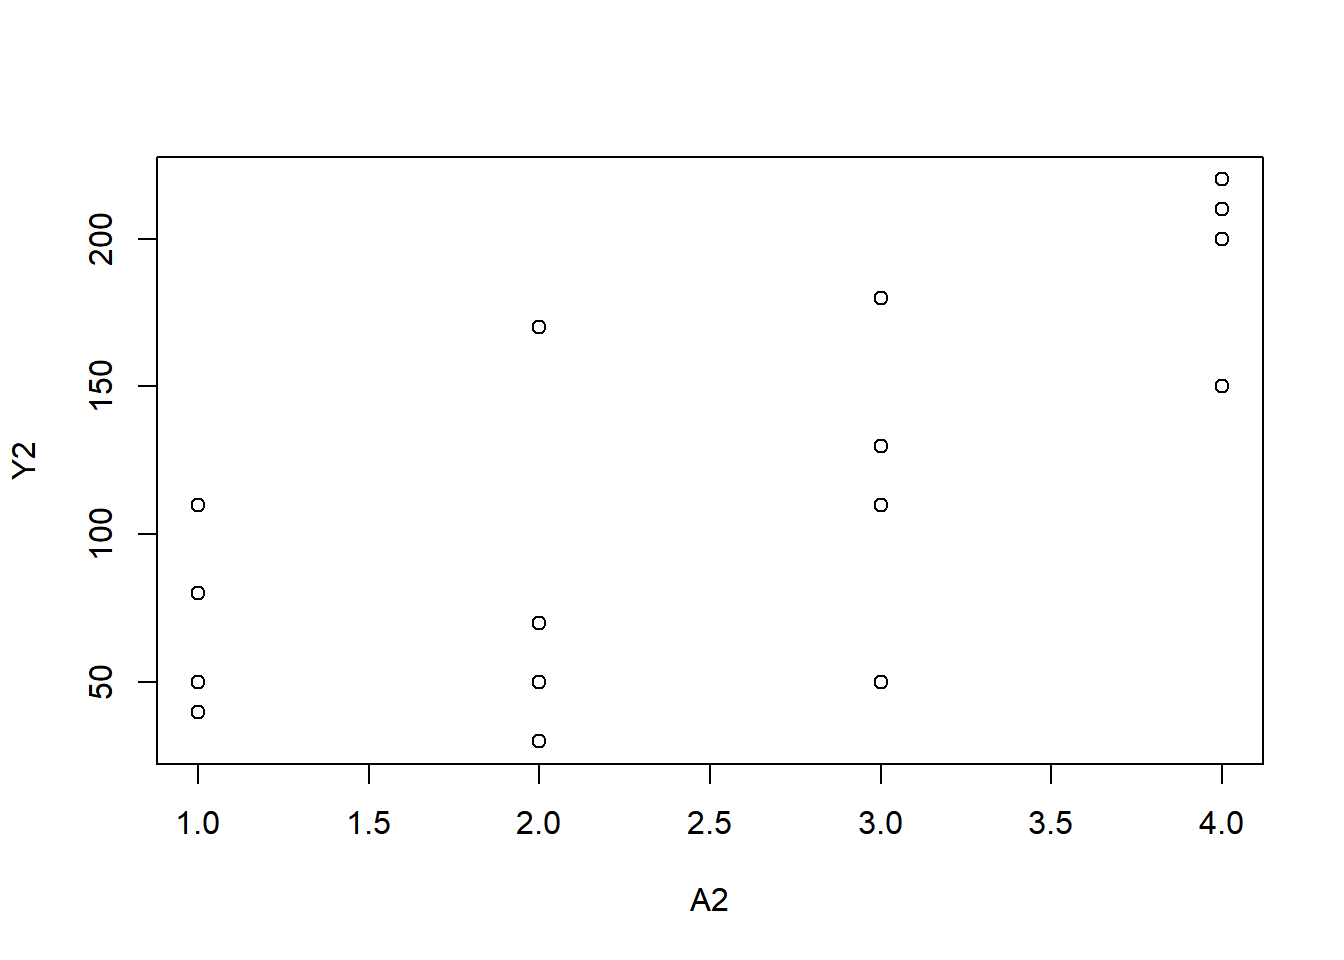
\includegraphics[width=0.85\linewidth]{15-prop-scores-r_files/figure-latex/unnamed-chunk-3-2} \end{center}

\begin{Shaded}
\begin{Highlighting}[]
\CommentTok{# attempt to reproduce plot from the book}
\NormalTok{nhefs }\OperatorTok
\StringTok{  }\KeywordTok{mutate}\NormalTok{(}\DataTypeTok{ps.grp =} \KeywordTok{round}\NormalTok{(ps}\OperatorTok{/}\FloatTok{0.05}\NormalTok{) }\OperatorTok{*}\StringTok{ }\FloatTok{0.05}\NormalTok{) }\OperatorTok
\StringTok{  }\KeywordTok{group_by}\NormalTok{(qsmk, ps.grp) }\OperatorTok
\StringTok{  }\KeywordTok{summarize}\NormalTok{(}\DataTypeTok{n =} \KeywordTok{n}\NormalTok{()) }\OperatorTok
\StringTok{  }\KeywordTok{ungroup}\NormalTok{() }\OperatorTok
\StringTok{  }\KeywordTok{mutate}\NormalTok{(}\DataTypeTok{n2 =} \KeywordTok{ifelse}\NormalTok{(qsmk }\OperatorTok{==}\StringTok{ }\DecValTok{0}\NormalTok{, }\DataTypeTok{yes =}\NormalTok{ n, }\DataTypeTok{no =}  \DecValTok{-1}\OperatorTok{*}\NormalTok{n)) }\OperatorTok
\StringTok{  }\KeywordTok{ggplot}\NormalTok{(}\KeywordTok{aes}\NormalTok{(}\DataTypeTok{x =}\NormalTok{ ps.grp, }\DataTypeTok{y =}\NormalTok{ n2, }\DataTypeTok{fill =} \KeywordTok{as.factor}\NormalTok{(qsmk))) }\OperatorTok{+}
\StringTok{  }\KeywordTok{geom_bar}\NormalTok{(}\DataTypeTok{stat =} \StringTok{'identity'}\NormalTok{, }\DataTypeTok{position =} \StringTok{'identity'}\NormalTok{) }\OperatorTok{+}
\StringTok{  }\KeywordTok{geom_text}\NormalTok{(}\KeywordTok{aes}\NormalTok{(}\DataTypeTok{label =}\NormalTok{ n, }\DataTypeTok{x =}\NormalTok{ ps.grp, }\DataTypeTok{y =}\NormalTok{ n2 }\OperatorTok{+}\StringTok{ }\KeywordTok{ifelse}\NormalTok{(qsmk }\OperatorTok{==}\StringTok{ }\DecValTok{0}\NormalTok{, }\DecValTok{8}\NormalTok{, }\DecValTok{-8}\NormalTok{))) }\OperatorTok{+}
\StringTok{  }\KeywordTok{xlab}\NormalTok{(}\StringTok{'Probability of Quitting Smoking During Follow-up'}\NormalTok{) }\OperatorTok{+}
\StringTok{  }\KeywordTok{ylab}\NormalTok{(}\StringTok{'N'}\NormalTok{) }\OperatorTok{+}
\StringTok{  }\KeywordTok{ggtitle}\NormalTok{(}\StringTok{'Propensity Score Distribution by Treatment Group'}\NormalTok{) }\OperatorTok{+}
\StringTok{  }\KeywordTok{scale_fill_discrete}\NormalTok{(}\StringTok{''}\NormalTok{) }\OperatorTok{+}
\StringTok{  }\KeywordTok{scale_x_continuous}\NormalTok{(}\DataTypeTok{breaks =} \KeywordTok{seq}\NormalTok{(}\DecValTok{0}\NormalTok{, }\DecValTok{1}\NormalTok{, }\FloatTok{0.05}\NormalTok{)) }\OperatorTok{+}
\StringTok{  }\KeywordTok{theme}\NormalTok{(}\DataTypeTok{legend.position =} \StringTok{'bottom'}\NormalTok{, }\DataTypeTok{legend.direction =} \StringTok{'vertical'}\NormalTok{,}
        \DataTypeTok{axis.ticks.y =} \KeywordTok{element_blank}\NormalTok{(),}
        \DataTypeTok{axis.text.y =} \KeywordTok{element_blank}\NormalTok{())}
\end{Highlighting}
\end{Shaded}

\hypertarget{program-15.3}{%
\section{Program 15.3}\label{program-15.3}}

\begin{itemize}
\tightlist
\item
  Stratification on the propensity score
\item
  Data from NHEFS
\end{itemize}

\begin{Shaded}
\begin{Highlighting}[]
\CommentTok{# calculation of deciles}
\NormalTok{nhefs}\OperatorTok{$}\NormalTok{ps.dec <-}\StringTok{ }\KeywordTok{cut}\NormalTok{(nhefs}\OperatorTok{$}\NormalTok{ps, }
                    \DataTypeTok{breaks=}\KeywordTok{c}\NormalTok{(}\KeywordTok{quantile}\NormalTok{(nhefs}\OperatorTok{$}\NormalTok{ps, }\DataTypeTok{probs=}\KeywordTok{seq}\NormalTok{(}\DecValTok{0}\NormalTok{,}\DecValTok{1}\NormalTok{,}\FloatTok{0.1}\NormalTok{))),}
                    \DataTypeTok{labels=}\KeywordTok{seq}\NormalTok{(}\DecValTok{1}\OperatorTok{:}\DecValTok{10}\NormalTok{),}
                    \DataTypeTok{include.lowest=}\OtherTok{TRUE}\NormalTok{)}

\CommentTok{#install.packages("psych") # install package if required}
\KeywordTok{library}\NormalTok{(}\StringTok{"psych"}\NormalTok{)}
\end{Highlighting}
\end{Shaded}

\begin{verbatim}
## 
## Attaching package: 'psych'
\end{verbatim}

\begin{verbatim}
## The following objects are masked from 'package:ggplot2':
## 
##     %+%, alpha
\end{verbatim}

\begin{Shaded}
\begin{Highlighting}[]
\KeywordTok{describeBy}\NormalTok{(nhefs}\OperatorTok{$}\NormalTok{ps, }\KeywordTok{list}\NormalTok{(nhefs}\OperatorTok{$}\NormalTok{ps.dec, nhefs}\OperatorTok{$}\NormalTok{qsmk))}
\end{Highlighting}
\end{Shaded}

\begin{verbatim}
## 
##  Descriptive statistics by group 
## : 1
## : 0
##    vars   n mean   sd median trimmed  mad  min  max range  skew kurtosis
## X1    1 151  0.1 0.02   0.11     0.1 0.02 0.05 0.13  0.08 -0.55    -0.53
##    se
## X1  0
## -------------------------------------------------------- 
## : 2
## : 0
##    vars   n mean   sd median trimmed  mad  min  max range  skew kurtosis
## X1    1 136 0.15 0.01   0.15    0.15 0.01 0.13 0.17  0.04 -0.04    -1.23
##    se
## X1  0
## -------------------------------------------------------- 
## : 3
## : 0
##    vars   n mean   sd median trimmed  mad  min  max range  skew kurtosis
## X1    1 134 0.18 0.01   0.18    0.18 0.01 0.17 0.19  0.03 -0.08    -1.34
##    se
## X1  0
## -------------------------------------------------------- 
## : 4
## : 0
##    vars   n mean   sd median trimmed  mad  min  max range  skew kurtosis
## X1    1 129 0.21 0.01   0.21    0.21 0.01 0.19 0.22  0.02 -0.04    -1.13
##    se
## X1  0
## -------------------------------------------------------- 
## : 5
## : 0
##    vars   n mean   sd median trimmed  mad  min  max range skew kurtosis se
## X1    1 120 0.23 0.01   0.23    0.23 0.01 0.22 0.25  0.03 0.24    -1.22  0
## -------------------------------------------------------- 
## : 6
## : 0
##    vars   n mean   sd median trimmed  mad  min  max range  skew kurtosis
## X1    1 117 0.26 0.01   0.26    0.26 0.01 0.25 0.27  0.03 -0.11    -1.29
##    se
## X1  0
## -------------------------------------------------------- 
## : 7
## : 0
##    vars   n mean   sd median trimmed  mad  min  max range  skew kurtosis
## X1    1 120 0.29 0.01   0.29    0.29 0.01 0.27 0.31  0.03 -0.23    -1.19
##    se
## X1  0
## -------------------------------------------------------- 
## : 8
## : 0
##    vars   n mean   sd median trimmed  mad  min  max range skew kurtosis se
## X1    1 112 0.33 0.01   0.33    0.33 0.02 0.31 0.35  0.04 0.15     -1.1  0
## -------------------------------------------------------- 
## : 9
## : 0
##    vars  n mean   sd median trimmed  mad  min  max range skew kurtosis se
## X1    1 96 0.38 0.02   0.38    0.38 0.02 0.35 0.42  0.06 0.13    -1.15  0
## -------------------------------------------------------- 
## : 10
## : 0
##    vars  n mean   sd median trimmed  mad  min  max range skew kurtosis
## X1    1 86 0.49 0.06   0.47    0.48 0.05 0.42 0.66  0.24  1.1     0.47
##      se
## X1 0.01
## -------------------------------------------------------- 
## : 1
## : 1
##    vars  n mean   sd median trimmed  mad  min  max range skew kurtosis
## X1    1 12  0.1 0.02   0.11     0.1 0.03 0.06 0.13  0.07 -0.5    -1.36
##      se
## X1 0.01
## -------------------------------------------------------- 
## : 2
## : 1
##    vars  n mean   sd median trimmed  mad  min  max range  skew kurtosis se
## X1    1 27 0.15 0.01   0.15    0.15 0.01 0.13 0.17  0.03 -0.03    -1.34  0
## -------------------------------------------------------- 
## : 3
## : 1
##    vars  n mean   sd median trimmed  mad  min  max range skew kurtosis se
## X1    1 29 0.18 0.01   0.18    0.18 0.01 0.17 0.19  0.03 0.01    -1.34  0
## -------------------------------------------------------- 
## : 4
## : 1
##    vars  n mean   sd median trimmed  mad  min  max range  skew kurtosis se
## X1    1 34 0.21 0.01   0.21    0.21 0.01 0.19 0.22  0.02 -0.31    -1.23  0
## -------------------------------------------------------- 
## : 5
## : 1
##    vars  n mean   sd median trimmed  mad  min  max range skew kurtosis se
## X1    1 43 0.23 0.01   0.23    0.23 0.01 0.22 0.25  0.03 0.11    -1.23  0
## -------------------------------------------------------- 
## : 6
## : 1
##    vars  n mean   sd median trimmed  mad  min  max range skew kurtosis se
## X1    1 45 0.26 0.01   0.26    0.26 0.01 0.25 0.27  0.03  0.2    -1.12  0
## -------------------------------------------------------- 
## : 7
## : 1
##    vars  n mean   sd median trimmed  mad  min  max range skew kurtosis se
## X1    1 43 0.29 0.01   0.29    0.29 0.01 0.27 0.31  0.03 0.16    -1.25  0
## -------------------------------------------------------- 
## : 8
## : 1
##    vars  n mean   sd median trimmed  mad  min  max range skew kurtosis se
## X1    1 51 0.33 0.01   0.33    0.33 0.02 0.31 0.35  0.04 0.11    -1.19  0
## -------------------------------------------------------- 
## : 9
## : 1
##    vars  n mean   sd median trimmed  mad  min  max range skew kurtosis se
## X1    1 67 0.38 0.02   0.38    0.38 0.03 0.35 0.42  0.06 0.19    -1.27  0
## -------------------------------------------------------- 
## : 10
## : 1
##    vars  n mean   sd median trimmed  mad  min  max range skew kurtosis
## X1    1 77 0.52 0.08   0.51    0.51 0.08 0.42 0.79  0.38 0.88     0.81
##      se
## X1 0.01
\end{verbatim}

\begin{Shaded}
\begin{Highlighting}[]
\CommentTok{# function to create deciles easily}
\NormalTok{decile <-}\StringTok{ }\ControlFlowTok{function}\NormalTok{(x) \{}
  \KeywordTok{return}\NormalTok{(}\KeywordTok{factor}\NormalTok{(}\KeywordTok{quantcut}\NormalTok{(x, }\KeywordTok{seq}\NormalTok{(}\DecValTok{0}\NormalTok{, }\DecValTok{1}\NormalTok{, }\FloatTok{0.1}\NormalTok{), }\DataTypeTok{labels =} \OtherTok{FALSE}\NormalTok{)))}
\NormalTok{\}}

\CommentTok{# regression on PS deciles, allowing for effect modification}
\ControlFlowTok{for}\NormalTok{ (deciles }\ControlFlowTok{in} \KeywordTok{c}\NormalTok{(}\DecValTok{1}\OperatorTok{:}\DecValTok{10}\NormalTok{)) \{}
  \KeywordTok{print}\NormalTok{(}\KeywordTok{t.test}\NormalTok{(wt82_}\DecValTok{71}\OperatorTok{~}\NormalTok{qsmk, }\DataTypeTok{data=}\NormalTok{nhefs[}\KeywordTok{which}\NormalTok{(nhefs}\OperatorTok{$}\NormalTok{ps.dec}\OperatorTok{==}\NormalTok{deciles),]))}
\NormalTok{\}}
\end{Highlighting}
\end{Shaded}

\begin{verbatim}
## 
##  Welch Two Sample t-test
## 
## data:  wt82_71 by qsmk
## t = 0.0060506, df = 11.571, p-value = 0.9953
## alternative hypothesis: true difference in means is not equal to 0
## 95 percent confidence interval:
##  -5.283903  5.313210
## sample estimates:
## mean in group 0 mean in group 1 
##        3.995205        3.980551 
## 
## 
##  Welch Two Sample t-test
## 
## data:  wt82_71 by qsmk
## t = -3.1117, df = 37.365, p-value = 0.003556
## alternative hypothesis: true difference in means is not equal to 0
## 95 percent confidence interval:
##  -6.849335 -1.448161
## sample estimates:
## mean in group 0 mean in group 1 
##        2.904679        7.053426 
## 
## 
##  Welch Two Sample t-test
## 
## data:  wt82_71 by qsmk
## t = -4.5301, df = 35.79, p-value = 6.317e-05
## alternative hypothesis: true difference in means is not equal to 0
## 95 percent confidence interval:
##  -9.474961 -3.613990
## sample estimates:
## mean in group 0 mean in group 1 
##        2.612094        9.156570 
## 
## 
##  Welch Two Sample t-test
## 
## data:  wt82_71 by qsmk
## t = -1.4117, df = 45.444, p-value = 0.1648
## alternative hypothesis: true difference in means is not equal to 0
## 95 percent confidence interval:
##  -5.6831731  0.9985715
## sample estimates:
## mean in group 0 mean in group 1 
##        3.474679        5.816979 
## 
## 
##  Welch Two Sample t-test
## 
## data:  wt82_71 by qsmk
## t = -3.1371, df = 74.249, p-value = 0.002446
## alternative hypothesis: true difference in means is not equal to 0
## 95 percent confidence interval:
##  -6.753621 -1.507087
## sample estimates:
## mean in group 0 mean in group 1 
##        2.098800        6.229154 
## 
## 
##  Welch Two Sample t-test
## 
## data:  wt82_71 by qsmk
## t = -2.1677, df = 50.665, p-value = 0.0349
## alternative hypothesis: true difference in means is not equal to 0
## 95 percent confidence interval:
##  -8.7516605 -0.3350127
## sample estimates:
## mean in group 0 mean in group 1 
##        1.847004        6.390340 
## 
## 
##  Welch Two Sample t-test
## 
## data:  wt82_71 by qsmk
## t = -3.3155, df = 84.724, p-value = 0.001348
## alternative hypothesis: true difference in means is not equal to 0
## 95 percent confidence interval:
##  -6.904207 -1.727590
## sample estimates:
## mean in group 0 mean in group 1 
##        1.560048        5.875946 
## 
## 
##  Welch Two Sample t-test
## 
## data:  wt82_71 by qsmk
## t = -2.664, df = 75.306, p-value = 0.009441
## alternative hypothesis: true difference in means is not equal to 0
## 95 percent confidence interval:
##  -6.2396014 -0.9005605
## sample estimates:
## mean in group 0 mean in group 1 
##       0.2846851       3.8547661 
## 
## 
##  Welch Two Sample t-test
## 
## data:  wt82_71 by qsmk
## t = -1.9122, df = 129.12, p-value = 0.05806
## alternative hypothesis: true difference in means is not equal to 0
## 95 percent confidence interval:
##  -4.68143608  0.07973698
## sample estimates:
## mean in group 0 mean in group 1 
##      -0.8954482       1.4054014 
## 
## 
##  Welch Two Sample t-test
## 
## data:  wt82_71 by qsmk
## t = -1.5925, df = 142.72, p-value = 0.1135
## alternative hypothesis: true difference in means is not equal to 0
## 95 percent confidence interval:
##  -5.0209284  0.5404697
## sample estimates:
## mean in group 0 mean in group 1 
##      -0.5043766       1.7358528
\end{verbatim}

\begin{Shaded}
\begin{Highlighting}[]
\CommentTok{# regression on PS deciles, not allowing for effect modification}
\NormalTok{fit.psdec <-}\StringTok{ }\KeywordTok{glm}\NormalTok{(wt82_}\DecValTok{71} \OperatorTok{~}\StringTok{ }\NormalTok{qsmk }\OperatorTok{+}\StringTok{ }\KeywordTok{as.factor}\NormalTok{(ps.dec), }\DataTypeTok{data =}\NormalTok{ nhefs)}
\KeywordTok{summary}\NormalTok{(fit.psdec)}
\end{Highlighting}
\end{Shaded}

\begin{verbatim}
## 
## Call:
## glm(formula = wt82_71 ~ qsmk + as.factor(ps.dec), data = nhefs)
## 
## Deviance Residuals: 
##     Min       1Q   Median       3Q      Max  
## -43.543   -3.932   -0.085    4.233   46.773  
## 
## Coefficients:
##                     Estimate Std. Error t value Pr(>|t|)    
## (Intercept)           3.7505     0.6089   6.159 9.29e-10 ***
## qsmk                  3.5005     0.4571   7.659 3.28e-14 ***
## as.factor(ps.dec)2   -0.7391     0.8611  -0.858   0.3908    
## as.factor(ps.dec)3   -0.6182     0.8612  -0.718   0.4730    
## as.factor(ps.dec)4   -0.5204     0.8584  -0.606   0.5444    
## as.factor(ps.dec)5   -1.4884     0.8590  -1.733   0.0834 .  
## as.factor(ps.dec)6   -1.6227     0.8675  -1.871   0.0616 .  
## as.factor(ps.dec)7   -1.9853     0.8681  -2.287   0.0223 *  
## as.factor(ps.dec)8   -3.4447     0.8749  -3.937 8.61e-05 ***
## as.factor(ps.dec)9   -5.1544     0.8848  -5.825 6.91e-09 ***
## as.factor(ps.dec)10  -4.8403     0.8828  -5.483 4.87e-08 ***
## ---
## Signif. codes:  0 '***' 0.001 '**' 0.01 '*' 0.05 '.' 0.1 ' ' 1
## 
## (Dispersion parameter for gaussian family taken to be 58.42297)
## 
##     Null deviance: 97176  on 1565  degrees of freedom
## Residual deviance: 90848  on 1555  degrees of freedom
##   (63 observations deleted due to missingness)
## AIC: 10827
## 
## Number of Fisher Scoring iterations: 2
\end{verbatim}

\begin{Shaded}
\begin{Highlighting}[]
\KeywordTok{confint.lm}\NormalTok{(fit.psdec)}
\end{Highlighting}
\end{Shaded}

\begin{verbatim}
##                         2.5 %      97.5 %
## (Intercept)          2.556098  4.94486263
## qsmk                 2.603953  4.39700504
## as.factor(ps.dec)2  -2.428074  0.94982494
## as.factor(ps.dec)3  -2.307454  1.07103569
## as.factor(ps.dec)4  -2.204103  1.16333143
## as.factor(ps.dec)5  -3.173337  0.19657938
## as.factor(ps.dec)6  -3.324345  0.07893027
## as.factor(ps.dec)7  -3.688043 -0.28248110
## as.factor(ps.dec)8  -5.160862 -1.72860113
## as.factor(ps.dec)9  -6.889923 -3.41883853
## as.factor(ps.dec)10 -6.571789 -3.10873731
\end{verbatim}

\hypertarget{program-15.4}{%
\section{Program 15.4}\label{program-15.4}}

\begin{itemize}
\tightlist
\item
  Standardization using the propensity score
\item
  Data from NHEFS
\end{itemize}

\begin{Shaded}
\begin{Highlighting}[]
\CommentTok{#install.packages("boot") # install package if required}
\KeywordTok{library}\NormalTok{(}\StringTok{"boot"}\NormalTok{)}
\end{Highlighting}
\end{Shaded}

\begin{verbatim}
## 
## Attaching package: 'boot'
\end{verbatim}

\begin{verbatim}
## The following object is masked from 'package:psych':
## 
##     logit
\end{verbatim}

\begin{verbatim}
## The following object is masked from 'package:survival':
## 
##     aml
\end{verbatim}

\begin{Shaded}
\begin{Highlighting}[]
\CommentTok{# standardization by propensity score, agnostic regarding effect modification }
\NormalTok{std.ps <-}\StringTok{ }\ControlFlowTok{function}\NormalTok{(data, indices) \{}
\NormalTok{  d <-}\StringTok{ }\NormalTok{data[indices,] }\CommentTok{# 1st copy: equal to original one`}
  \CommentTok{# calculating propensity scores}
\NormalTok{  ps.fit <-}\StringTok{ }\KeywordTok{glm}\NormalTok{(qsmk }\OperatorTok{~}\StringTok{ }\NormalTok{sex }\OperatorTok{+}\StringTok{ }\NormalTok{race }\OperatorTok{+}\StringTok{ }\NormalTok{age }\OperatorTok{+}\StringTok{ }\KeywordTok{I}\NormalTok{(age}\OperatorTok{*}\NormalTok{age) }
                \OperatorTok{+}\StringTok{ }\KeywordTok{as.factor}\NormalTok{(education) }\OperatorTok{+}\StringTok{ }\NormalTok{smokeintensity}
                \OperatorTok{+}\StringTok{ }\KeywordTok{I}\NormalTok{(smokeintensity}\OperatorTok{*}\NormalTok{smokeintensity) }\OperatorTok{+}\StringTok{ }\NormalTok{smokeyrs}
                \OperatorTok{+}\StringTok{ }\KeywordTok{I}\NormalTok{(smokeyrs}\OperatorTok{*}\NormalTok{smokeyrs) }\OperatorTok{+}\StringTok{ }\KeywordTok{as.factor}\NormalTok{(exercise)}
                \OperatorTok{+}\StringTok{ }\KeywordTok{as.factor}\NormalTok{(active) }\OperatorTok{+}\StringTok{ }\NormalTok{wt71 }\OperatorTok{+}\StringTok{ }\KeywordTok{I}\NormalTok{(wt71}\OperatorTok{*}\NormalTok{wt71),}
                \DataTypeTok{data=}\NormalTok{d, }\DataTypeTok{family=}\KeywordTok{binomial}\NormalTok{())}
\NormalTok{  d}\OperatorTok{$}\NormalTok{pscore <-}\StringTok{ }\KeywordTok{predict}\NormalTok{(ps.fit, d, }\DataTypeTok{type=}\StringTok{"response"}\NormalTok{)}
  
  \CommentTok{# create a dataset with 3 copies of each subject}
\NormalTok{  d}\OperatorTok{$}\NormalTok{interv <-}\StringTok{ }\DecValTok{-1} \CommentTok{# 1st copy: equal to original one`}
\NormalTok{  d0 <-}\StringTok{ }\NormalTok{d }\CommentTok{# 2nd copy: treatment set to 0, outcome to missing}
\NormalTok{  d0}\OperatorTok{$}\NormalTok{interv <-}\StringTok{ }\DecValTok{0}
\NormalTok{  d0}\OperatorTok{$}\NormalTok{qsmk <-}\StringTok{ }\DecValTok{0}
\NormalTok{  d0}\OperatorTok{$}\NormalTok{wt82_}\DecValTok{71}\NormalTok{ <-}\StringTok{ }\OtherTok{NA}
\NormalTok{  d1 <-}\StringTok{ }\NormalTok{d }\CommentTok{# 3rd copy: treatment set to 1, outcome to missing}
\NormalTok{  d1}\OperatorTok{$}\NormalTok{interv <-}\StringTok{ }\DecValTok{1}
\NormalTok{  d1}\OperatorTok{$}\NormalTok{qsmk <-}\StringTok{ }\DecValTok{1}
\NormalTok{  d1}\OperatorTok{$}\NormalTok{wt82_}\DecValTok{71}\NormalTok{ <-}\StringTok{ }\OtherTok{NA}
\NormalTok{  d.onesample <-}\StringTok{ }\KeywordTok{rbind}\NormalTok{(d, d0, d1) }\CommentTok{# combining datasets}

\NormalTok{  std.fit <-}\StringTok{ }\KeywordTok{glm}\NormalTok{(wt82_}\DecValTok{71} \OperatorTok{~}\StringTok{ }\NormalTok{qsmk }\OperatorTok{+}\StringTok{ }\NormalTok{pscore }\OperatorTok{+}\StringTok{ }\KeywordTok{I}\NormalTok{(qsmk}\OperatorTok{*}\NormalTok{pscore), }\DataTypeTok{data=}\NormalTok{d.onesample)}
\NormalTok{  d.onesample}\OperatorTok{$}\NormalTok{predicted_meanY <-}\StringTok{ }\KeywordTok{predict}\NormalTok{(std.fit, d.onesample)}

  \CommentTok{# estimate mean outcome in each of the groups interv=-1, interv=0, and interv=1}
  \KeywordTok{return}\NormalTok{(}\KeywordTok{c}\NormalTok{(}\KeywordTok{mean}\NormalTok{(d.onesample}\OperatorTok{$}\NormalTok{predicted_meanY[d.onesample}\OperatorTok{$}\NormalTok{interv}\OperatorTok{==-}\DecValTok{1}\NormalTok{]),}
           \KeywordTok{mean}\NormalTok{(d.onesample}\OperatorTok{$}\NormalTok{predicted_meanY[d.onesample}\OperatorTok{$}\NormalTok{interv}\OperatorTok{==}\DecValTok{0}\NormalTok{]),}
           \KeywordTok{mean}\NormalTok{(d.onesample}\OperatorTok{$}\NormalTok{predicted_meanY[d.onesample}\OperatorTok{$}\NormalTok{interv}\OperatorTok{==}\DecValTok{1}\NormalTok{]),}
           \KeywordTok{mean}\NormalTok{(d.onesample}\OperatorTok{$}\NormalTok{predicted_meanY[d.onesample}\OperatorTok{$}\NormalTok{interv}\OperatorTok{==}\DecValTok{1}\NormalTok{])}\OperatorTok{-}
\StringTok{             }\KeywordTok{mean}\NormalTok{(d.onesample}\OperatorTok{$}\NormalTok{predicted_meanY[d.onesample}\OperatorTok{$}\NormalTok{interv}\OperatorTok{==}\DecValTok{0}\NormalTok{])))}
\NormalTok{\}}

\CommentTok{# bootstrap}
\NormalTok{results <-}\StringTok{ }\KeywordTok{boot}\NormalTok{(}\DataTypeTok{data=}\NormalTok{nhefs, }\DataTypeTok{statistic=}\NormalTok{std.ps, }\DataTypeTok{R=}\DecValTok{5}\NormalTok{)}

\CommentTok{# generating confidence intervals}
\NormalTok{se <-}\StringTok{ }\KeywordTok{c}\NormalTok{(}\KeywordTok{sd}\NormalTok{(results}\OperatorTok{$}\NormalTok{t[,}\DecValTok{1}\NormalTok{]), }\KeywordTok{sd}\NormalTok{(results}\OperatorTok{$}\NormalTok{t[,}\DecValTok{2}\NormalTok{]), }
        \KeywordTok{sd}\NormalTok{(results}\OperatorTok{$}\NormalTok{t[,}\DecValTok{3}\NormalTok{]), }\KeywordTok{sd}\NormalTok{(results}\OperatorTok{$}\NormalTok{t[,}\DecValTok{4}\NormalTok{]))}
\NormalTok{mean <-}\StringTok{ }\NormalTok{results}\OperatorTok{$}\NormalTok{t0}
\NormalTok{ll <-}\StringTok{ }\NormalTok{mean }\OperatorTok{-}\StringTok{ }\KeywordTok{qnorm}\NormalTok{(}\FloatTok{0.975}\NormalTok{)}\OperatorTok{*}\NormalTok{se}
\NormalTok{ul <-}\StringTok{ }\NormalTok{mean }\OperatorTok{+}\StringTok{ }\KeywordTok{qnorm}\NormalTok{(}\FloatTok{0.975}\NormalTok{)}\OperatorTok{*}\NormalTok{se}

\NormalTok{bootstrap <-}\StringTok{ }\KeywordTok{data.frame}\NormalTok{(}\KeywordTok{cbind}\NormalTok{(}\KeywordTok{c}\NormalTok{(}\StringTok{"Observed"}\NormalTok{, }\StringTok{"No Treatment"}\NormalTok{, }\StringTok{"Treatment"}\NormalTok{, }
                                \StringTok{"Treatment - No Treatment"}\NormalTok{), mean, se, ll, ul))}
\NormalTok{bootstrap}
\end{Highlighting}
\end{Shaded}

\begin{verbatim}
##                         V1             mean                se
## 1                 Observed 2.63384609228479 0.211907881812535
## 2             No Treatment 1.71983636149843 0.407033276190538
## 3                Treatment 5.35072300362993 0.329039146109479
## 4 Treatment - No Treatment 3.63088664213151 0.639564046239437
##                  ll               ul
## 1  2.21851427589206 3.04917790867753
## 2 0.922065799655627 2.51760692334122
## 3  4.70581812775154 5.99562787950832
## 4   2.3773641456955 4.88440913856751
\end{verbatim}

\begin{Shaded}
\begin{Highlighting}[]
\CommentTok{# regression on the propensity score (linear term)}
\NormalTok{model6 <-}\StringTok{ }\KeywordTok{glm}\NormalTok{(wt82_}\DecValTok{71} \OperatorTok{~}\StringTok{ }\NormalTok{qsmk }\OperatorTok{+}\StringTok{ }\NormalTok{ps, }\DataTypeTok{data =}\NormalTok{ nhefs) }\CommentTok{# p.qsmk}
\KeywordTok{summary}\NormalTok{(model6)}
\end{Highlighting}
\end{Shaded}

\begin{verbatim}
## 
## Call:
## glm(formula = wt82_71 ~ qsmk + ps, data = nhefs)
## 
## Deviance Residuals: 
##     Min       1Q   Median       3Q      Max  
## -43.314   -4.006   -0.068    4.244   47.158  
## 
## Coefficients:
##             Estimate Std. Error t value Pr(>|t|)    
## (Intercept)   5.5945     0.4831  11.581  < 2e-16 ***
## qsmk          3.5506     0.4573   7.765 1.47e-14 ***
## ps          -14.8218     1.7576  -8.433  < 2e-16 ***
## ---
## Signif. codes:  0 '***' 0.001 '**' 0.01 '*' 0.05 '.' 0.1 ' ' 1
## 
## (Dispersion parameter for gaussian family taken to be 58.28455)
## 
##     Null deviance: 97176  on 1565  degrees of freedom
## Residual deviance: 91099  on 1563  degrees of freedom
##   (63 observations deleted due to missingness)
## AIC: 10815
## 
## Number of Fisher Scoring iterations: 2
\end{verbatim}

\begin{Shaded}
\begin{Highlighting}[]
\CommentTok{# standarization on the propensity score}
\CommentTok{# (step 1) create two new datasets, one with all treated and one with all untreated}
\NormalTok{treated <-}\StringTok{ }\NormalTok{nhefs}
\NormalTok{  treated}\OperatorTok{$}\NormalTok{qsmk <-}\StringTok{ }\DecValTok{1}

\NormalTok{untreated <-}\StringTok{ }\NormalTok{nhefs}
\NormalTok{  untreated}\OperatorTok{$}\NormalTok{qsmk <-}\StringTok{ }\DecValTok{0}

\CommentTok{# (step 2) predict values for everyone in each new dataset based on above model}
\NormalTok{treated}\OperatorTok{$}\NormalTok{pred.y <-}\StringTok{ }\KeywordTok{predict}\NormalTok{(model6, treated)}
\NormalTok{untreated}\OperatorTok{$}\NormalTok{pred.y <-}\StringTok{ }\KeywordTok{predict}\NormalTok{(model6, untreated)}

\CommentTok{# (step 3) compare mean weight loss had all been treated vs. that had all been untreated}
\NormalTok{mean1 <-}\StringTok{ }\KeywordTok{mean}\NormalTok{(treated}\OperatorTok{$}\NormalTok{pred.y, }\DataTypeTok{na.rm =} \OtherTok{TRUE}\NormalTok{)}
\NormalTok{mean0 <-}\StringTok{ }\KeywordTok{mean}\NormalTok{(untreated}\OperatorTok{$}\NormalTok{pred.y, }\DataTypeTok{na.rm =} \OtherTok{TRUE}\NormalTok{)}
\NormalTok{mean1}
\end{Highlighting}
\end{Shaded}

\begin{verbatim}
## [1] 5.250824
\end{verbatim}

\begin{Shaded}
\begin{Highlighting}[]
\NormalTok{mean0}
\end{Highlighting}
\end{Shaded}

\begin{verbatim}
## [1] 1.700228
\end{verbatim}

\begin{Shaded}
\begin{Highlighting}[]
\NormalTok{mean1 }\OperatorTok{-}\StringTok{ }\NormalTok{mean0}
\end{Highlighting}
\end{Shaded}

\begin{verbatim}
## [1] 3.550596
\end{verbatim}

\begin{Shaded}
\begin{Highlighting}[]
\CommentTok{# (step 4) bootstrap a confidence interval}
\CommentTok{# number of bootstraps}
\NormalTok{nboot <-}\StringTok{ }\DecValTok{100}
\CommentTok{# set up a matrix to store results}
\NormalTok{boots <-}\StringTok{ }\KeywordTok{data.frame}\NormalTok{(}\DataTypeTok{i =} \DecValTok{1}\OperatorTok{:}\NormalTok{nboot,}
                    \DataTypeTok{mean1 =} \OtherTok{NA}\NormalTok{,}
                    \DataTypeTok{mean0 =} \OtherTok{NA}\NormalTok{,}
                    \DataTypeTok{difference =} \OtherTok{NA}\NormalTok{)}
\CommentTok{# loop to perform the bootstrapping}
\NormalTok{nhefs <-}\StringTok{ }\KeywordTok{subset}\NormalTok{(nhefs, }\OperatorTok{!}\KeywordTok{is.na}\NormalTok{(ps) }\OperatorTok{&}\StringTok{ }\OperatorTok{!}\KeywordTok{is.na}\NormalTok{(wt82_}\DecValTok{71}\NormalTok{)) }\CommentTok{# p.qsmk}
\ControlFlowTok{for}\NormalTok{(i }\ControlFlowTok{in} \DecValTok{1}\OperatorTok{:}\NormalTok{nboot) \{}
  \CommentTok{# sample with replacement}
\NormalTok{  sampl <-}\StringTok{ }\NormalTok{nhefs[}\KeywordTok{sample}\NormalTok{(}\DecValTok{1}\OperatorTok{:}\KeywordTok{nrow}\NormalTok{(nhefs), }\KeywordTok{nrow}\NormalTok{(nhefs), }\DataTypeTok{replace =} \OtherTok{TRUE}\NormalTok{), ]}
  
  \CommentTok{# fit the model in the bootstrap sample}
\NormalTok{  bootmod <-}\StringTok{ }\KeywordTok{glm}\NormalTok{(wt82_}\DecValTok{71} \OperatorTok{~}\StringTok{ }\NormalTok{qsmk }\OperatorTok{+}\StringTok{ }\NormalTok{ps, }\DataTypeTok{data =}\NormalTok{ sampl) }\CommentTok{# ps}
  
  \CommentTok{# create new datasets}
\NormalTok{  sampl.treated <-}\StringTok{ }\NormalTok{sampl }\OperatorTok
\StringTok{    }\KeywordTok{mutate}\NormalTok{(}\DataTypeTok{qsmk =} \DecValTok{1}\NormalTok{)}
  
\NormalTok{  sampl.untreated <-}\StringTok{ }\NormalTok{sampl }\OperatorTok
\StringTok{    }\KeywordTok{mutate}\NormalTok{(}\DataTypeTok{qsmk =} \DecValTok{0}\NormalTok{)}
  
  \CommentTok{# predict values}
\NormalTok{  sampl.treated}\OperatorTok{$}\NormalTok{pred.y <-}\StringTok{ }\KeywordTok{predict}\NormalTok{(bootmod, sampl.treated)}
\NormalTok{  sampl.untreated}\OperatorTok{$}\NormalTok{pred.y <-}\StringTok{ }\KeywordTok{predict}\NormalTok{(bootmod, sampl.untreated)}
  
  \CommentTok{# output results }
\NormalTok{  boots[i, }\StringTok{'mean1'}\NormalTok{] <-}\StringTok{ }\KeywordTok{mean}\NormalTok{(sampl.treated}\OperatorTok{$}\NormalTok{pred.y, }\DataTypeTok{na.rm =} \OtherTok{TRUE}\NormalTok{)}
\NormalTok{  boots[i, }\StringTok{'mean0'}\NormalTok{] <-}\StringTok{ }\KeywordTok{mean}\NormalTok{(sampl.untreated}\OperatorTok{$}\NormalTok{pred.y, }\DataTypeTok{na.rm =} \OtherTok{TRUE}\NormalTok{)}
\NormalTok{  boots[i, }\StringTok{'difference'}\NormalTok{] <-}\StringTok{ }\NormalTok{boots[i, }\StringTok{'mean1'}\NormalTok{] }\OperatorTok{-}\StringTok{ }\NormalTok{boots[i, }\StringTok{'mean0'}\NormalTok{]}
  
  \CommentTok{# once loop is done, print the results}
  \ControlFlowTok{if}\NormalTok{(i }\OperatorTok{==}\StringTok{ }\NormalTok{nboot) \{}
    \KeywordTok{cat}\NormalTok{(}\StringTok{'95% CI for the causal mean difference}\CharTok{\textbackslash{}n}\StringTok{'}\NormalTok{)}
    \KeywordTok{cat}\NormalTok{(}\KeywordTok{mean}\NormalTok{(boots}\OperatorTok{$}\NormalTok{difference) }\OperatorTok{-}\StringTok{ }\FloatTok{1.96}\OperatorTok{*}\KeywordTok{sd}\NormalTok{(boots}\OperatorTok{$}\NormalTok{difference), }
        \StringTok{','}\NormalTok{,}
        \KeywordTok{mean}\NormalTok{(boots}\OperatorTok{$}\NormalTok{difference) }\OperatorTok{+}\StringTok{ }\FloatTok{1.96}\OperatorTok{*}\KeywordTok{sd}\NormalTok{(boots}\OperatorTok{$}\NormalTok{difference))}
\NormalTok{  \}}
\NormalTok{\}}
\end{Highlighting}
\end{Shaded}

\begin{verbatim}
## 95% CI for the causal mean difference
## 2.623614 , 4.656303
\end{verbatim}

A more flexible and elegant way to do this is to write a function to perform the model fitting, prediction, bootstrapping, and reporting all at once.

\hypertarget{instrumental-variables-estimation}{%
\chapter*{16. Instrumental variables estimation}\label{instrumental-variables-estimation}}
\addcontentsline{toc}{chapter}{16. Instrumental variables estimation}

\hypertarget{program-16.1}{%
\section{Program 16.1}\label{program-16.1}}

\begin{itemize}
\tightlist
\item
  Estimating the average causal using the standard IV estimator via the calculation of sample averages
\item
  Data from NHEFS
\end{itemize}

\begin{Shaded}
\begin{Highlighting}[]
\KeywordTok{library}\NormalTok{(here)}
\end{Highlighting}
\end{Shaded}

\begin{Shaded}
\begin{Highlighting}[]
\CommentTok{#install.packages("readxl") # install package if required}
\KeywordTok{library}\NormalTok{(}\StringTok{"readxl"}\NormalTok{)}
\NormalTok{nhefs <-}\StringTok{ }\KeywordTok{read_excel}\NormalTok{(}\KeywordTok{here}\NormalTok{(}\StringTok{"data"}\NormalTok{, }\StringTok{"NHEFS.xls"}\NormalTok{))}

\CommentTok{# some preprocessing of the data}
\NormalTok{nhefs}\OperatorTok{$}\NormalTok{cens <-}\StringTok{ }\KeywordTok{ifelse}\NormalTok{(}\KeywordTok{is.na}\NormalTok{(nhefs}\OperatorTok{$}\NormalTok{wt82), }\DecValTok{1}\NormalTok{, }\DecValTok{0}\NormalTok{)}
\KeywordTok{summary}\NormalTok{(nhefs}\OperatorTok{$}\NormalTok{price82)}
\end{Highlighting}
\end{Shaded}

\begin{verbatim}
##    Min. 1st Qu.  Median    Mean 3rd Qu.    Max.    NA's 
##   1.452   1.740   1.815   1.806   1.868   2.103      92
\end{verbatim}

\begin{Shaded}
\begin{Highlighting}[]
\CommentTok{# for simplicity, ignore subjects with missing outcome or missing instrument}
\NormalTok{nhefs.iv <-}\StringTok{ }\NormalTok{nhefs[}\KeywordTok{which}\NormalTok{(}\OperatorTok{!}\KeywordTok{is.na}\NormalTok{(nhefs}\OperatorTok{$}\NormalTok{wt82) }\OperatorTok{&}\StringTok{ }\OperatorTok{!}\KeywordTok{is.na}\NormalTok{(nhefs}\OperatorTok{$}\NormalTok{price82)),]}
\NormalTok{nhefs.iv}\OperatorTok{$}\NormalTok{highprice <-}\StringTok{ }\KeywordTok{ifelse}\NormalTok{(nhefs.iv}\OperatorTok{$}\NormalTok{price82}\OperatorTok{>=}\FloatTok{1.5}\NormalTok{, }\DecValTok{1}\NormalTok{, }\DecValTok{0}\NormalTok{)}

\KeywordTok{table}\NormalTok{(nhefs.iv}\OperatorTok{$}\NormalTok{highprice, nhefs.iv}\OperatorTok{$}\NormalTok{qsmk)}
\end{Highlighting}
\end{Shaded}

\begin{verbatim}
##    
##        0    1
##   0   33    8
##   1 1065  370
\end{verbatim}

\begin{Shaded}
\begin{Highlighting}[]
\KeywordTok{t.test}\NormalTok{(wt82_}\DecValTok{71} \OperatorTok{~}\StringTok{ }\NormalTok{highprice, }\DataTypeTok{data=}\NormalTok{nhefs.iv)}
\end{Highlighting}
\end{Shaded}

\begin{verbatim}
## 
##  Welch Two Sample t-test
## 
## data:  wt82_71 by highprice
## t = -0.10179, df = 41.644, p-value = 0.9194
## alternative hypothesis: true difference in means is not equal to 0
## 95 percent confidence interval:
##  -3.130588  2.830010
## sample estimates:
## mean in group 0 mean in group 1 
##        2.535729        2.686018
\end{verbatim}

\hypertarget{program-16.2}{%
\section{Program 16.2}\label{program-16.2}}

\begin{itemize}
\tightlist
\item
  Estimating the average causal effect using the standard IV estimator via two-stage-least-squares regression
\item
  Data from NHEFS
\end{itemize}

\begin{Shaded}
\begin{Highlighting}[]
\CommentTok{#install.packages ("sem") # install package if required}
\KeywordTok{library}\NormalTok{(sem) }

\NormalTok{model1 <-}\StringTok{ }\KeywordTok{tsls}\NormalTok{(wt82_}\DecValTok{71} \OperatorTok{~}\StringTok{ }\NormalTok{qsmk, }\OperatorTok{~}\StringTok{ }\NormalTok{highprice, }\DataTypeTok{data =}\NormalTok{ nhefs.iv)}
\KeywordTok{summary}\NormalTok{(model1)}
\end{Highlighting}
\end{Shaded}

\begin{verbatim}
## 
##  2SLS Estimates
## 
## Model Formula: wt82_71 ~ qsmk
## 
## Instruments: ~highprice
## 
## Residuals:
##      Min.   1st Qu.    Median      Mean   3rd Qu.      Max. 
## -43.34863  -4.00206  -0.02712   0.00000   4.17040  46.47022 
## 
##              Estimate Std. Error t value Pr(>|t|)
## (Intercept)  2.068164   5.085098 0.40671  0.68428
## qsmk         2.396270  19.840037 0.12078  0.90388
## 
## Residual standard error: 7.8561141 on 1474 degrees of freedom
\end{verbatim}

\begin{Shaded}
\begin{Highlighting}[]
\KeywordTok{confint}\NormalTok{(model1)  }\CommentTok{# note the wide confidence intervals}
\end{Highlighting}
\end{Shaded}

\begin{verbatim}
##                  2.5 %   97.5 %
## (Intercept)  -7.898445 12.03477
## qsmk        -36.489487 41.28203
\end{verbatim}

\hypertarget{program-16.3}{%
\section{Program 16.3}\label{program-16.3}}

\begin{itemize}
\tightlist
\item
  Estimating the average causal using the standard IV estimator via additive marginal structural models
\item
  Data from NHEFS
\item
  G-estimation: Checking one possible value of psi
\item
  See Chapter 14 for program that checks several values and computes 95\% confidence intervals
\end{itemize}

\begin{Shaded}
\begin{Highlighting}[]
\NormalTok{nhefs.iv}\OperatorTok{$}\NormalTok{psi <-}\StringTok{ }\FloatTok{2.396}
\NormalTok{nhefs.iv}\OperatorTok{$}\NormalTok{Hpsi <-}\StringTok{ }\NormalTok{nhefs.iv}\OperatorTok{$}\NormalTok{wt82_}\DecValTok{71}\OperatorTok{-}\NormalTok{nhefs.iv}\OperatorTok{$}\NormalTok{psi}\OperatorTok{*}\NormalTok{nhefs.iv}\OperatorTok{$}\NormalTok{qsmk}

\CommentTok{#install.packages("geepack") # install package if required}
\KeywordTok{library}\NormalTok{(}\StringTok{"geepack"}\NormalTok{)}
\NormalTok{g.est <-}\StringTok{ }\KeywordTok{geeglm}\NormalTok{(highprice }\OperatorTok{~}\StringTok{ }\NormalTok{Hpsi, }\DataTypeTok{data=}\NormalTok{nhefs.iv, }\DataTypeTok{id=}\NormalTok{seqn, }\DataTypeTok{family=}\KeywordTok{binomial}\NormalTok{(),}
                \DataTypeTok{corstr=}\StringTok{"independence"}\NormalTok{)}
\KeywordTok{summary}\NormalTok{(g.est)}
\end{Highlighting}
\end{Shaded}

\begin{verbatim}
## 
## Call:
## geeglm(formula = highprice ~ Hpsi, family = binomial(), data = nhefs.iv, 
##     id = seqn, corstr = "independence")
## 
##  Coefficients:
##              Estimate   Std.err  Wald Pr(>|W|)    
## (Intercept) 3.555e+00 1.652e-01 463.1   <2e-16 ***
## Hpsi        2.748e-07 2.273e-02   0.0        1    
## ---
## Signif. codes:  0 '***' 0.001 '**' 0.01 '*' 0.05 '.' 0.1 ' ' 1
## 
## Estimated Scale Parameters:
##             Estimate Std.err
## (Intercept)        1  0.7607
## 
## Correlation: Structure = independenceNumber of clusters:   1476   Maximum cluster size: 1
\end{verbatim}

\begin{Shaded}
\begin{Highlighting}[]
\NormalTok{beta <-}\StringTok{ }\KeywordTok{coef}\NormalTok{(g.est)}
\NormalTok{SE <-}\StringTok{ }\KeywordTok{coef}\NormalTok{(}\KeywordTok{summary}\NormalTok{(g.est))[,}\DecValTok{2}\NormalTok{]}
\NormalTok{lcl <-}\StringTok{ }\NormalTok{beta}\OperatorTok{-}\KeywordTok{qnorm}\NormalTok{(}\FloatTok{0.975}\NormalTok{)}\OperatorTok{*}\NormalTok{SE }
\NormalTok{ucl <-}\StringTok{ }\NormalTok{beta}\OperatorTok{+}\KeywordTok{qnorm}\NormalTok{(}\FloatTok{0.975}\NormalTok{)}\OperatorTok{*}\NormalTok{SE}
\KeywordTok{cbind}\NormalTok{(beta, lcl, ucl)}
\end{Highlighting}
\end{Shaded}

\begin{verbatim}
##                  beta      lcl     ucl
## (Intercept) 3.555e+00  3.23152 3.87917
## Hpsi        2.748e-07 -0.04456 0.04456
\end{verbatim}

\hypertarget{program-16.4}{%
\section{Program 16.4}\label{program-16.4}}

\begin{itemize}
\tightlist
\item
  Estimating the average causal using the standard IV estimator with altnerative proposed instruments
\item
  Data from NHEFS
\end{itemize}

\begin{Shaded}
\begin{Highlighting}[]
\KeywordTok{summary}\NormalTok{(}\KeywordTok{tsls}\NormalTok{(wt82_}\DecValTok{71} \OperatorTok{~}\StringTok{ }\NormalTok{qsmk, }\OperatorTok{~}\StringTok{ }\KeywordTok{ifelse}\NormalTok{(price82 }\OperatorTok{>=}\StringTok{ }\FloatTok{1.6}\NormalTok{, }\DecValTok{1}\NormalTok{, }\DecValTok{0}\NormalTok{), }\DataTypeTok{data =}\NormalTok{ nhefs.iv))}
\end{Highlighting}
\end{Shaded}

\begin{verbatim}
## 
##  2SLS Estimates
## 
## Model Formula: wt82_71 ~ qsmk
## 
## Instruments: ~ifelse(price82 >= 1.6, 1, 0)
## 
## Residuals:
##    Min. 1st Qu.  Median    Mean 3rd Qu.    Max. 
##   -55.6   -13.5     7.6     0.0    12.5    56.4 
## 
##             Estimate Std. Error t value Pr(>|t|)
## (Intercept)    -7.89      42.25  -0.187    0.852
## qsmk           41.28     164.95   0.250    0.802
## 
## Residual standard error: 18.6055 on 1474 degrees of freedom
\end{verbatim}

\begin{Shaded}
\begin{Highlighting}[]
\KeywordTok{summary}\NormalTok{(}\KeywordTok{tsls}\NormalTok{(wt82_}\DecValTok{71} \OperatorTok{~}\StringTok{ }\NormalTok{qsmk, }\OperatorTok{~}\StringTok{ }\KeywordTok{ifelse}\NormalTok{(price82 }\OperatorTok{>=}\StringTok{ }\FloatTok{1.7}\NormalTok{, }\DecValTok{1}\NormalTok{, }\DecValTok{0}\NormalTok{), }\DataTypeTok{data =}\NormalTok{ nhefs.iv))}
\end{Highlighting}
\end{Shaded}

\begin{verbatim}
## 
##  2SLS Estimates
## 
## Model Formula: wt82_71 ~ qsmk
## 
## Instruments: ~ifelse(price82 >= 1.7, 1, 0)
## 
## Residuals:
##    Min. 1st Qu.  Median    Mean 3rd Qu.    Max. 
##   -54.4   -13.4    -8.4     0.0    18.1    75.3 
## 
##             Estimate Std. Error t value Pr(>|t|)
## (Intercept)    13.16      48.08   0.274    0.784
## qsmk          -40.91     187.74  -0.218    0.828
## 
## Residual standard error: 20.591 on 1474 degrees of freedom
\end{verbatim}

\begin{Shaded}
\begin{Highlighting}[]
\KeywordTok{summary}\NormalTok{(}\KeywordTok{tsls}\NormalTok{(wt82_}\DecValTok{71} \OperatorTok{~}\StringTok{ }\NormalTok{qsmk, }\OperatorTok{~}\StringTok{ }\KeywordTok{ifelse}\NormalTok{(price82 }\OperatorTok{>=}\StringTok{ }\FloatTok{1.8}\NormalTok{, }\DecValTok{1}\NormalTok{, }\DecValTok{0}\NormalTok{), }\DataTypeTok{data =}\NormalTok{ nhefs.iv))}
\end{Highlighting}
\end{Shaded}

\begin{verbatim}
## 
##  2SLS Estimates
## 
## Model Formula: wt82_71 ~ qsmk
## 
## Instruments: ~ifelse(price82 >= 1.8, 1, 0)
## 
## Residuals:
##    Min. 1st Qu.  Median    Mean 3rd Qu.    Max. 
##  -49.37   -8.31   -3.44    0.00    7.27   60.53 
## 
##             Estimate Std. Error t value Pr(>|t|)
## (Intercept)    8.086      7.288   1.110    0.267
## qsmk         -21.103     28.428  -0.742    0.458
## 
## Residual standard error: 13.0188 on 1474 degrees of freedom
\end{verbatim}

\begin{Shaded}
\begin{Highlighting}[]
\KeywordTok{summary}\NormalTok{(}\KeywordTok{tsls}\NormalTok{(wt82_}\DecValTok{71} \OperatorTok{~}\StringTok{ }\NormalTok{qsmk, }\OperatorTok{~}\StringTok{ }\KeywordTok{ifelse}\NormalTok{(price82 }\OperatorTok{>=}\StringTok{ }\FloatTok{1.9}\NormalTok{, }\DecValTok{1}\NormalTok{, }\DecValTok{0}\NormalTok{), }\DataTypeTok{data =}\NormalTok{ nhefs.iv))}
\end{Highlighting}
\end{Shaded}

\begin{verbatim}
## 
##  2SLS Estimates
## 
## Model Formula: wt82_71 ~ qsmk
## 
## Instruments: ~ifelse(price82 >= 1.9, 1, 0)
## 
## Residuals:
##    Min. 1st Qu.  Median    Mean 3rd Qu.    Max. 
##  -47.24   -6.33   -1.43    0.00    5.52   54.36 
## 
##             Estimate Std. Error t value Pr(>|t|)
## (Intercept)    5.963      6.067   0.983    0.326
## qsmk         -12.811     23.667  -0.541    0.588
## 
## Residual standard error: 10.3637 on 1474 degrees of freedom
\end{verbatim}

\hypertarget{program-16.5}{%
\section{Program 16.5}\label{program-16.5}}

\begin{itemize}
\tightlist
\item
  Estimating the average causal using the standard IV estimator
\item
  Conditional on baseline covariates
\item
  Data from NHEFS
\end{itemize}

\begin{Shaded}
\begin{Highlighting}[]
\NormalTok{model2 <-}\StringTok{ }\KeywordTok{tsls}\NormalTok{(wt82_}\DecValTok{71} \OperatorTok{~}\StringTok{ }\NormalTok{qsmk }\OperatorTok{+}\StringTok{ }\NormalTok{sex }\OperatorTok{+}\StringTok{ }\NormalTok{race }\OperatorTok{+}\StringTok{ }\NormalTok{age }\OperatorTok{+}\StringTok{ }\NormalTok{smokeintensity }\OperatorTok{+}\StringTok{ }\NormalTok{smokeyrs }\OperatorTok{+}\StringTok{ }
\StringTok{                      }\KeywordTok{as.factor}\NormalTok{(exercise) }\OperatorTok{+}\StringTok{ }\KeywordTok{as.factor}\NormalTok{(active) }\OperatorTok{+}\StringTok{ }\NormalTok{wt71,}
             \OperatorTok{~}\StringTok{ }\NormalTok{highprice }\OperatorTok{+}\StringTok{ }\NormalTok{sex }\OperatorTok{+}\StringTok{ }\NormalTok{race }\OperatorTok{+}\StringTok{ }\NormalTok{age }\OperatorTok{+}\StringTok{ }\NormalTok{smokeintensity }\OperatorTok{+}\StringTok{ }\NormalTok{smokeyrs }\OperatorTok{+}\StringTok{ }\KeywordTok{as.factor}\NormalTok{(exercise) }\OperatorTok{+}
\StringTok{               }\KeywordTok{as.factor}\NormalTok{(active) }\OperatorTok{+}\StringTok{ }\NormalTok{wt71, }\DataTypeTok{data =}\NormalTok{ nhefs.iv)}
\KeywordTok{summary}\NormalTok{(model2)}
\end{Highlighting}
\end{Shaded}

\begin{verbatim}
## 
##  2SLS Estimates
## 
## Model Formula: wt82_71 ~ qsmk + sex + race + age + smokeintensity + smokeyrs + 
##     as.factor(exercise) + as.factor(active) + wt71
## 
## Instruments: ~highprice + sex + race + age + smokeintensity + smokeyrs + as.factor(exercise) + 
##     as.factor(active) + wt71
## 
## Residuals:
##    Min. 1st Qu.  Median    Mean 3rd Qu.    Max. 
##  -42.23   -4.29   -0.62    0.00    3.87   46.74 
## 
##                       Estimate Std. Error t value Pr(>|t|)    
## (Intercept)          17.280330   2.335402   7.399  2.3e-13 ***
## qsmk                 -1.042295  29.987369  -0.035   0.9723    
## sex                  -1.644393   2.630831  -0.625   0.5320    
## race                 -0.183255   4.650386  -0.039   0.9686    
## age                  -0.163640   0.240548  -0.680   0.4964    
## smokeintensity        0.005767   0.145504   0.040   0.9684    
## smokeyrs              0.025836   0.161421   0.160   0.8729    
## as.factor(exercise)1  0.498748   2.171239   0.230   0.8184    
## as.factor(exercise)2  0.581834   2.183148   0.267   0.7899    
## as.factor(active)1   -1.170145   0.607466  -1.926   0.0543 .  
## as.factor(active)2   -0.512284   1.308451  -0.392   0.6955    
## wt71                 -0.097949   0.036271  -2.701   0.0070 ** 
## ---
## Signif. codes:  0 '***' 0.001 '**' 0.01 '*' 0.05 '.' 0.1 ' ' 1
## 
## Residual standard error: 7.7162 on 1464 degrees of freedom
\end{verbatim}

\hypertarget{causal-survival-analysis}{%
\chapter*{17. Causal survival analysis}\label{causal-survival-analysis}}
\addcontentsline{toc}{chapter}{17. Causal survival analysis}

\hypertarget{program-17.1}{%
\section{Program 17.1}\label{program-17.1}}

\begin{itemize}
\tightlist
\item
  Nonparametric estimation of survival curves
\item
  Data from NHEFS
\end{itemize}

\begin{Shaded}
\begin{Highlighting}[]
\KeywordTok{library}\NormalTok{(here)}
\end{Highlighting}
\end{Shaded}

\begin{Shaded}
\begin{Highlighting}[]
\KeywordTok{library}\NormalTok{(}\StringTok{"readxl"}\NormalTok{)}
\NormalTok{nhefs <-}\StringTok{ }\KeywordTok{read_excel}\NormalTok{(}\KeywordTok{here}\NormalTok{(}\StringTok{"data"}\NormalTok{,}\StringTok{"NHEFS.xls"}\NormalTok{))}

\CommentTok{# some preprocessing of the data }
\NormalTok{nhefs}\OperatorTok{$}\NormalTok{survtime <-}\StringTok{ }\KeywordTok{ifelse}\NormalTok{(nhefs}\OperatorTok{$}\NormalTok{death}\OperatorTok{==}\DecValTok{0}\NormalTok{, }\DecValTok{120}\NormalTok{, }
\NormalTok{                         (nhefs}\OperatorTok{$}\NormalTok{yrdth}\DecValTok{-83}\NormalTok{)}\OperatorTok{*}\DecValTok{12}\OperatorTok{+}\NormalTok{nhefs}\OperatorTok{$}\NormalTok{modth) }\CommentTok{# yrdth ranges from 83 to 92}

\KeywordTok{table}\NormalTok{(nhefs}\OperatorTok{$}\NormalTok{death, nhefs}\OperatorTok{$}\NormalTok{qsmk)}
\end{Highlighting}
\end{Shaded}

\begin{verbatim}
##    
##       0   1
##   0 985 326
##   1 216 102
\end{verbatim}

\begin{Shaded}
\begin{Highlighting}[]
\KeywordTok{summary}\NormalTok{(nhefs[}\KeywordTok{which}\NormalTok{(nhefs}\OperatorTok{$}\NormalTok{death}\OperatorTok{==}\DecValTok{1}\NormalTok{),]}\OperatorTok{$}\NormalTok{survtime)}
\end{Highlighting}
\end{Shaded}

\begin{verbatim}
##    Min. 1st Qu.  Median    Mean 3rd Qu.    Max. 
##    1.00   35.00   61.00   61.14   86.75  120.00
\end{verbatim}

\begin{Shaded}
\begin{Highlighting}[]
\CommentTok{#install.packages("survival")}
\CommentTok{#install.packages("ggplot2") # for plots}
\CommentTok{#install.packages("survminer") # for plots}
\KeywordTok{library}\NormalTok{(}\StringTok{"survival"}\NormalTok{)}
\KeywordTok{library}\NormalTok{(}\StringTok{"ggplot2"}\NormalTok{)}
\KeywordTok{library}\NormalTok{(}\StringTok{"survminer"}\NormalTok{)}
\end{Highlighting}
\end{Shaded}

\begin{verbatim}
## Loading required package: ggpubr
\end{verbatim}

\begin{verbatim}
## Loading required package: magrittr
\end{verbatim}

\begin{Shaded}
\begin{Highlighting}[]
\KeywordTok{survdiff}\NormalTok{(}\KeywordTok{Surv}\NormalTok{(survtime, death) }\OperatorTok{~}\StringTok{ }\NormalTok{qsmk, }\DataTypeTok{data=}\NormalTok{nhefs)}
\end{Highlighting}
\end{Shaded}

\begin{verbatim}
## Call:
## survdiff(formula = Surv(survtime, death) ~ qsmk, data = nhefs)
## 
##           N Observed Expected (O-E)^2/E (O-E)^2/V
## qsmk=0 1201      216    237.5      1.95      7.73
## qsmk=1  428      102     80.5      5.76      7.73
## 
##  Chisq= 7.7  on 1 degrees of freedom, p= 0.005
\end{verbatim}

\begin{Shaded}
\begin{Highlighting}[]
\NormalTok{fit <-}\StringTok{ }\KeywordTok{survfit}\NormalTok{(}\KeywordTok{Surv}\NormalTok{(survtime, death) }\OperatorTok{~}\StringTok{ }\NormalTok{qsmk, }\DataTypeTok{data=}\NormalTok{nhefs)}
\KeywordTok{ggsurvplot}\NormalTok{(fit, }\DataTypeTok{data =}\NormalTok{ nhefs, }\DataTypeTok{xlab=}\StringTok{"Months of follow-up"}\NormalTok{,}
           \DataTypeTok{ylab=}\StringTok{"Survival probability"}\NormalTok{,}
           \DataTypeTok{main=}\StringTok{"Product-Limit Survival Estimates"}\NormalTok{, }\DataTypeTok{risk.table =} \OtherTok{TRUE}\NormalTok{)}
\end{Highlighting}
\end{Shaded}

\begin{center}\includegraphics[width=0.85\linewidth]{17-causal-surv-r_files/figure-latex/unnamed-chunk-2-1} \end{center}

\hypertarget{program-17.2}{%
\section{Program 17.2}\label{program-17.2}}

\begin{itemize}
\tightlist
\item
  Parametric estimation of survival curves via hazards model
\item
  Data from NHEFS
\end{itemize}

\begin{Shaded}
\begin{Highlighting}[]
\CommentTok{# creation of person-month data}
\CommentTok{#install.packages("splitstackshape")}
\KeywordTok{library}\NormalTok{(}\StringTok{"splitstackshape"}\NormalTok{)}
\NormalTok{nhefs.surv <-}\StringTok{ }\KeywordTok{expandRows}\NormalTok{(nhefs, }\StringTok{"survtime"}\NormalTok{, }\DataTypeTok{drop=}\NormalTok{F) }
\NormalTok{nhefs.surv}\OperatorTok{$}\NormalTok{time <-}\StringTok{ }\KeywordTok{sequence}\NormalTok{(}\KeywordTok{rle}\NormalTok{(nhefs.surv}\OperatorTok{$}\NormalTok{seqn)}\OperatorTok{$}\NormalTok{lengths)}\OperatorTok{-}\DecValTok{1}
\NormalTok{nhefs.surv}\OperatorTok{$}\NormalTok{event <-}\StringTok{ }\KeywordTok{ifelse}\NormalTok{(nhefs.surv}\OperatorTok{$}\NormalTok{time}\OperatorTok{==}\NormalTok{nhefs.surv}\OperatorTok{$}\NormalTok{survtime}\DecValTok{-1} \OperatorTok{&}\StringTok{ }
\StringTok{                             }\NormalTok{nhefs.surv}\OperatorTok{$}\NormalTok{death}\OperatorTok{==}\DecValTok{1}\NormalTok{, }\DecValTok{1}\NormalTok{, }\DecValTok{0}\NormalTok{)}
\NormalTok{nhefs.surv}\OperatorTok{$}\NormalTok{timesq <-}\StringTok{ }\NormalTok{nhefs.surv}\OperatorTok{$}\NormalTok{time}\OperatorTok{^}\DecValTok{2}

\CommentTok{# fit of parametric hazards model}
\NormalTok{hazards.model <-}\StringTok{ }\KeywordTok{glm}\NormalTok{(event}\OperatorTok{==}\DecValTok{0} \OperatorTok{~}\StringTok{ }\NormalTok{qsmk }\OperatorTok{+}\StringTok{ }\KeywordTok{I}\NormalTok{(qsmk}\OperatorTok{*}\NormalTok{time) }\OperatorTok{+}\StringTok{ }\KeywordTok{I}\NormalTok{(qsmk}\OperatorTok{*}\NormalTok{timesq) }\OperatorTok{+}\StringTok{ }
\StringTok{                       }\NormalTok{time }\OperatorTok{+}\StringTok{ }\NormalTok{timesq, }\DataTypeTok{family=}\KeywordTok{binomial}\NormalTok{(), }\DataTypeTok{data=}\NormalTok{nhefs.surv)}
\KeywordTok{summary}\NormalTok{(hazards.model)}
\end{Highlighting}
\end{Shaded}

\begin{verbatim}
## 
## Call:
## glm(formula = event == 0 ~ qsmk + I(qsmk * time) + I(qsmk * timesq) + 
##     time + timesq, family = binomial(), data = nhefs.surv)
## 
## Deviance Residuals: 
##     Min       1Q   Median       3Q      Max  
## -3.7253   0.0546   0.0601   0.0625   0.0783  
## 
## Coefficients:
##                    Estimate Std. Error z value Pr(>|z|)    
## (Intercept)       6.996e+00  2.309e-01  30.292   <2e-16 ***
## qsmk             -3.355e-01  3.970e-01  -0.845   0.3981    
## I(qsmk * time)   -1.208e-02  1.503e-02  -0.804   0.4215    
## I(qsmk * timesq)  1.612e-04  1.246e-04   1.293   0.1960    
## time             -1.960e-02  8.413e-03  -2.329   0.0198 *  
## timesq            1.256e-04  6.686e-05   1.878   0.0604 .  
## ---
## Signif. codes:  0 '***' 0.001 '**' 0.01 '*' 0.05 '.' 0.1 ' ' 1
## 
## (Dispersion parameter for binomial family taken to be 1)
## 
##     Null deviance: 4655.3  on 176763  degrees of freedom
## Residual deviance: 4631.3  on 176758  degrees of freedom
## AIC: 4643.3
## 
## Number of Fisher Scoring iterations: 9
\end{verbatim}

\begin{Shaded}
\begin{Highlighting}[]
\CommentTok{# creation of dataset with all time points under each treatment level}
\NormalTok{qsmk0 <-}\StringTok{ }\KeywordTok{data.frame}\NormalTok{(}\KeywordTok{cbind}\NormalTok{(}\KeywordTok{seq}\NormalTok{(}\DecValTok{0}\NormalTok{, }\DecValTok{119}\NormalTok{),}\DecValTok{0}\NormalTok{,(}\KeywordTok{seq}\NormalTok{(}\DecValTok{0}\NormalTok{, }\DecValTok{119}\NormalTok{))}\OperatorTok{^}\DecValTok{2}\NormalTok{))}
\NormalTok{qsmk1 <-}\StringTok{ }\KeywordTok{data.frame}\NormalTok{(}\KeywordTok{cbind}\NormalTok{(}\KeywordTok{seq}\NormalTok{(}\DecValTok{0}\NormalTok{, }\DecValTok{119}\NormalTok{),}\DecValTok{1}\NormalTok{,(}\KeywordTok{seq}\NormalTok{(}\DecValTok{0}\NormalTok{, }\DecValTok{119}\NormalTok{))}\OperatorTok{^}\DecValTok{2}\NormalTok{))}

\KeywordTok{colnames}\NormalTok{(qsmk0) <-}\StringTok{ }\KeywordTok{c}\NormalTok{(}\StringTok{"time"}\NormalTok{, }\StringTok{"qsmk"}\NormalTok{, }\StringTok{"timesq"}\NormalTok{)}
\KeywordTok{colnames}\NormalTok{(qsmk1) <-}\StringTok{ }\KeywordTok{c}\NormalTok{(}\StringTok{"time"}\NormalTok{, }\StringTok{"qsmk"}\NormalTok{, }\StringTok{"timesq"}\NormalTok{)}

\CommentTok{# assignment of estimated (1-hazard) to each person-month */}
\NormalTok{qsmk0}\OperatorTok{$}\NormalTok{p.noevent0 <-}\StringTok{ }\KeywordTok{predict}\NormalTok{(hazards.model, qsmk0, }\DataTypeTok{type=}\StringTok{"response"}\NormalTok{)}
\NormalTok{qsmk1}\OperatorTok{$}\NormalTok{p.noevent1 <-}\StringTok{ }\KeywordTok{predict}\NormalTok{(hazards.model, qsmk1, }\DataTypeTok{type=}\StringTok{"response"}\NormalTok{)}

\CommentTok{# computation of survival for each person-month}
\NormalTok{qsmk0}\OperatorTok{$}\NormalTok{surv0 <-}\StringTok{ }\KeywordTok{cumprod}\NormalTok{(qsmk0}\OperatorTok{$}\NormalTok{p.noevent0)}
\NormalTok{qsmk1}\OperatorTok{$}\NormalTok{surv1 <-}\StringTok{ }\KeywordTok{cumprod}\NormalTok{(qsmk1}\OperatorTok{$}\NormalTok{p.noevent1)}

\CommentTok{# some data management to plot estimated survival curves}
\NormalTok{hazards.graph <-}\StringTok{ }\KeywordTok{merge}\NormalTok{(qsmk0, qsmk1, }\DataTypeTok{by=}\KeywordTok{c}\NormalTok{(}\StringTok{"time"}\NormalTok{, }\StringTok{"timesq"}\NormalTok{))}
\NormalTok{hazards.graph}\OperatorTok{$}\NormalTok{survdiff <-}\StringTok{ }\NormalTok{hazards.graph}\OperatorTok{$}\NormalTok{surv1}\OperatorTok{-}\NormalTok{hazards.graph}\OperatorTok{$}\NormalTok{surv0}

\CommentTok{# plot}
\KeywordTok{ggplot}\NormalTok{(hazards.graph, }\KeywordTok{aes}\NormalTok{(}\DataTypeTok{x=}\NormalTok{time, }\DataTypeTok{y=}\NormalTok{surv)) }\OperatorTok{+}\StringTok{ }
\StringTok{  }\KeywordTok{geom_line}\NormalTok{(}\KeywordTok{aes}\NormalTok{(}\DataTypeTok{y =}\NormalTok{ surv0, }\DataTypeTok{colour =} \StringTok{"0"}\NormalTok{)) }\OperatorTok{+}\StringTok{ }
\StringTok{  }\KeywordTok{geom_line}\NormalTok{(}\KeywordTok{aes}\NormalTok{(}\DataTypeTok{y =}\NormalTok{ surv1, }\DataTypeTok{colour =} \StringTok{"1"}\NormalTok{)) }\OperatorTok{+}\StringTok{ }
\StringTok{  }\KeywordTok{xlab}\NormalTok{(}\StringTok{"Months"}\NormalTok{) }\OperatorTok{+}\StringTok{ }
\StringTok{  }\KeywordTok{scale_x_continuous}\NormalTok{(}\DataTypeTok{limits =} \KeywordTok{c}\NormalTok{(}\DecValTok{0}\NormalTok{, }\DecValTok{120}\NormalTok{), }\DataTypeTok{breaks=}\KeywordTok{seq}\NormalTok{(}\DecValTok{0}\NormalTok{,}\DecValTok{120}\NormalTok{,}\DecValTok{12}\NormalTok{)) }\OperatorTok{+}
\StringTok{  }\KeywordTok{scale_y_continuous}\NormalTok{(}\DataTypeTok{limits=}\KeywordTok{c}\NormalTok{(}\FloatTok{0.6}\NormalTok{, }\DecValTok{1}\NormalTok{), }\DataTypeTok{breaks=}\KeywordTok{seq}\NormalTok{(}\FloatTok{0.6}\NormalTok{, }\DecValTok{1}\NormalTok{, }\FloatTok{0.2}\NormalTok{)) }\OperatorTok{+}
\StringTok{  }\KeywordTok{ylab}\NormalTok{(}\StringTok{"Survival"}\NormalTok{) }\OperatorTok{+}\StringTok{ }
\StringTok{  }\KeywordTok{ggtitle}\NormalTok{(}\StringTok{"Survival from hazards model"}\NormalTok{) }\OperatorTok{+}\StringTok{ }
\StringTok{  }\KeywordTok{labs}\NormalTok{(}\DataTypeTok{colour=}\StringTok{"A:"}\NormalTok{) }\OperatorTok{+}
\StringTok{  }\KeywordTok{theme_bw}\NormalTok{() }\OperatorTok{+}\StringTok{ }
\StringTok{  }\KeywordTok{theme}\NormalTok{(}\DataTypeTok{legend.position=}\StringTok{"bottom"}\NormalTok{)}
\end{Highlighting}
\end{Shaded}

\begin{center}\includegraphics[width=0.85\linewidth]{17-causal-surv-r_files/figure-latex/unnamed-chunk-3-1} \end{center}

\hypertarget{program-17.3}{%
\section{Program 17.3}\label{program-17.3}}

\begin{itemize}
\tightlist
\item
  Estimation of survival curves via IP weighted hazards model
\item
  Data from NHEFS
\end{itemize}

\begin{Shaded}
\begin{Highlighting}[]
\CommentTok{# estimation of denominator of ip weights}
\NormalTok{p.denom <-}\StringTok{ }\KeywordTok{glm}\NormalTok{(qsmk }\OperatorTok{~}\StringTok{ }\NormalTok{sex }\OperatorTok{+}\StringTok{ }\NormalTok{race }\OperatorTok{+}\StringTok{ }\NormalTok{age }\OperatorTok{+}\StringTok{ }\KeywordTok{I}\NormalTok{(age}\OperatorTok{*}\NormalTok{age) }\OperatorTok{+}\StringTok{ }\KeywordTok{as.factor}\NormalTok{(education)}
               \OperatorTok{+}\StringTok{ }\NormalTok{smokeintensity }\OperatorTok{+}\StringTok{ }\KeywordTok{I}\NormalTok{(smokeintensity}\OperatorTok{*}\NormalTok{smokeintensity)}
               \OperatorTok{+}\StringTok{ }\NormalTok{smokeyrs }\OperatorTok{+}\StringTok{ }\KeywordTok{I}\NormalTok{(smokeyrs}\OperatorTok{*}\NormalTok{smokeyrs) }\OperatorTok{+}\StringTok{ }\KeywordTok{as.factor}\NormalTok{(exercise)}
               \OperatorTok{+}\StringTok{ }\KeywordTok{as.factor}\NormalTok{(active) }\OperatorTok{+}\StringTok{ }\NormalTok{wt71 }\OperatorTok{+}\StringTok{ }\KeywordTok{I}\NormalTok{(wt71}\OperatorTok{*}\NormalTok{wt71), }
               \DataTypeTok{data=}\NormalTok{nhefs, }\DataTypeTok{family=}\KeywordTok{binomial}\NormalTok{())}
\NormalTok{nhefs}\OperatorTok{$}\NormalTok{pd.qsmk <-}\StringTok{ }\KeywordTok{predict}\NormalTok{(p.denom, nhefs, }\DataTypeTok{type=}\StringTok{"response"}\NormalTok{)}

\CommentTok{# estimation of numerator of ip weights}
\NormalTok{p.num <-}\StringTok{ }\KeywordTok{glm}\NormalTok{(qsmk }\OperatorTok{~}\StringTok{ }\DecValTok{1}\NormalTok{, }\DataTypeTok{data=}\NormalTok{nhefs, }\DataTypeTok{family=}\KeywordTok{binomial}\NormalTok{())}
\NormalTok{nhefs}\OperatorTok{$}\NormalTok{pn.qsmk <-}\StringTok{ }\KeywordTok{predict}\NormalTok{(p.num, nhefs, }\DataTypeTok{type=}\StringTok{"response"}\NormalTok{)}

\CommentTok{# computation of estimated weights}
\NormalTok{nhefs}\OperatorTok{$}\NormalTok{sw.a <-}\StringTok{ }\KeywordTok{ifelse}\NormalTok{(nhefs}\OperatorTok{$}\NormalTok{qsmk}\OperatorTok{==}\DecValTok{1}\NormalTok{, nhefs}\OperatorTok{$}\NormalTok{pn.qsmk}\OperatorTok{/}\NormalTok{nhefs}\OperatorTok{$}\NormalTok{pd.qsmk,}
\NormalTok{                     (}\DecValTok{1}\OperatorTok{-}\NormalTok{nhefs}\OperatorTok{$}\NormalTok{pn.qsmk)}\OperatorTok{/}\NormalTok{(}\DecValTok{1}\OperatorTok{-}\NormalTok{nhefs}\OperatorTok{$}\NormalTok{pd.qsmk))}
\KeywordTok{summary}\NormalTok{(nhefs}\OperatorTok{$}\NormalTok{sw.a)}
\end{Highlighting}
\end{Shaded}

\begin{verbatim}
##    Min. 1st Qu.  Median    Mean 3rd Qu.    Max. 
##  0.3312  0.8640  0.9504  0.9991  1.0755  4.2054
\end{verbatim}

\begin{Shaded}
\begin{Highlighting}[]
\CommentTok{# creation of person-month data}
\NormalTok{nhefs.ipw <-}\StringTok{ }\KeywordTok{expandRows}\NormalTok{(nhefs, }\StringTok{"survtime"}\NormalTok{, }\DataTypeTok{drop=}\NormalTok{F) }
\NormalTok{nhefs.ipw}\OperatorTok{$}\NormalTok{time <-}\StringTok{ }\KeywordTok{sequence}\NormalTok{(}\KeywordTok{rle}\NormalTok{(nhefs.ipw}\OperatorTok{$}\NormalTok{seqn)}\OperatorTok{$}\NormalTok{lengths)}\OperatorTok{-}\DecValTok{1}
\NormalTok{nhefs.ipw}\OperatorTok{$}\NormalTok{event <-}\StringTok{ }\KeywordTok{ifelse}\NormalTok{(nhefs.ipw}\OperatorTok{$}\NormalTok{time}\OperatorTok{==}\NormalTok{nhefs.ipw}\OperatorTok{$}\NormalTok{survtime}\DecValTok{-1} \OperatorTok{&}\StringTok{ }
\StringTok{                            }\NormalTok{nhefs.ipw}\OperatorTok{$}\NormalTok{death}\OperatorTok{==}\DecValTok{1}\NormalTok{, }\DecValTok{1}\NormalTok{, }\DecValTok{0}\NormalTok{)}
\NormalTok{nhefs.ipw}\OperatorTok{$}\NormalTok{timesq <-}\StringTok{ }\NormalTok{nhefs.ipw}\OperatorTok{$}\NormalTok{time}\OperatorTok{^}\DecValTok{2}

\CommentTok{# fit of weighted hazards model}
\NormalTok{ipw.model <-}\StringTok{ }\KeywordTok{glm}\NormalTok{(event}\OperatorTok{==}\DecValTok{0} \OperatorTok{~}\StringTok{ }\NormalTok{qsmk }\OperatorTok{+}\StringTok{ }\KeywordTok{I}\NormalTok{(qsmk}\OperatorTok{*}\NormalTok{time) }\OperatorTok{+}\StringTok{ }\KeywordTok{I}\NormalTok{(qsmk}\OperatorTok{*}\NormalTok{timesq) }\OperatorTok{+}\StringTok{ }
\StringTok{                   }\NormalTok{time }\OperatorTok{+}\StringTok{ }\NormalTok{timesq, }\DataTypeTok{family=}\KeywordTok{binomial}\NormalTok{(), }\DataTypeTok{weight=}\NormalTok{sw.a,}
                 \DataTypeTok{data=}\NormalTok{nhefs.ipw)}
\end{Highlighting}
\end{Shaded}

\begin{verbatim}
## Warning in eval(family$initialize): non-integer #successes in a binomial
## glm!
\end{verbatim}

\begin{Shaded}
\begin{Highlighting}[]
\KeywordTok{summary}\NormalTok{(ipw.model)}
\end{Highlighting}
\end{Shaded}

\begin{verbatim}
## 
## Call:
## glm(formula = event == 0 ~ qsmk + I(qsmk * time) + I(qsmk * timesq) + 
##     time + timesq, family = binomial(), data = nhefs.ipw, weights = sw.a)
## 
## Deviance Residuals: 
##     Min       1Q   Median       3Q      Max  
## -7.1859   0.0528   0.0595   0.0640   0.1452  
## 
## Coefficients:
##                    Estimate Std. Error z value Pr(>|z|)    
## (Intercept)       6.897e+00  2.208e-01  31.242   <2e-16 ***
## qsmk              1.794e-01  4.399e-01   0.408   0.6834    
## I(qsmk * time)   -1.895e-02  1.640e-02  -1.155   0.2481    
## I(qsmk * timesq)  2.103e-04  1.352e-04   1.556   0.1198    
## time             -1.889e-02  8.053e-03  -2.345   0.0190 *  
## timesq            1.181e-04  6.399e-05   1.846   0.0649 .  
## ---
## Signif. codes:  0 '***' 0.001 '**' 0.01 '*' 0.05 '.' 0.1 ' ' 1
## 
## (Dispersion parameter for binomial family taken to be 1)
## 
##     Null deviance: 4643.9  on 176763  degrees of freedom
## Residual deviance: 4626.2  on 176758  degrees of freedom
## AIC: 4633.5
## 
## Number of Fisher Scoring iterations: 9
\end{verbatim}

\begin{Shaded}
\begin{Highlighting}[]
\CommentTok{# creation of survival curves}
\NormalTok{ipw.qsmk0 <-}\StringTok{ }\KeywordTok{data.frame}\NormalTok{(}\KeywordTok{cbind}\NormalTok{(}\KeywordTok{seq}\NormalTok{(}\DecValTok{0}\NormalTok{, }\DecValTok{119}\NormalTok{),}\DecValTok{0}\NormalTok{,(}\KeywordTok{seq}\NormalTok{(}\DecValTok{0}\NormalTok{, }\DecValTok{119}\NormalTok{))}\OperatorTok{^}\DecValTok{2}\NormalTok{))}
\NormalTok{ipw.qsmk1 <-}\StringTok{ }\KeywordTok{data.frame}\NormalTok{(}\KeywordTok{cbind}\NormalTok{(}\KeywordTok{seq}\NormalTok{(}\DecValTok{0}\NormalTok{, }\DecValTok{119}\NormalTok{),}\DecValTok{1}\NormalTok{,(}\KeywordTok{seq}\NormalTok{(}\DecValTok{0}\NormalTok{, }\DecValTok{119}\NormalTok{))}\OperatorTok{^}\DecValTok{2}\NormalTok{))}

\KeywordTok{colnames}\NormalTok{(ipw.qsmk0) <-}\StringTok{ }\KeywordTok{c}\NormalTok{(}\StringTok{"time"}\NormalTok{, }\StringTok{"qsmk"}\NormalTok{, }\StringTok{"timesq"}\NormalTok{)}
\KeywordTok{colnames}\NormalTok{(ipw.qsmk1) <-}\StringTok{ }\KeywordTok{c}\NormalTok{(}\StringTok{"time"}\NormalTok{, }\StringTok{"qsmk"}\NormalTok{, }\StringTok{"timesq"}\NormalTok{)}

\CommentTok{# assignment of estimated (1-hazard) to each person-month */}
\NormalTok{ipw.qsmk0}\OperatorTok{$}\NormalTok{p.noevent0 <-}\StringTok{ }\KeywordTok{predict}\NormalTok{(ipw.model, ipw.qsmk0, }\DataTypeTok{type=}\StringTok{"response"}\NormalTok{)}
\NormalTok{ipw.qsmk1}\OperatorTok{$}\NormalTok{p.noevent1 <-}\StringTok{ }\KeywordTok{predict}\NormalTok{(ipw.model, ipw.qsmk1, }\DataTypeTok{type=}\StringTok{"response"}\NormalTok{)}

\CommentTok{# computation of survival for each person-month}
\NormalTok{ipw.qsmk0}\OperatorTok{$}\NormalTok{surv0 <-}\StringTok{ }\KeywordTok{cumprod}\NormalTok{(ipw.qsmk0}\OperatorTok{$}\NormalTok{p.noevent0)}
\NormalTok{ipw.qsmk1}\OperatorTok{$}\NormalTok{surv1 <-}\StringTok{ }\KeywordTok{cumprod}\NormalTok{(ipw.qsmk1}\OperatorTok{$}\NormalTok{p.noevent1)}

\CommentTok{# some data management to plot estimated survival curves}
\NormalTok{ipw.graph <-}\StringTok{ }\KeywordTok{merge}\NormalTok{(ipw.qsmk0, ipw.qsmk1, }\DataTypeTok{by=}\KeywordTok{c}\NormalTok{(}\StringTok{"time"}\NormalTok{, }\StringTok{"timesq"}\NormalTok{))}
\NormalTok{ipw.graph}\OperatorTok{$}\NormalTok{survdiff <-}\StringTok{ }\NormalTok{ipw.graph}\OperatorTok{$}\NormalTok{surv1}\OperatorTok{-}\NormalTok{ipw.graph}\OperatorTok{$}\NormalTok{surv0}

\CommentTok{# plot}
\KeywordTok{ggplot}\NormalTok{(ipw.graph, }\KeywordTok{aes}\NormalTok{(}\DataTypeTok{x=}\NormalTok{time, }\DataTypeTok{y=}\NormalTok{surv)) }\OperatorTok{+}\StringTok{ }
\StringTok{  }\KeywordTok{geom_line}\NormalTok{(}\KeywordTok{aes}\NormalTok{(}\DataTypeTok{y =}\NormalTok{ surv0, }\DataTypeTok{colour =} \StringTok{"0"}\NormalTok{)) }\OperatorTok{+}\StringTok{ }
\StringTok{  }\KeywordTok{geom_line}\NormalTok{(}\KeywordTok{aes}\NormalTok{(}\DataTypeTok{y =}\NormalTok{ surv1, }\DataTypeTok{colour =} \StringTok{"1"}\NormalTok{)) }\OperatorTok{+}\StringTok{ }
\StringTok{  }\KeywordTok{xlab}\NormalTok{(}\StringTok{"Months"}\NormalTok{) }\OperatorTok{+}\StringTok{ }
\StringTok{  }\KeywordTok{scale_x_continuous}\NormalTok{(}\DataTypeTok{limits =} \KeywordTok{c}\NormalTok{(}\DecValTok{0}\NormalTok{, }\DecValTok{120}\NormalTok{), }\DataTypeTok{breaks=}\KeywordTok{seq}\NormalTok{(}\DecValTok{0}\NormalTok{,}\DecValTok{120}\NormalTok{,}\DecValTok{12}\NormalTok{)) }\OperatorTok{+}
\StringTok{  }\KeywordTok{scale_y_continuous}\NormalTok{(}\DataTypeTok{limits=}\KeywordTok{c}\NormalTok{(}\FloatTok{0.6}\NormalTok{, }\DecValTok{1}\NormalTok{), }\DataTypeTok{breaks=}\KeywordTok{seq}\NormalTok{(}\FloatTok{0.6}\NormalTok{, }\DecValTok{1}\NormalTok{, }\FloatTok{0.2}\NormalTok{)) }\OperatorTok{+}
\StringTok{  }\KeywordTok{ylab}\NormalTok{(}\StringTok{"Survival"}\NormalTok{) }\OperatorTok{+}\StringTok{ }
\StringTok{  }\KeywordTok{ggtitle}\NormalTok{(}\StringTok{"Survival from IP weighted hazards model"}\NormalTok{) }\OperatorTok{+}\StringTok{ }
\StringTok{  }\KeywordTok{labs}\NormalTok{(}\DataTypeTok{colour=}\StringTok{"A:"}\NormalTok{) }\OperatorTok{+}
\StringTok{  }\KeywordTok{theme_bw}\NormalTok{() }\OperatorTok{+}\StringTok{ }
\StringTok{  }\KeywordTok{theme}\NormalTok{(}\DataTypeTok{legend.position=}\StringTok{"bottom"}\NormalTok{)}
\end{Highlighting}
\end{Shaded}

\begin{center}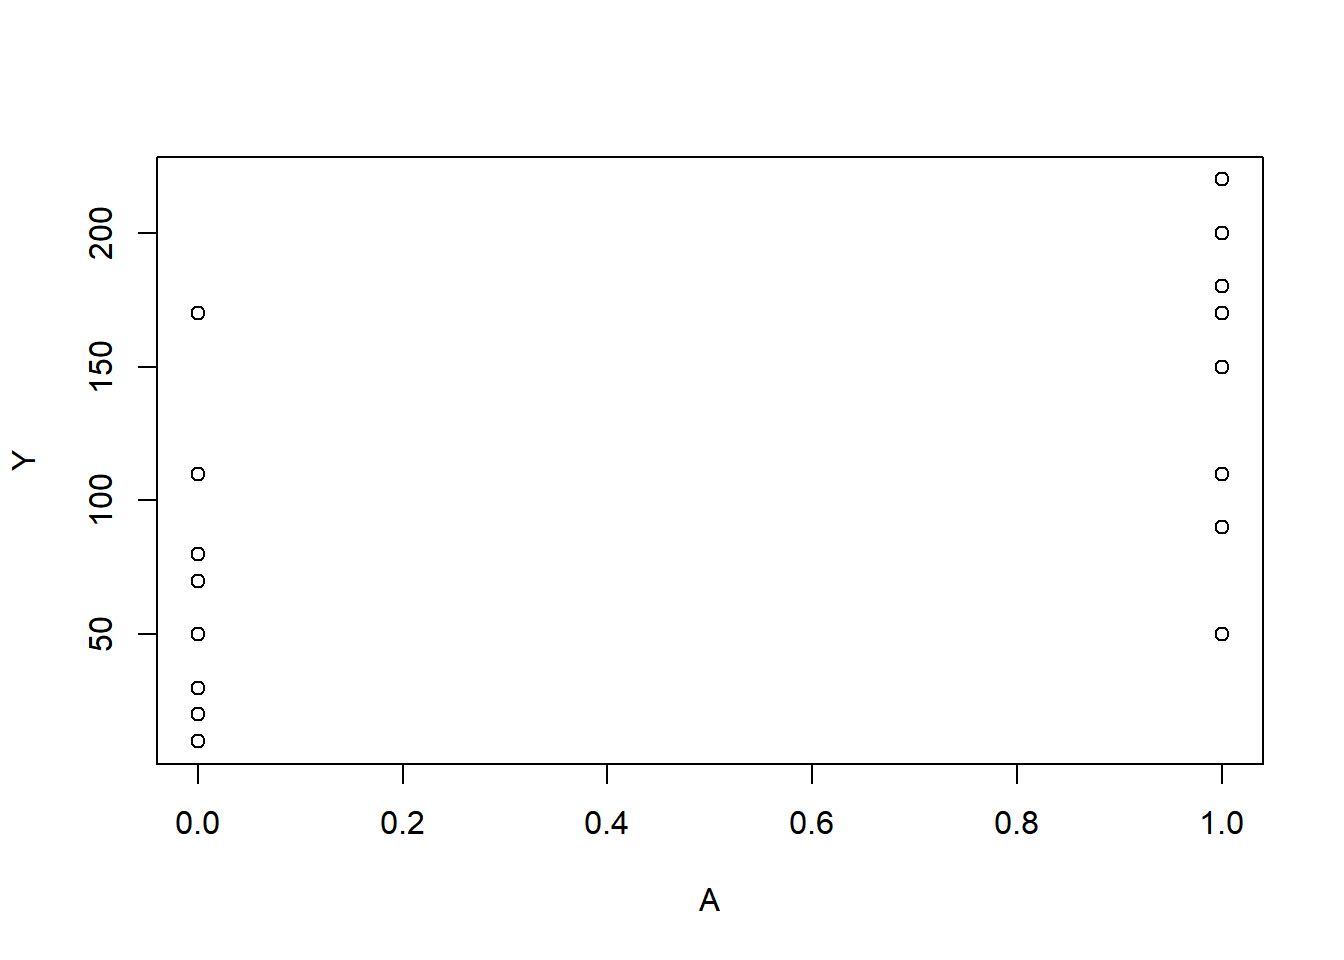
\includegraphics[width=0.85\linewidth]{17-causal-surv-r_files/figure-latex/unnamed-chunk-4-1} \end{center}

\hypertarget{program-17.4}{%
\section{Program 17.4}\label{program-17.4}}

\begin{itemize}
\tightlist
\item
  Estimating of survival curves via g-formula
\item
  Data from NHEFS
\end{itemize}

\begin{Shaded}
\begin{Highlighting}[]
\CommentTok{# fit of hazards model with covariates}
\NormalTok{gf.model <-}\StringTok{ }\KeywordTok{glm}\NormalTok{(event}\OperatorTok{==}\DecValTok{0} \OperatorTok{~}\StringTok{ }\NormalTok{qsmk }\OperatorTok{+}\StringTok{ }\KeywordTok{I}\NormalTok{(qsmk}\OperatorTok{*}\NormalTok{time) }\OperatorTok{+}\StringTok{ }\KeywordTok{I}\NormalTok{(qsmk}\OperatorTok{*}\NormalTok{timesq)}
                \OperatorTok{+}\StringTok{ }\NormalTok{time }\OperatorTok{+}\StringTok{ }\NormalTok{timesq }\OperatorTok{+}\StringTok{ }\NormalTok{sex }\OperatorTok{+}\StringTok{ }\NormalTok{race }\OperatorTok{+}\StringTok{ }\NormalTok{age }\OperatorTok{+}\StringTok{ }\KeywordTok{I}\NormalTok{(age}\OperatorTok{*}\NormalTok{age)}
                \OperatorTok{+}\StringTok{ }\KeywordTok{as.factor}\NormalTok{(education) }\OperatorTok{+}\StringTok{ }\NormalTok{smokeintensity }
                \OperatorTok{+}\StringTok{ }\KeywordTok{I}\NormalTok{(smokeintensity}\OperatorTok{*}\NormalTok{smokeintensity) }\OperatorTok{+}\StringTok{ }\NormalTok{smkintensity82_}\DecValTok{71} 
                \OperatorTok{+}\StringTok{ }\NormalTok{smokeyrs }\OperatorTok{+}\StringTok{ }\KeywordTok{I}\NormalTok{(smokeyrs}\OperatorTok{*}\NormalTok{smokeyrs) }\OperatorTok{+}\StringTok{ }\KeywordTok{as.factor}\NormalTok{(exercise) }
                \OperatorTok{+}\StringTok{ }\KeywordTok{as.factor}\NormalTok{(active) }\OperatorTok{+}\StringTok{ }\NormalTok{wt71 }\OperatorTok{+}\StringTok{ }\KeywordTok{I}\NormalTok{(wt71}\OperatorTok{*}\NormalTok{wt71), }
                \DataTypeTok{data=}\NormalTok{nhefs.surv, }\DataTypeTok{family=}\KeywordTok{binomial}\NormalTok{())}
\KeywordTok{summary}\NormalTok{(gf.model)}
\end{Highlighting}
\end{Shaded}

\begin{verbatim}
## 
## Call:
## glm(formula = event == 0 ~ qsmk + I(qsmk * time) + I(qsmk * timesq) + 
##     time + timesq + sex + race + age + I(age * age) + as.factor(education) + 
##     smokeintensity + I(smokeintensity * smokeintensity) + smkintensity82_71 + 
##     smokeyrs + I(smokeyrs * smokeyrs) + as.factor(exercise) + 
##     as.factor(active) + wt71 + I(wt71 * wt71), family = binomial(), 
##     data = nhefs.surv)
## 
## Deviance Residuals: 
##     Min       1Q   Median       3Q      Max  
## -4.3160   0.0244   0.0395   0.0640   0.3303  
## 
## Coefficients:
##                                      Estimate Std. Error z value Pr(>|z|)
## (Intercept)                         9.272e+00  1.379e+00   6.724 1.76e-11
## qsmk                                5.959e-02  4.154e-01   0.143 0.885924
## I(qsmk * time)                     -1.485e-02  1.506e-02  -0.987 0.323824
## I(qsmk * timesq)                    1.702e-04  1.245e-04   1.367 0.171643
## time                               -2.270e-02  8.437e-03  -2.690 0.007142
## timesq                              1.174e-04  6.709e-05   1.751 0.080020
## sex                                 4.368e-01  1.409e-01   3.101 0.001930
## race                               -5.240e-02  1.734e-01  -0.302 0.762572
## age                                -8.750e-02  5.907e-02  -1.481 0.138536
## I(age * age)                        8.128e-05  5.470e-04   0.149 0.881865
## as.factor(education)2               1.401e-01  1.566e-01   0.895 0.370980
## as.factor(education)3               4.335e-01  1.526e-01   2.841 0.004502
## as.factor(education)4               2.350e-01  2.790e-01   0.842 0.399750
## as.factor(education)5               3.750e-01  2.386e-01   1.571 0.116115
## smokeintensity                     -1.626e-03  1.430e-02  -0.114 0.909431
## I(smokeintensity * smokeintensity) -7.182e-05  2.390e-04  -0.301 0.763741
## smkintensity82_71                  -1.686e-03  6.501e-03  -0.259 0.795399
## smokeyrs                           -1.677e-02  3.065e-02  -0.547 0.584153
## I(smokeyrs * smokeyrs)             -5.280e-05  4.244e-04  -0.124 0.900997
## as.factor(exercise)1                1.469e-01  1.792e-01   0.820 0.412300
## as.factor(exercise)2               -1.504e-01  1.762e-01  -0.854 0.393177
## as.factor(active)1                 -1.601e-01  1.300e-01  -1.232 0.218048
## as.factor(active)2                 -2.294e-01  1.877e-01  -1.222 0.221766
## wt71                                6.222e-02  1.902e-02   3.271 0.001073
## I(wt71 * wt71)                     -4.046e-04  1.129e-04  -3.584 0.000338
##                                       
## (Intercept)                        ***
## qsmk                                  
## I(qsmk * time)                        
## I(qsmk * timesq)                      
## time                               ** 
## timesq                             .  
## sex                                ** 
## race                                  
## age                                   
## I(age * age)                          
## as.factor(education)2                 
## as.factor(education)3              ** 
## as.factor(education)4                 
## as.factor(education)5                 
## smokeintensity                        
## I(smokeintensity * smokeintensity)    
## smkintensity82_71                     
## smokeyrs                              
## I(smokeyrs * smokeyrs)                
## as.factor(exercise)1                  
## as.factor(exercise)2                  
## as.factor(active)1                    
## as.factor(active)2                    
## wt71                               ** 
## I(wt71 * wt71)                     ***
## ---
## Signif. codes:  0 '***' 0.001 '**' 0.01 '*' 0.05 '.' 0.1 ' ' 1
## 
## (Dispersion parameter for binomial family taken to be 1)
## 
##     Null deviance: 4655.3  on 176763  degrees of freedom
## Residual deviance: 4185.7  on 176739  degrees of freedom
## AIC: 4235.7
## 
## Number of Fisher Scoring iterations: 10
\end{verbatim}

\begin{Shaded}
\begin{Highlighting}[]
\CommentTok{# creation of dataset with all time points for }
\CommentTok{# each individual under each treatment level}
\NormalTok{gf.qsmk0 <-}\StringTok{ }\KeywordTok{expandRows}\NormalTok{(nhefs, }\DataTypeTok{count=}\DecValTok{120}\NormalTok{, }\DataTypeTok{count.is.col=}\NormalTok{F) }
\NormalTok{gf.qsmk0}\OperatorTok{$}\NormalTok{time <-}\StringTok{ }\KeywordTok{rep}\NormalTok{(}\KeywordTok{seq}\NormalTok{(}\DecValTok{0}\NormalTok{, }\DecValTok{119}\NormalTok{), }\KeywordTok{nrow}\NormalTok{(nhefs))}
\NormalTok{gf.qsmk0}\OperatorTok{$}\NormalTok{timesq <-}\StringTok{ }\NormalTok{gf.qsmk0}\OperatorTok{$}\NormalTok{time}\OperatorTok{^}\DecValTok{2}
\NormalTok{gf.qsmk0}\OperatorTok{$}\NormalTok{qsmk <-}\StringTok{ }\DecValTok{0}

\NormalTok{gf.qsmk1 <-}\StringTok{ }\NormalTok{gf.qsmk0}
\NormalTok{gf.qsmk1}\OperatorTok{$}\NormalTok{qsmk <-}\StringTok{ }\DecValTok{1}

\NormalTok{gf.qsmk0}\OperatorTok{$}\NormalTok{p.noevent0 <-}\StringTok{ }\KeywordTok{predict}\NormalTok{(gf.model, gf.qsmk0, }\DataTypeTok{type=}\StringTok{"response"}\NormalTok{)}
\NormalTok{gf.qsmk1}\OperatorTok{$}\NormalTok{p.noevent1 <-}\StringTok{ }\KeywordTok{predict}\NormalTok{(gf.model, gf.qsmk1, }\DataTypeTok{type=}\StringTok{"response"}\NormalTok{)}

\CommentTok{#install.packages("dplyr")}
\KeywordTok{library}\NormalTok{(}\StringTok{"dplyr"}\NormalTok{)}
\end{Highlighting}
\end{Shaded}

\begin{verbatim}
## 
## Attaching package: 'dplyr'
\end{verbatim}

\begin{verbatim}
## The following objects are masked from 'package:stats':
## 
##     filter, lag
\end{verbatim}

\begin{verbatim}
## The following objects are masked from 'package:base':
## 
##     intersect, setdiff, setequal, union
\end{verbatim}

\begin{Shaded}
\begin{Highlighting}[]
\NormalTok{gf.qsmk0.surv <-}\StringTok{ }\NormalTok{gf.qsmk0 }\OperatorTok\StringTok{ }\KeywordTok{group_by}\NormalTok{(seqn) }\OperatorTok\StringTok{ }\KeywordTok{mutate}\NormalTok{(}\DataTypeTok{surv0 =} \KeywordTok{cumprod}\NormalTok{(p.noevent0))}
\NormalTok{gf.qsmk1.surv <-}\StringTok{ }\NormalTok{gf.qsmk1 }\OperatorTok\StringTok{ }\KeywordTok{group_by}\NormalTok{(seqn) }\OperatorTok\StringTok{ }\KeywordTok{mutate}\NormalTok{(}\DataTypeTok{surv1 =} \KeywordTok{cumprod}\NormalTok{(p.noevent1))}

\NormalTok{gf.surv0 <-}\StringTok{ }\KeywordTok{aggregate}\NormalTok{(gf.qsmk0.surv, }\DataTypeTok{by=}\KeywordTok{list}\NormalTok{(gf.qsmk0.surv}\OperatorTok{$}\NormalTok{time), }\DataTypeTok{FUN=}\NormalTok{mean)[}\KeywordTok{c}\NormalTok{(}\StringTok{"qsmk"}\NormalTok{, }\StringTok{"time"}\NormalTok{, }\StringTok{"surv0"}\NormalTok{)]}
\NormalTok{gf.surv1 <-}\StringTok{ }\KeywordTok{aggregate}\NormalTok{(gf.qsmk1.surv, }\DataTypeTok{by=}\KeywordTok{list}\NormalTok{(gf.qsmk1.surv}\OperatorTok{$}\NormalTok{time), }\DataTypeTok{FUN=}\NormalTok{mean)[}\KeywordTok{c}\NormalTok{(}\StringTok{"qsmk"}\NormalTok{, }\StringTok{"time"}\NormalTok{, }\StringTok{"surv1"}\NormalTok{)]}

\NormalTok{gf.graph <-}\StringTok{ }\KeywordTok{merge}\NormalTok{(gf.surv0, gf.surv1, }\DataTypeTok{by=}\KeywordTok{c}\NormalTok{(}\StringTok{"time"}\NormalTok{))}
\NormalTok{gf.graph}\OperatorTok{$}\NormalTok{survdiff <-}\StringTok{ }\NormalTok{gf.graph}\OperatorTok{$}\NormalTok{surv1}\OperatorTok{-}\NormalTok{gf.graph}\OperatorTok{$}\NormalTok{surv0}

\CommentTok{# plot}
\KeywordTok{ggplot}\NormalTok{(gf.graph, }\KeywordTok{aes}\NormalTok{(}\DataTypeTok{x=}\NormalTok{time, }\DataTypeTok{y=}\NormalTok{surv)) }\OperatorTok{+}\StringTok{ }
\StringTok{  }\KeywordTok{geom_line}\NormalTok{(}\KeywordTok{aes}\NormalTok{(}\DataTypeTok{y =}\NormalTok{ surv0, }\DataTypeTok{colour =} \StringTok{"0"}\NormalTok{)) }\OperatorTok{+}\StringTok{ }
\StringTok{  }\KeywordTok{geom_line}\NormalTok{(}\KeywordTok{aes}\NormalTok{(}\DataTypeTok{y =}\NormalTok{ surv1, }\DataTypeTok{colour =} \StringTok{"1"}\NormalTok{)) }\OperatorTok{+}\StringTok{ }
\StringTok{  }\KeywordTok{xlab}\NormalTok{(}\StringTok{"Months"}\NormalTok{) }\OperatorTok{+}\StringTok{ }
\StringTok{  }\KeywordTok{scale_x_continuous}\NormalTok{(}\DataTypeTok{limits =} \KeywordTok{c}\NormalTok{(}\DecValTok{0}\NormalTok{, }\DecValTok{120}\NormalTok{), }\DataTypeTok{breaks=}\KeywordTok{seq}\NormalTok{(}\DecValTok{0}\NormalTok{,}\DecValTok{120}\NormalTok{,}\DecValTok{12}\NormalTok{)) }\OperatorTok{+}
\StringTok{  }\KeywordTok{scale_y_continuous}\NormalTok{(}\DataTypeTok{limits=}\KeywordTok{c}\NormalTok{(}\FloatTok{0.6}\NormalTok{, }\DecValTok{1}\NormalTok{), }\DataTypeTok{breaks=}\KeywordTok{seq}\NormalTok{(}\FloatTok{0.6}\NormalTok{, }\DecValTok{1}\NormalTok{, }\FloatTok{0.2}\NormalTok{)) }\OperatorTok{+}
\StringTok{  }\KeywordTok{ylab}\NormalTok{(}\StringTok{"Survival"}\NormalTok{) }\OperatorTok{+}\StringTok{ }
\StringTok{  }\KeywordTok{ggtitle}\NormalTok{(}\StringTok{"Survival from g-formula"}\NormalTok{) }\OperatorTok{+}\StringTok{ }
\StringTok{  }\KeywordTok{labs}\NormalTok{(}\DataTypeTok{colour=}\StringTok{"A:"}\NormalTok{) }\OperatorTok{+}
\StringTok{  }\KeywordTok{theme_bw}\NormalTok{() }\OperatorTok{+}\StringTok{ }
\StringTok{  }\KeywordTok{theme}\NormalTok{(}\DataTypeTok{legend.position=}\StringTok{"bottom"}\NormalTok{)}
\end{Highlighting}
\end{Shaded}

\begin{center}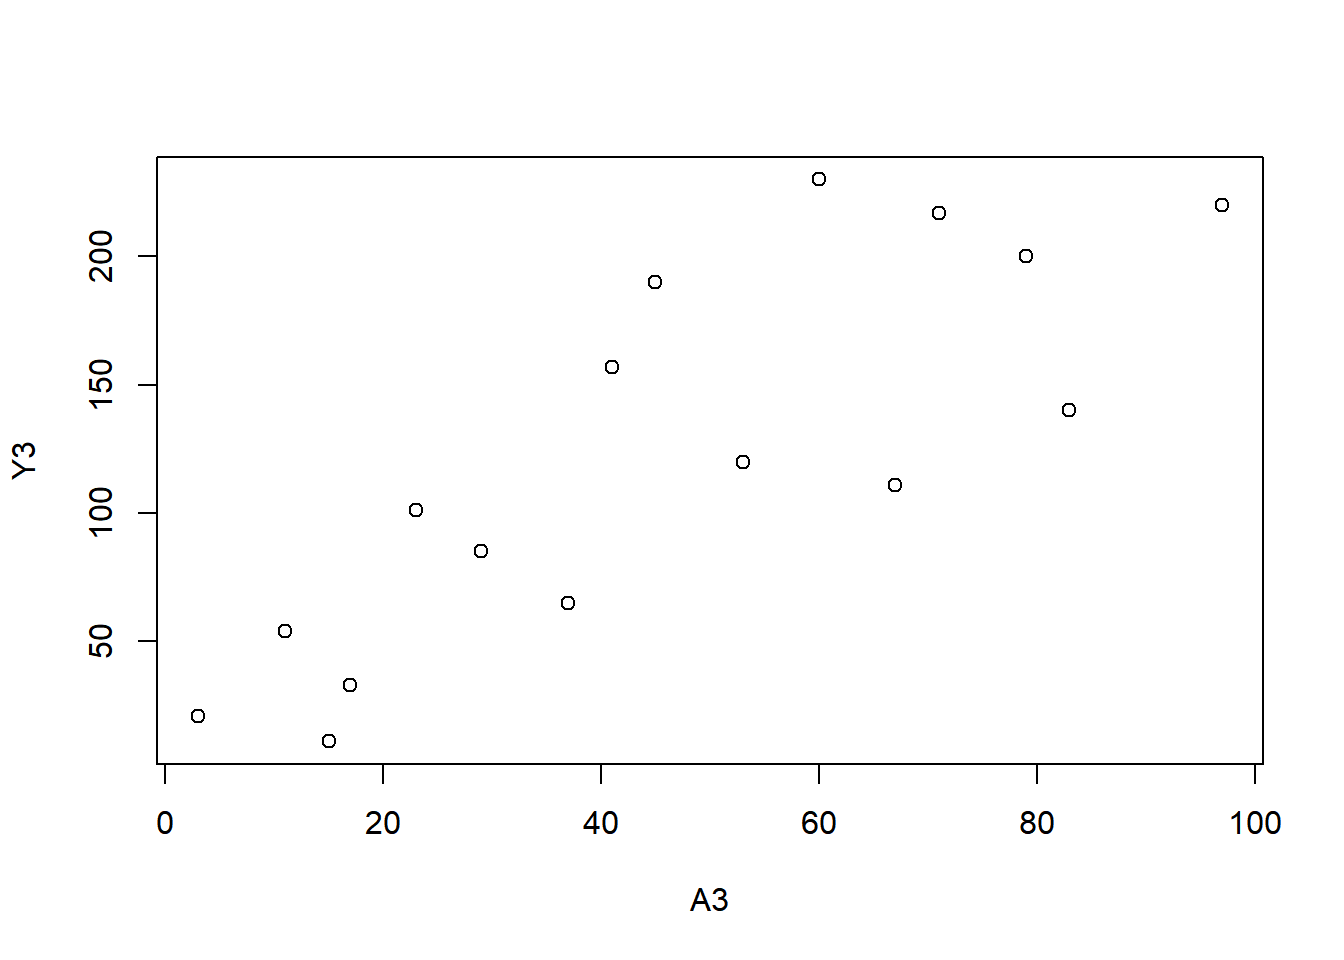
\includegraphics[width=0.85\linewidth]{17-causal-surv-r_files/figure-latex/unnamed-chunk-5-1} \end{center}

\hypertarget{program-17.5}{%
\section{Program 17.5}\label{program-17.5}}

\begin{itemize}
\tightlist
\item
  Estimating of median survival time ratio via a structural nested AFT model
\item
  Data from NHEFS
\end{itemize}

\begin{Shaded}
\begin{Highlighting}[]
\CommentTok{# some preprocessing of the data}
\NormalTok{nhefs <-}\StringTok{ }\KeywordTok{read_excel}\NormalTok{(}\KeywordTok{here}\NormalTok{(}\StringTok{"data"}\NormalTok{, }\StringTok{"NHEFS.xls"}\NormalTok{))}
\NormalTok{nhefs}\OperatorTok{$}\NormalTok{survtime <-}\StringTok{ }\KeywordTok{ifelse}\NormalTok{(nhefs}\OperatorTok{$}\NormalTok{death}\OperatorTok{==}\DecValTok{0}\NormalTok{, }\OtherTok{NA}\NormalTok{, (nhefs}\OperatorTok{$}\NormalTok{yrdth}\DecValTok{-83}\NormalTok{)}\OperatorTok{*}\DecValTok{12}\OperatorTok{+}\NormalTok{nhefs}\OperatorTok{$}\NormalTok{modth) }\CommentTok{# * yrdth ranges from 83 to 92}

\CommentTok{# model to estimate E[A|L]}
\NormalTok{modelA <-}\StringTok{ }\KeywordTok{glm}\NormalTok{(qsmk }\OperatorTok{~}\StringTok{ }\NormalTok{sex }\OperatorTok{+}\StringTok{ }\NormalTok{race }\OperatorTok{+}\StringTok{ }\NormalTok{age }\OperatorTok{+}\StringTok{ }\KeywordTok{I}\NormalTok{(age}\OperatorTok{*}\NormalTok{age)}
              \OperatorTok{+}\StringTok{ }\KeywordTok{as.factor}\NormalTok{(education) }\OperatorTok{+}\StringTok{ }\NormalTok{smokeintensity}
              \OperatorTok{+}\StringTok{ }\KeywordTok{I}\NormalTok{(smokeintensity}\OperatorTok{*}\NormalTok{smokeintensity) }\OperatorTok{+}\StringTok{ }\NormalTok{smokeyrs}
              \OperatorTok{+}\StringTok{ }\KeywordTok{I}\NormalTok{(smokeyrs}\OperatorTok{*}\NormalTok{smokeyrs) }\OperatorTok{+}\StringTok{ }\KeywordTok{as.factor}\NormalTok{(exercise)}
              \OperatorTok{+}\StringTok{ }\KeywordTok{as.factor}\NormalTok{(active) }\OperatorTok{+}\StringTok{ }\NormalTok{wt71 }\OperatorTok{+}\StringTok{ }\KeywordTok{I}\NormalTok{(wt71}\OperatorTok{*}\NormalTok{wt71),}
              \DataTypeTok{data=}\NormalTok{nhefs, }\DataTypeTok{family=}\KeywordTok{binomial}\NormalTok{())}

\NormalTok{nhefs}\OperatorTok{$}\NormalTok{p.qsmk <-}\StringTok{ }\KeywordTok{predict}\NormalTok{(modelA, nhefs, }\DataTypeTok{type=}\StringTok{"response"}\NormalTok{) }
\NormalTok{d <-}\StringTok{ }\NormalTok{nhefs[}\OperatorTok{!}\KeywordTok{is.na}\NormalTok{(nhefs}\OperatorTok{$}\NormalTok{survtime),] }\CommentTok{# select only those with observed death time}
\NormalTok{n <-}\StringTok{ }\KeywordTok{nrow}\NormalTok{(d)}

\CommentTok{# define the estimating function that needs to be minimized}
\NormalTok{sumeef <-}\StringTok{ }\ControlFlowTok{function}\NormalTok{(psi)\{}
  
  \CommentTok{# creation of delta indicator}
  \ControlFlowTok{if}\NormalTok{ (psi}\OperatorTok{>=}\DecValTok{0}\NormalTok{)\{}
\NormalTok{    delta <-}\StringTok{ }\KeywordTok{ifelse}\NormalTok{(d}\OperatorTok{$}\NormalTok{qsmk}\OperatorTok{==}\DecValTok{0} \OperatorTok{|}\StringTok{ }
\StringTok{                      }\NormalTok{(d}\OperatorTok{$}\NormalTok{qsmk}\OperatorTok{==}\DecValTok{1} \OperatorTok{&}\StringTok{ }\NormalTok{psi }\OperatorTok{<=}\StringTok{ }\KeywordTok{log}\NormalTok{(}\DecValTok{120}\OperatorTok{/}\NormalTok{d}\OperatorTok{$}\NormalTok{survtime)), }
                    \DecValTok{1}\NormalTok{, }\DecValTok{0}\NormalTok{)}
\NormalTok{  \} }\ControlFlowTok{else} \ControlFlowTok{if}\NormalTok{ (psi }\OperatorTok{<}\StringTok{ }\DecValTok{0}\NormalTok{) \{}
\NormalTok{    delta <-}\StringTok{ }\KeywordTok{ifelse}\NormalTok{(d}\OperatorTok{$}\NormalTok{qsmk}\OperatorTok{==}\DecValTok{1} \OperatorTok{|}\StringTok{ }
\StringTok{                      }\NormalTok{(d}\OperatorTok{$}\NormalTok{qsmk}\OperatorTok{==}\DecValTok{0} \OperatorTok{&}\StringTok{ }\NormalTok{psi }\OperatorTok{>}\StringTok{ }\KeywordTok{log}\NormalTok{(d}\OperatorTok{$}\NormalTok{survtime}\OperatorTok{/}\DecValTok{120}\NormalTok{)), }\DecValTok{1}\NormalTok{, }\DecValTok{0}\NormalTok{)}
\NormalTok{  \}}
  
\NormalTok{  smat <-}\StringTok{ }\NormalTok{delta}\OperatorTok{*}\NormalTok{(d}\OperatorTok{$}\NormalTok{qsmk}\OperatorTok{-}\NormalTok{d}\OperatorTok{$}\NormalTok{p.qsmk)}
\NormalTok{  sval <-}\StringTok{ }\KeywordTok{sum}\NormalTok{(smat, }\DataTypeTok{na.rm=}\NormalTok{T)}
\NormalTok{  save <-}\StringTok{ }\NormalTok{sval}\OperatorTok{/}\NormalTok{n}
\NormalTok{  smat <-}\StringTok{ }\NormalTok{smat }\OperatorTok{-}\StringTok{ }\KeywordTok{rep}\NormalTok{(save, n)}
  
  \CommentTok{# covariance}
\NormalTok{  sigma <-}\StringTok{ }\KeywordTok{t}\NormalTok{(smat) }\OperatorTok\StringTok{ }\NormalTok{smat}
  \ControlFlowTok{if}\NormalTok{ (sigma }\OperatorTok{==}\StringTok{ }\DecValTok{0}\NormalTok{)\{}
\NormalTok{    sigma <-}\StringTok{ }\FloatTok{1e-16}
\NormalTok{  \}}
\NormalTok{  estimeq <-}\StringTok{ }\NormalTok{sval}\OperatorTok{*}\KeywordTok{solve}\NormalTok{(sigma)}\OperatorTok{*}\KeywordTok{t}\NormalTok{(sval)}
  \KeywordTok{return}\NormalTok{(estimeq)}
\NormalTok{\}}

\NormalTok{res <-}\StringTok{ }\KeywordTok{optimize}\NormalTok{(sumeef, }\DataTypeTok{interval =} \KeywordTok{c}\NormalTok{(}\OperatorTok{-}\FloatTok{0.2}\NormalTok{,}\FloatTok{0.2}\NormalTok{))}
\NormalTok{psi1 <-}\StringTok{ }\NormalTok{res}\OperatorTok{$}\NormalTok{minimum}
\NormalTok{objfunc <-}\StringTok{ }\KeywordTok{as.numeric}\NormalTok{(res}\OperatorTok{$}\NormalTok{objective)}


\CommentTok{# Use simple bisection method to find estimates of lower and upper 95% confidence bounds}
\NormalTok{increm <-}\StringTok{ }\FloatTok{0.1}
\NormalTok{for_conf <-}\StringTok{ }\ControlFlowTok{function}\NormalTok{(x)\{}
  \KeywordTok{return}\NormalTok{(}\KeywordTok{sumeef}\NormalTok{(x) }\OperatorTok{-}\StringTok{ }\FloatTok{3.84}\NormalTok{)}
\NormalTok{\}}

\ControlFlowTok{if}\NormalTok{ (objfunc }\OperatorTok{<}\StringTok{ }\FloatTok{3.84}\NormalTok{)\{}
  \CommentTok{# Find estimate of where sumeef(x) > 3.84}
  
  \CommentTok{# Lower bound of 95% CI}
\NormalTok{  psilow <-}\StringTok{ }\NormalTok{psi1}
\NormalTok{  testlow <-}\StringTok{ }\NormalTok{objfunc}
\NormalTok{  countlow <-}\StringTok{ }\DecValTok{0}
  \ControlFlowTok{while}\NormalTok{ (testlow }\OperatorTok{<}\StringTok{ }\FloatTok{3.84} \OperatorTok{&}\StringTok{ }\NormalTok{countlow }\OperatorTok{<}\StringTok{ }\DecValTok{100}\NormalTok{)\{}
\NormalTok{    psilow <-}\StringTok{ }\NormalTok{psilow }\OperatorTok{-}\StringTok{ }\NormalTok{increm}
\NormalTok{    testlow <-}\StringTok{ }\KeywordTok{sumeef}\NormalTok{(psilow)}
\NormalTok{    countlow <-}\StringTok{ }\NormalTok{countlow }\OperatorTok{+}\StringTok{ }\DecValTok{1}
\NormalTok{  \}}
  
  \CommentTok{# Upper bound of 95% CI}
\NormalTok{  psihigh <-}\StringTok{ }\NormalTok{psi1}
\NormalTok{  testhigh <-}\StringTok{ }\NormalTok{objfunc}
\NormalTok{  counthigh <-}\StringTok{ }\DecValTok{0}
  \ControlFlowTok{while}\NormalTok{ (testhigh }\OperatorTok{<}\StringTok{ }\FloatTok{3.84} \OperatorTok{&}\StringTok{ }\NormalTok{counthigh }\OperatorTok{<}\StringTok{ }\DecValTok{100}\NormalTok{)\{}
\NormalTok{    psihigh <-}\StringTok{ }\NormalTok{psihigh }\OperatorTok{+}\StringTok{ }\NormalTok{increm}
\NormalTok{    testhigh <-}\StringTok{ }\KeywordTok{sumeef}\NormalTok{(psihigh)}
\NormalTok{    counthigh <-}\StringTok{ }\NormalTok{counthigh }\OperatorTok{+}\StringTok{ }\DecValTok{1}
\NormalTok{  \}}
  
  \CommentTok{# Better estimate using bisection method}
  \ControlFlowTok{if}\NormalTok{ ((testhigh }\OperatorTok{>}\StringTok{ }\FloatTok{3.84}\NormalTok{) }\OperatorTok{&}\StringTok{ }\NormalTok{(testlow }\OperatorTok{>}\StringTok{ }\FloatTok{3.84}\NormalTok{))\{}
    
    \CommentTok{# Bisection method}
\NormalTok{    left <-}\StringTok{ }\NormalTok{psi1}
\NormalTok{    fleft <-}\StringTok{ }\NormalTok{objfunc }\OperatorTok{-}\StringTok{ }\FloatTok{3.84}
\NormalTok{    right <-}\StringTok{ }\NormalTok{psihigh}
\NormalTok{    fright <-}\StringTok{ }\NormalTok{testhigh }\OperatorTok{-}\StringTok{ }\FloatTok{3.84}
\NormalTok{    middle <-}\StringTok{ }\NormalTok{(left  }\OperatorTok{+}\StringTok{ }\NormalTok{right) }\OperatorTok{/}\StringTok{ }\DecValTok{2}
\NormalTok{    fmiddle <-}\StringTok{ }\KeywordTok{for_conf}\NormalTok{(middle)}
\NormalTok{    count <-}\StringTok{ }\DecValTok{0}
\NormalTok{    diff <-}\StringTok{ }\NormalTok{right }\OperatorTok{-}\StringTok{ }\NormalTok{left}
    
    \ControlFlowTok{while}\NormalTok{ (}\OperatorTok{!}\NormalTok{(}\KeywordTok{abs}\NormalTok{(fmiddle) }\OperatorTok{<}\StringTok{ }\FloatTok{0.0001} \OperatorTok{|}\StringTok{ }\NormalTok{diff }\OperatorTok{<}\StringTok{ }\FloatTok{0.0001} \OperatorTok{|}\StringTok{ }\NormalTok{count }\OperatorTok{>}\StringTok{ }\DecValTok{100}\NormalTok{))\{}
\NormalTok{      test <-}\StringTok{ }\NormalTok{fmiddle }\OperatorTok{*}\StringTok{ }\NormalTok{fleft}
      \ControlFlowTok{if}\NormalTok{ (test }\OperatorTok{<}\StringTok{ }\DecValTok{0}\NormalTok{)\{}
\NormalTok{        right <-}\StringTok{ }\NormalTok{middle}
\NormalTok{        fright <-}\StringTok{ }\NormalTok{fmiddle}
\NormalTok{      \} }\ControlFlowTok{else}\NormalTok{ \{}
\NormalTok{        left <-}\StringTok{ }\NormalTok{middle}
\NormalTok{        fleft <-}\StringTok{ }\NormalTok{fmiddle}
\NormalTok{      \}}
\NormalTok{      middle <-}\StringTok{ }\NormalTok{(left }\OperatorTok{+}\StringTok{ }\NormalTok{right) }\OperatorTok{/}\StringTok{ }\DecValTok{2}
\NormalTok{      fmiddle <-}\StringTok{ }\KeywordTok{for_conf}\NormalTok{(middle)}
\NormalTok{      count <-}\StringTok{ }\NormalTok{count }\OperatorTok{+}\StringTok{ }\DecValTok{1}
\NormalTok{      diff <-}\StringTok{ }\NormalTok{right }\OperatorTok{-}\StringTok{ }\NormalTok{left}
\NormalTok{    \}}
    
\NormalTok{    psi_high <-}\StringTok{ }\NormalTok{middle}
\NormalTok{    objfunc_high <-}\StringTok{ }\NormalTok{fmiddle }\OperatorTok{+}\StringTok{ }\FloatTok{3.84}
    
    \CommentTok{# lower bound of 95% CI}
\NormalTok{    left <-}\StringTok{ }\NormalTok{psilow}
\NormalTok{    fleft <-}\StringTok{ }\NormalTok{testlow }\OperatorTok{-}\StringTok{ }\FloatTok{3.84}
\NormalTok{    right <-}\StringTok{ }\NormalTok{psi1}
\NormalTok{    fright <-}\StringTok{ }\NormalTok{objfunc }\OperatorTok{-}\StringTok{ }\FloatTok{3.84}
\NormalTok{    middle <-}\StringTok{ }\NormalTok{(left }\OperatorTok{+}\StringTok{ }\NormalTok{right) }\OperatorTok{/}\StringTok{ }\DecValTok{2}
\NormalTok{    fmiddle <-}\StringTok{ }\KeywordTok{for_conf}\NormalTok{(middle)}
\NormalTok{    count <-}\StringTok{ }\DecValTok{0}
\NormalTok{    diff <-}\StringTok{ }\NormalTok{right }\OperatorTok{-}\StringTok{ }\NormalTok{left}
    
    \ControlFlowTok{while}\NormalTok{(}\OperatorTok{!}\NormalTok{(}\KeywordTok{abs}\NormalTok{(fmiddle) }\OperatorTok{<}\StringTok{ }\FloatTok{0.0001} \OperatorTok{|}\StringTok{ }\NormalTok{diff }\OperatorTok{<}\StringTok{ }\FloatTok{0.0001} \OperatorTok{|}\StringTok{ }\NormalTok{count }\OperatorTok{>}\StringTok{ }\DecValTok{100}\NormalTok{))\{}
\NormalTok{      test <-}\StringTok{ }\NormalTok{fmiddle }\OperatorTok{*}\StringTok{ }\NormalTok{fleft}
      \ControlFlowTok{if}\NormalTok{ (test }\OperatorTok{<}\StringTok{ }\DecValTok{0}\NormalTok{)\{}
\NormalTok{        right <-}\StringTok{ }\NormalTok{middle}
\NormalTok{        fright <-}\StringTok{ }\NormalTok{fmiddle}
\NormalTok{      \} }\ControlFlowTok{else}\NormalTok{ \{}
\NormalTok{        left <-}\StringTok{ }\NormalTok{middle}
\NormalTok{        fleft <-}\StringTok{ }\NormalTok{fmiddle}
\NormalTok{      \}}
\NormalTok{      middle <-}\StringTok{ }\NormalTok{(left }\OperatorTok{+}\StringTok{ }\NormalTok{right) }\OperatorTok{/}\StringTok{ }\DecValTok{2}
\NormalTok{      fmiddle <-}\StringTok{ }\KeywordTok{for_conf}\NormalTok{(middle)}
\NormalTok{      diff <-}\StringTok{ }\NormalTok{right }\OperatorTok{-}\StringTok{ }\NormalTok{left}
\NormalTok{      count <-}\StringTok{ }\NormalTok{count }\OperatorTok{+}\StringTok{ }\DecValTok{1}
\NormalTok{    \}}
\NormalTok{    psi_low <-}\StringTok{ }\NormalTok{middle}
\NormalTok{    objfunc_low <-}\StringTok{ }\NormalTok{fmiddle }\OperatorTok{+}\StringTok{ }\FloatTok{3.84}
\NormalTok{    psi <-}\StringTok{ }\NormalTok{psi1}
\NormalTok{  \}}
\NormalTok{\}}
\KeywordTok{c}\NormalTok{(psi, psi_low, psi_high)}
\end{Highlighting}
\end{Shaded}

\begin{verbatim}
## [1] -0.05041591 -0.22312099  0.33312901
\end{verbatim}

\hypertarget{r-session-information}{%
\chapter*{R session information}\label{r-session-information}}
\addcontentsline{toc}{chapter}{R session information}

For reproducibility.

\begin{Shaded}
\begin{Highlighting}[]
\CommentTok{# install.packages("sessioninfo")}
\NormalTok{sessioninfo}\OperatorTok{::}\KeywordTok{session_info}\NormalTok{()}
\end{Highlighting}
\end{Shaded}

\begin{verbatim}
## - Session info ----------------------------------------------------------
##  setting  value                       
##  version  R version 3.6.1 (2019-07-05)
##  os       Windows 10 x64              
##  system   x86_64, mingw32             
##  ui       RTerm                       
##  language (EN)                        
##  collate  English_United Kingdom.1252 
##  ctype    English_United Kingdom.1252 
##  tz       Europe/London               
##  date     2019-10-01                  
## 
## - Packages --------------------------------------------------------------
##  package     * version date       lib source        
##  assertthat    0.2.1   2019-03-21 [1] CRAN (R 3.6.0)
##  bookdown      0.13    2019-08-21 [1] CRAN (R 3.6.1)
##  cli           1.1.0   2019-03-19 [1] CRAN (R 3.6.0)
##  crayon        1.3.4   2017-09-16 [1] CRAN (R 3.6.0)
##  digest        0.6.21  2019-09-20 [1] CRAN (R 3.6.1)
##  evaluate      0.14    2019-05-28 [1] CRAN (R 3.6.0)
##  htmltools     0.3.6   2017-04-28 [1] CRAN (R 3.6.0)
##  knitr         1.25    2019-09-18 [1] CRAN (R 3.6.1)
##  magrittr      1.5     2014-11-22 [1] CRAN (R 3.6.0)
##  Rcpp          1.0.2   2019-07-25 [1] CRAN (R 3.6.1)
##  rmarkdown     1.15    2019-08-21 [1] CRAN (R 3.6.1)
##  sessioninfo   1.1.1   2018-11-05 [1] CRAN (R 3.6.0)
##  stringi       1.4.3   2019-03-12 [1] CRAN (R 3.6.0)
##  stringr       1.4.0   2019-02-10 [1] CRAN (R 3.6.0)
##  withr         2.1.2   2018-03-15 [1] CRAN (R 3.6.0)
##  xfun          0.9     2019-08-21 [1] CRAN (R 3.6.1)
##  yaml          2.2.0   2018-07-25 [1] CRAN (R 3.6.0)
## 
## [1] C:/Users/palmertm/library
## [2] C:/Program Files/R/R-3.6.1/library
\end{verbatim}

\backmatter


\end{document}
